\thispagestyle{toancuabinone}
\pagestyle{toancuabi}
\everymath{\color{toancuabi}}
\blfootnote{$^1$\color{toancuabi}Trường Liên cấp Hội nhập Quốc tế iSchool Quảng Trị.}
\graphicspath{{../toancuabi/trochoi/}}
\begingroup
\AddToShipoutPicture*{\put(0,616){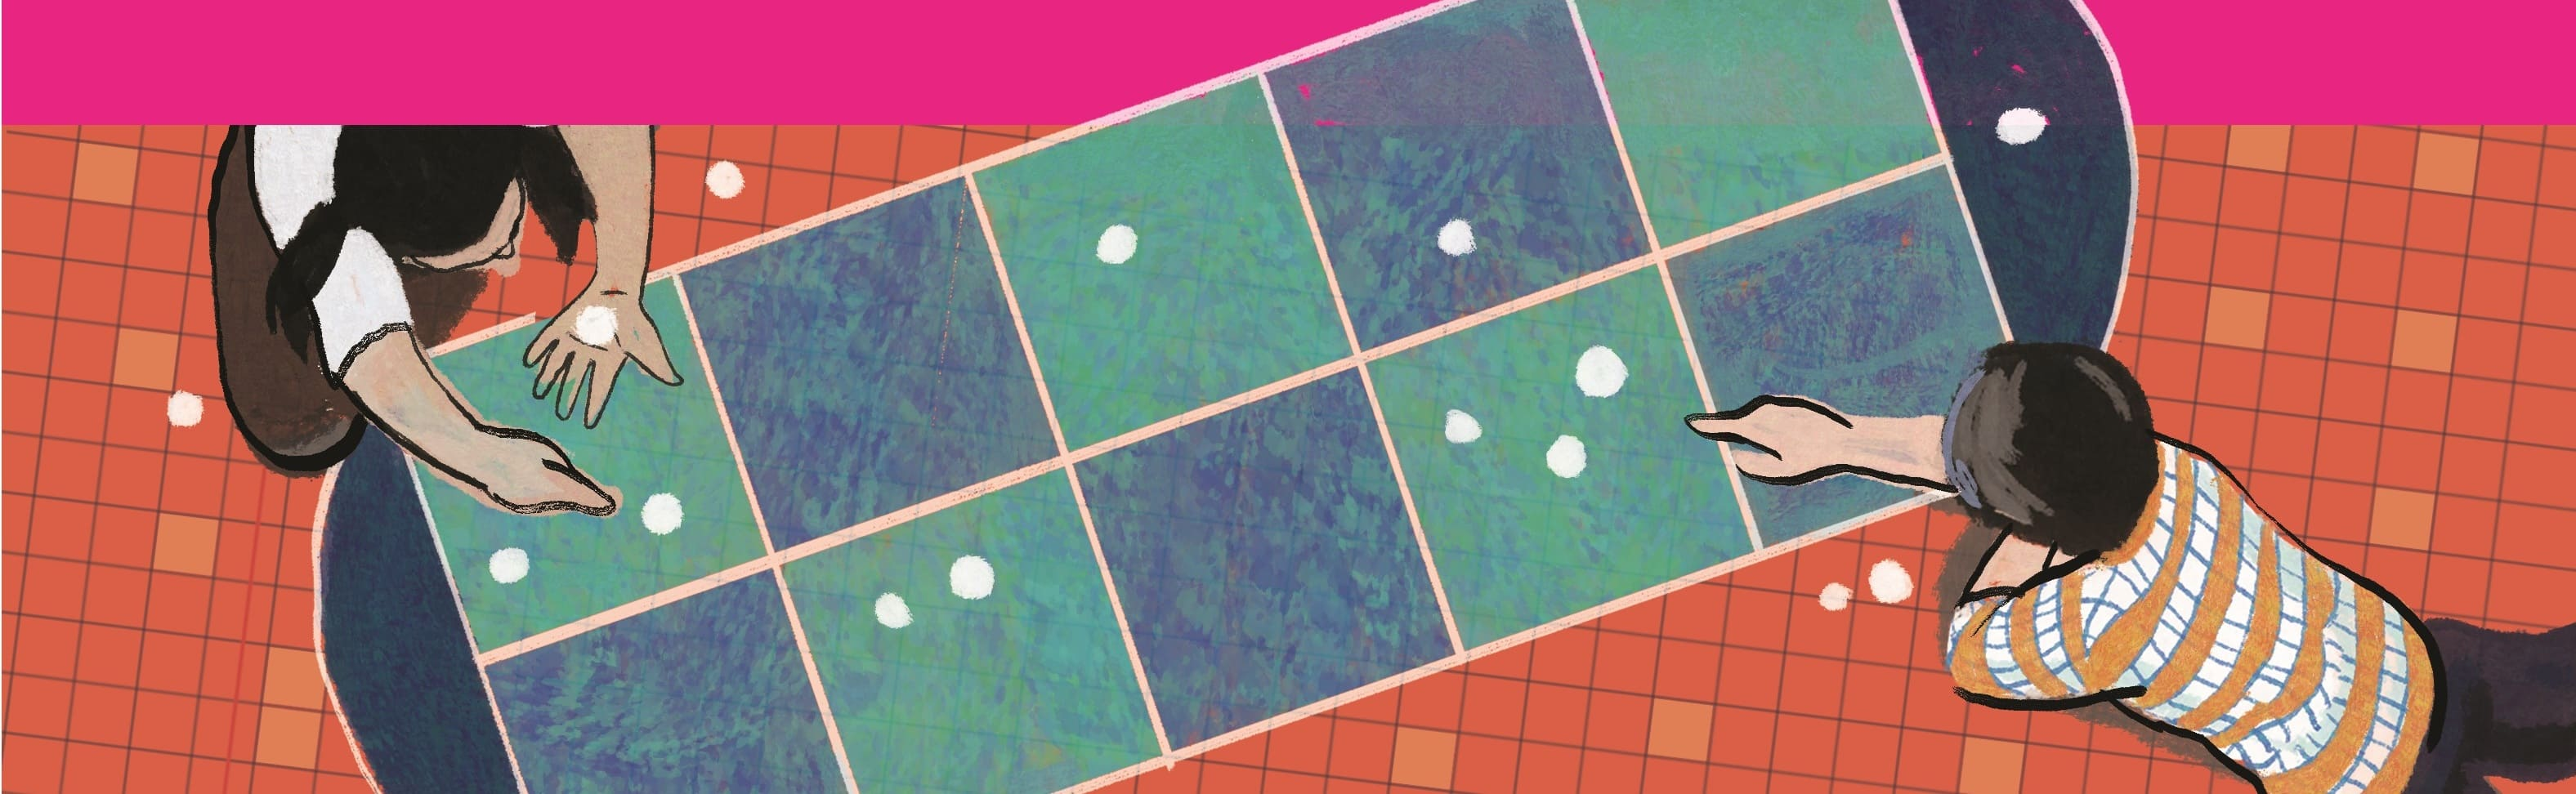
\includegraphics[width=19.3cm]{../bannertoancuabi}}}  
\AddToShipoutPicture*{\put(60,495){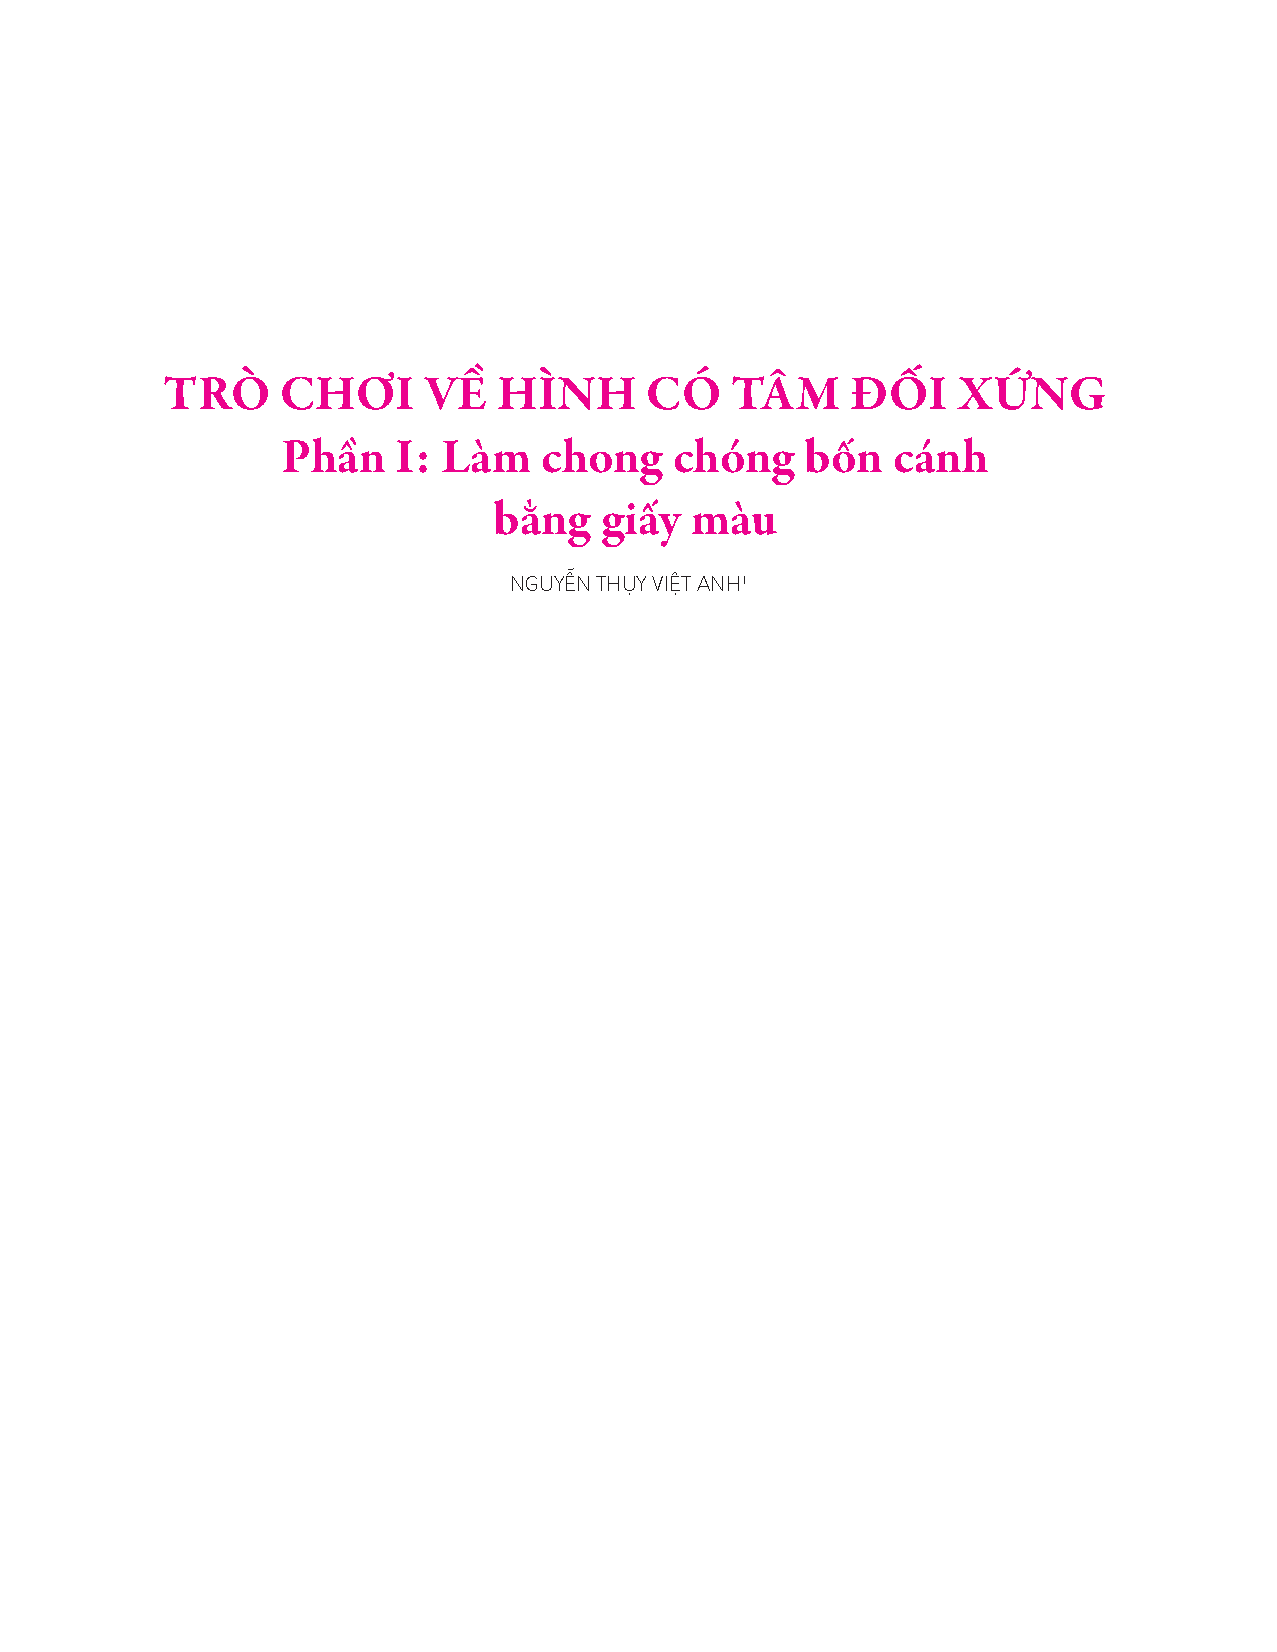
\includegraphics[scale=0.9]{../Untitled.pdf}}}  
\centering
\endgroup
\vspace*{207pt} 

\definecolor{bulgarianrose}{rgb}{0.28, 0.02, 0.03}
\begin{multicols}{2}
	Những chiếc chong chóng sặc sỡ sắc màu xoay trong gió sẽ làm dịu mát hơn những ngày hè nóng nực. Ngày hôm nay chúng ta sẽ cùng nhau làm nên những chiếc chong chóng tre từ giấy màu nhé!
	\vskip 0.1cm
	\textbf{\color{toancuabi}\textit{Chuẩn bị:}} Kéo, hồ dán, giấy màu, thước kẻ, bút chì, com--pa, kìm, dây thép.
	\vskip 0.1cm
	\textit{Bước $1$:} Cắt một tờ giấy màu hình vuông có độ dài mỗi cạnh là $14$cm.
	\begin{figure}[H]
		\vspace*{-5pt}
		\centering
		\captionsetup{labelformat= empty, justification=centering}
		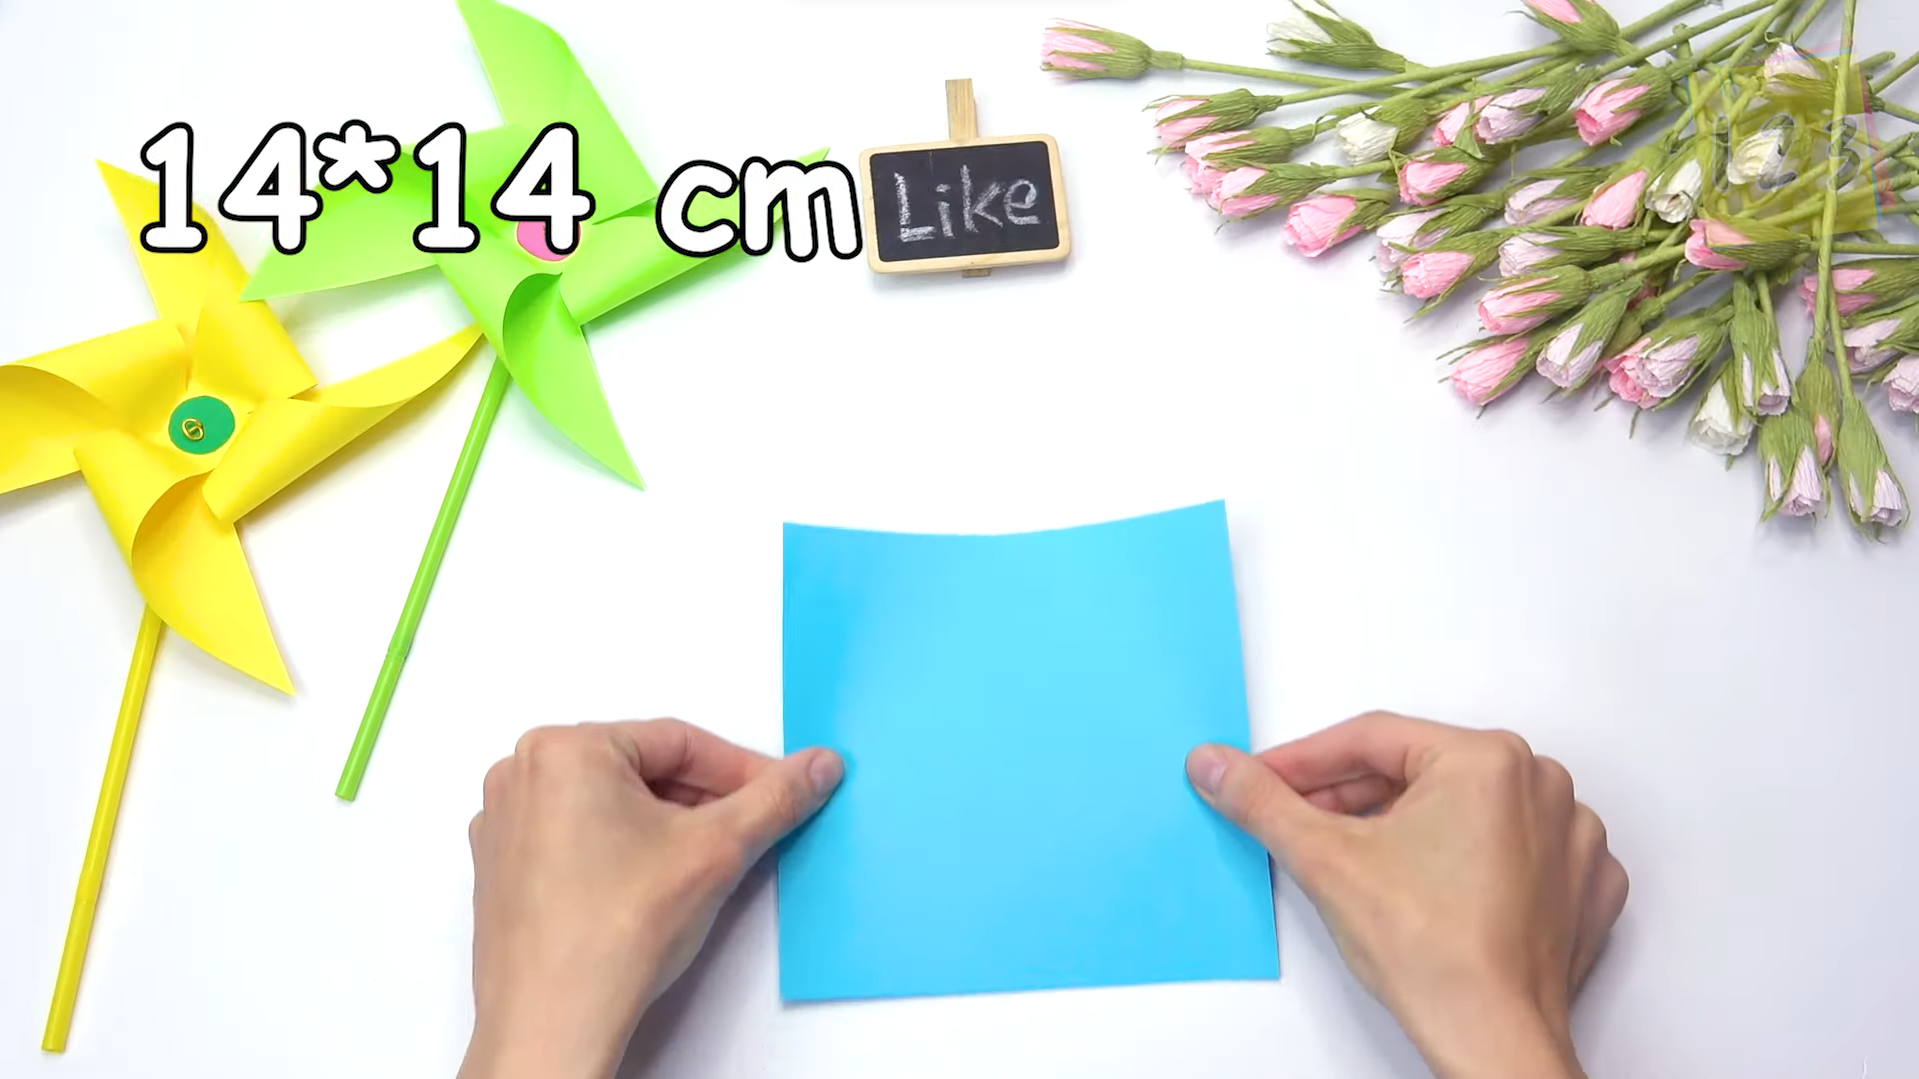
\includegraphics[width= 0.8\linewidth]{1}
		\vspace*{-10pt}
	\end{figure}
	\textit{Bước $2$:} Gấp đôi tờ giấy màu hình vuông theo các đường chéo để tạo nếp gấp, sau đó mở ra.
	\begin{figure}[H]
		\vspace*{-5pt}
		\centering
		\captionsetup{labelformat= empty, justification=centering}
		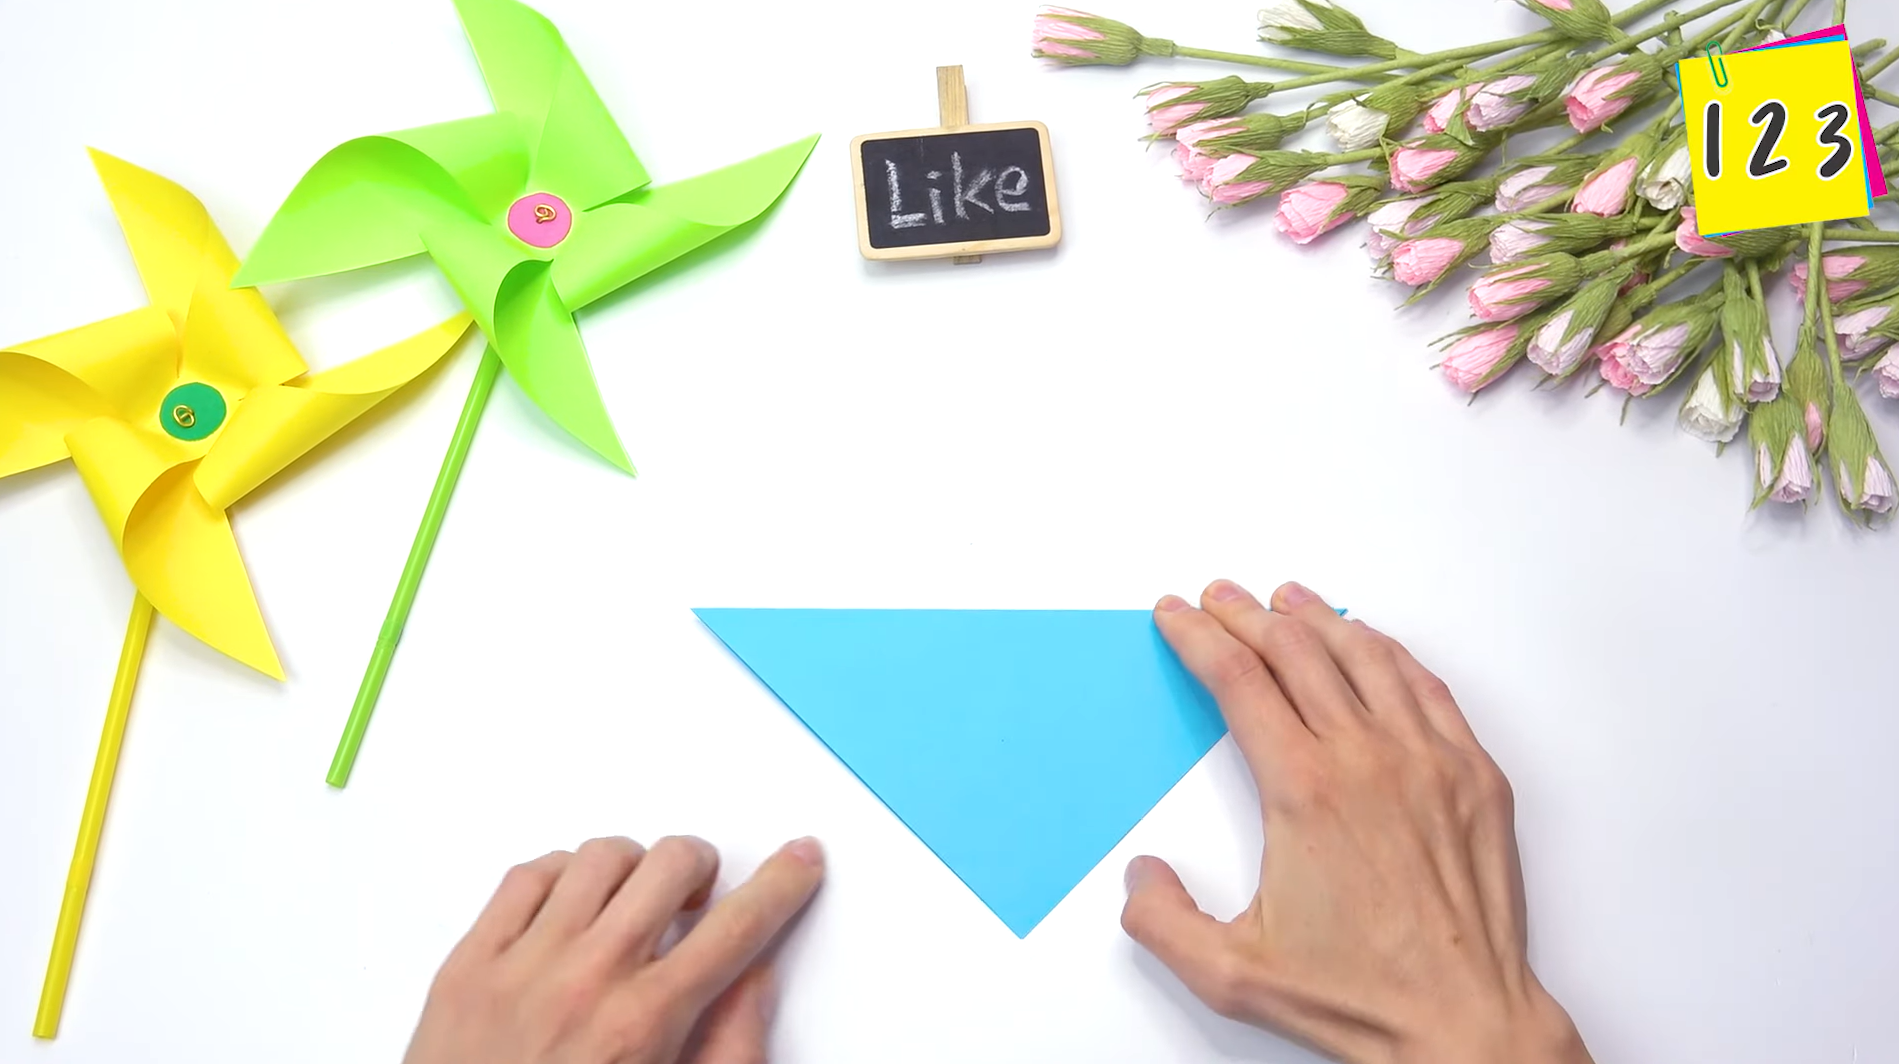
\includegraphics[width= 0.8\linewidth]{2a}
%		\vspace*{-5pt}
	\end{figure}
	\begin{figure}[H]
		\vspace*{5pt}
		\centering
		\captionsetup{labelformat= empty, justification=centering}
		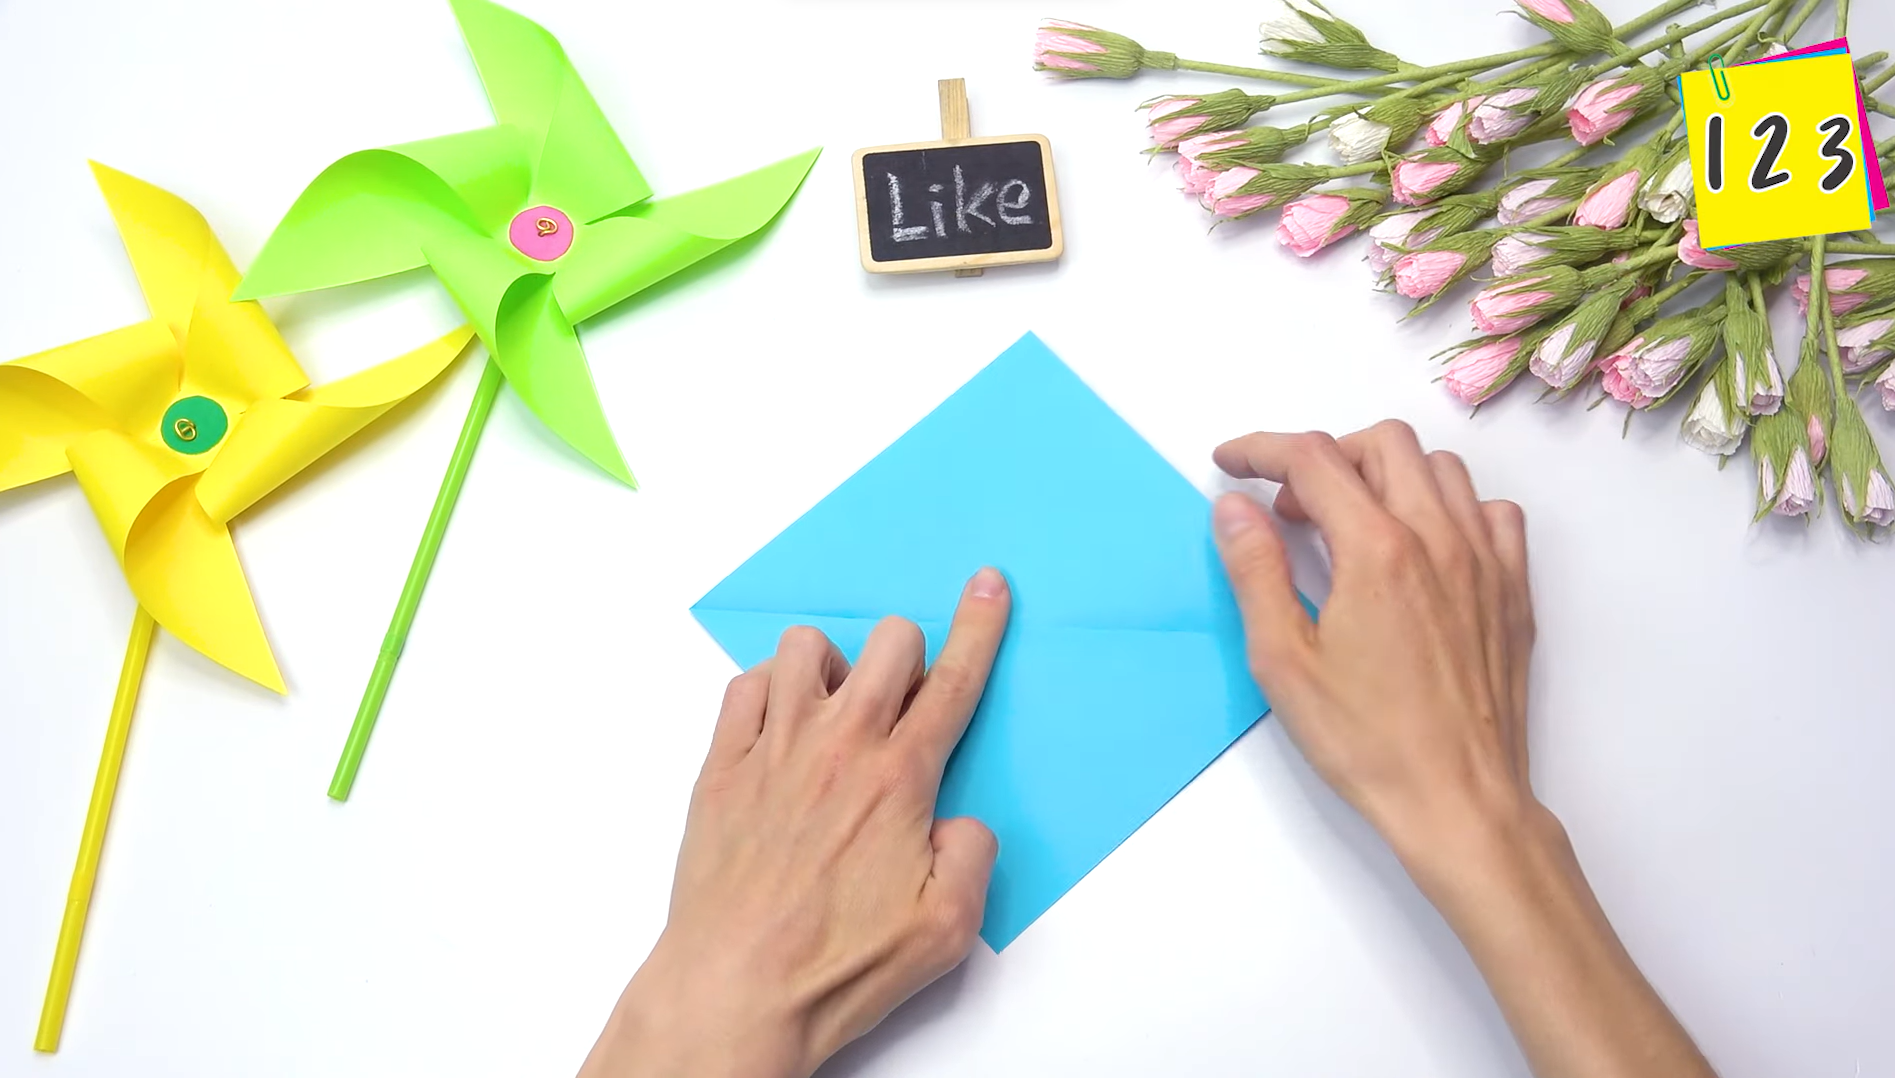
\includegraphics[width= 0.7\linewidth]{2b}
		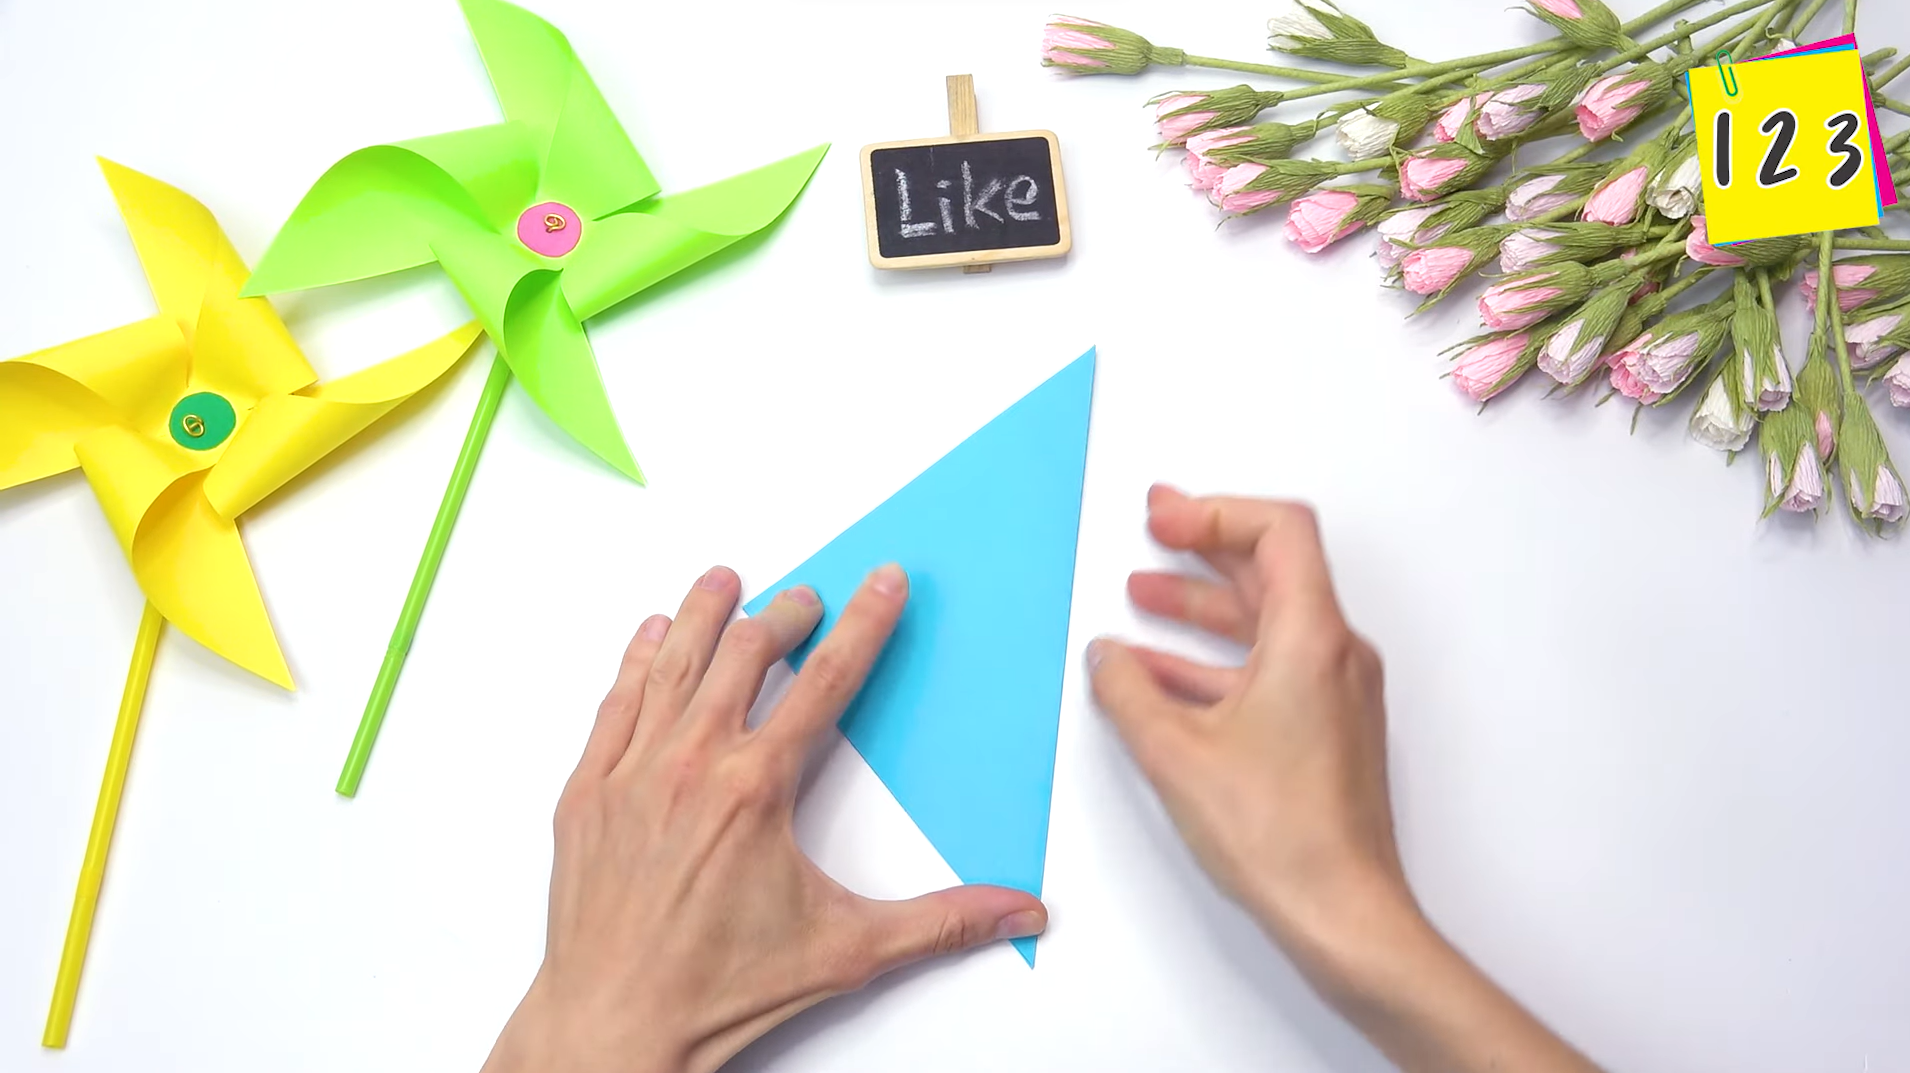
\includegraphics[width= 0.7\linewidth]{2c}
		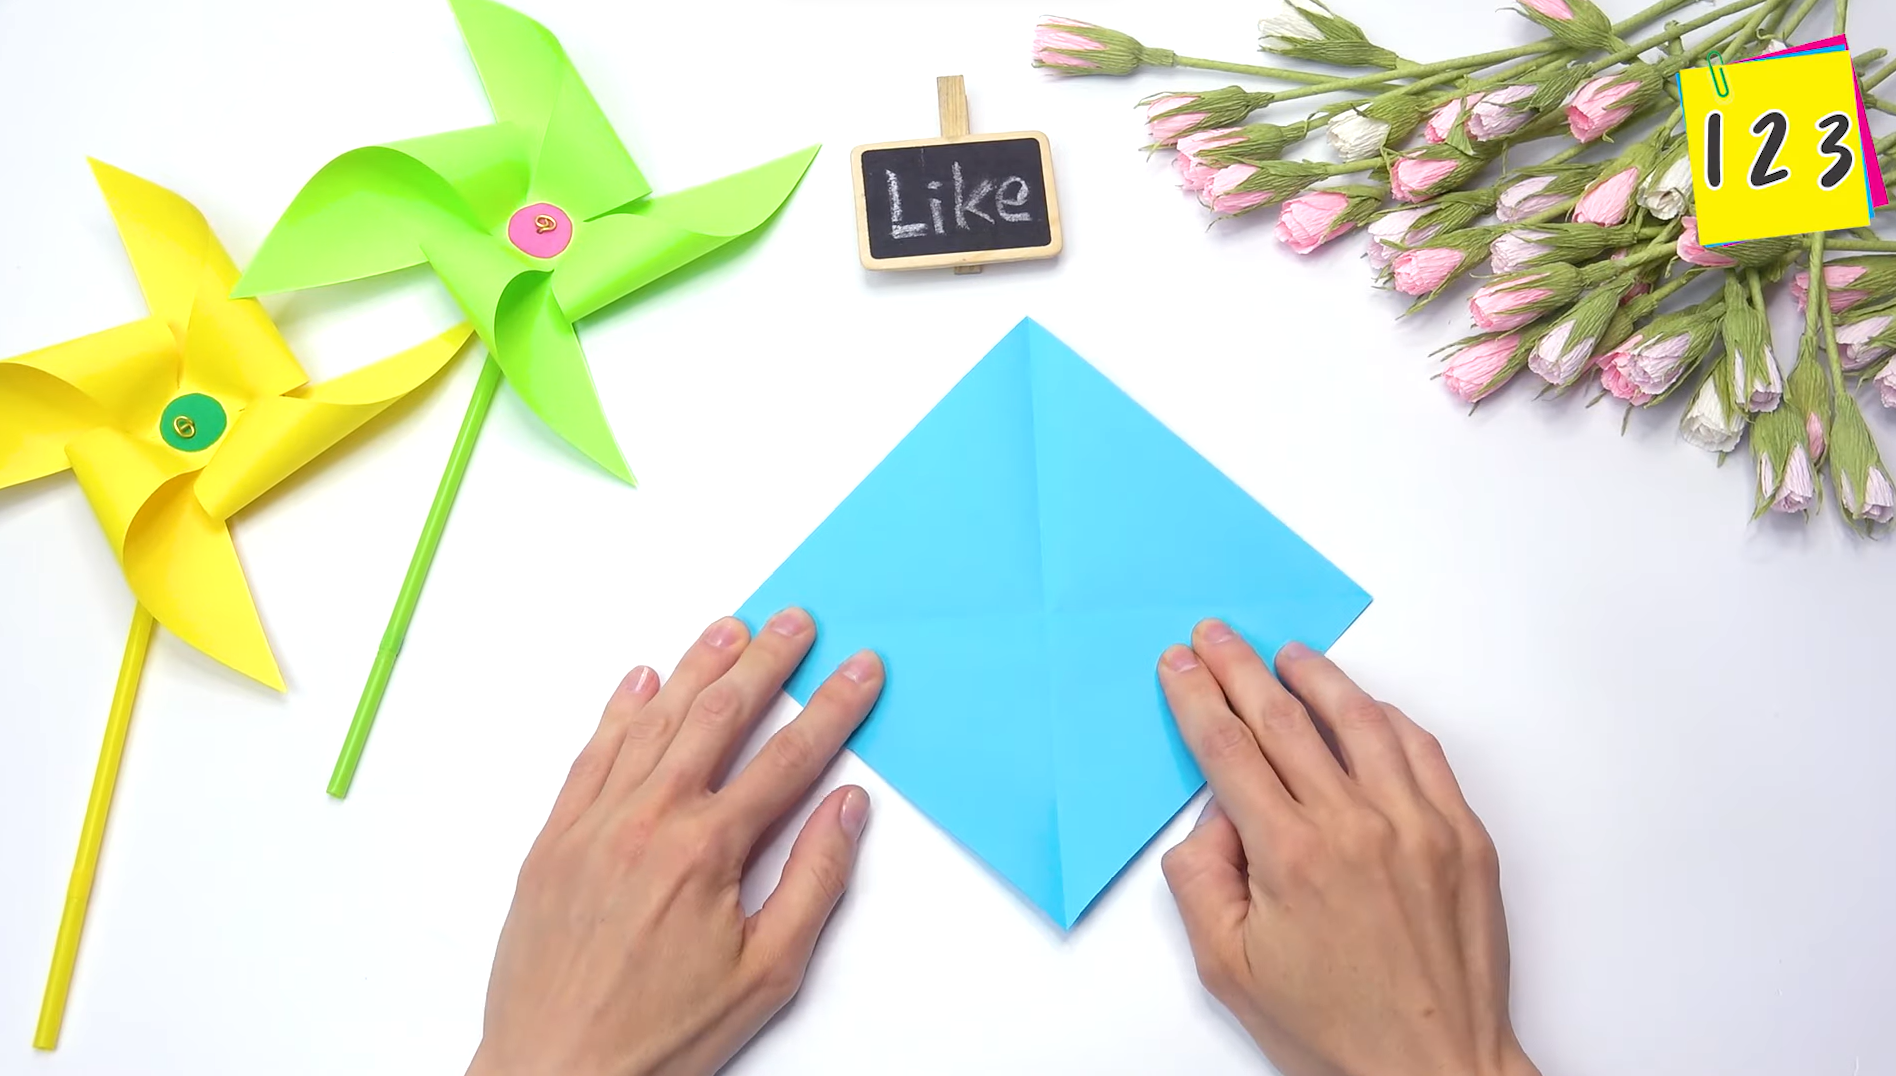
\includegraphics[width= 0.7\linewidth]{2d}
		\vspace*{-10pt}
	\end{figure}
	\textit{Bước $3$:} Dùng thước và bút chì đánh dấu tâm của hình vuông và $8$ đoạn thẳng trên hai đường chéo của hình vuông (mỗi đoạn dài $1,5$cm).
	\begin{figure}[H]
		\vspace*{-5pt}
		\centering
		\captionsetup{labelformat= empty, justification=centering}
		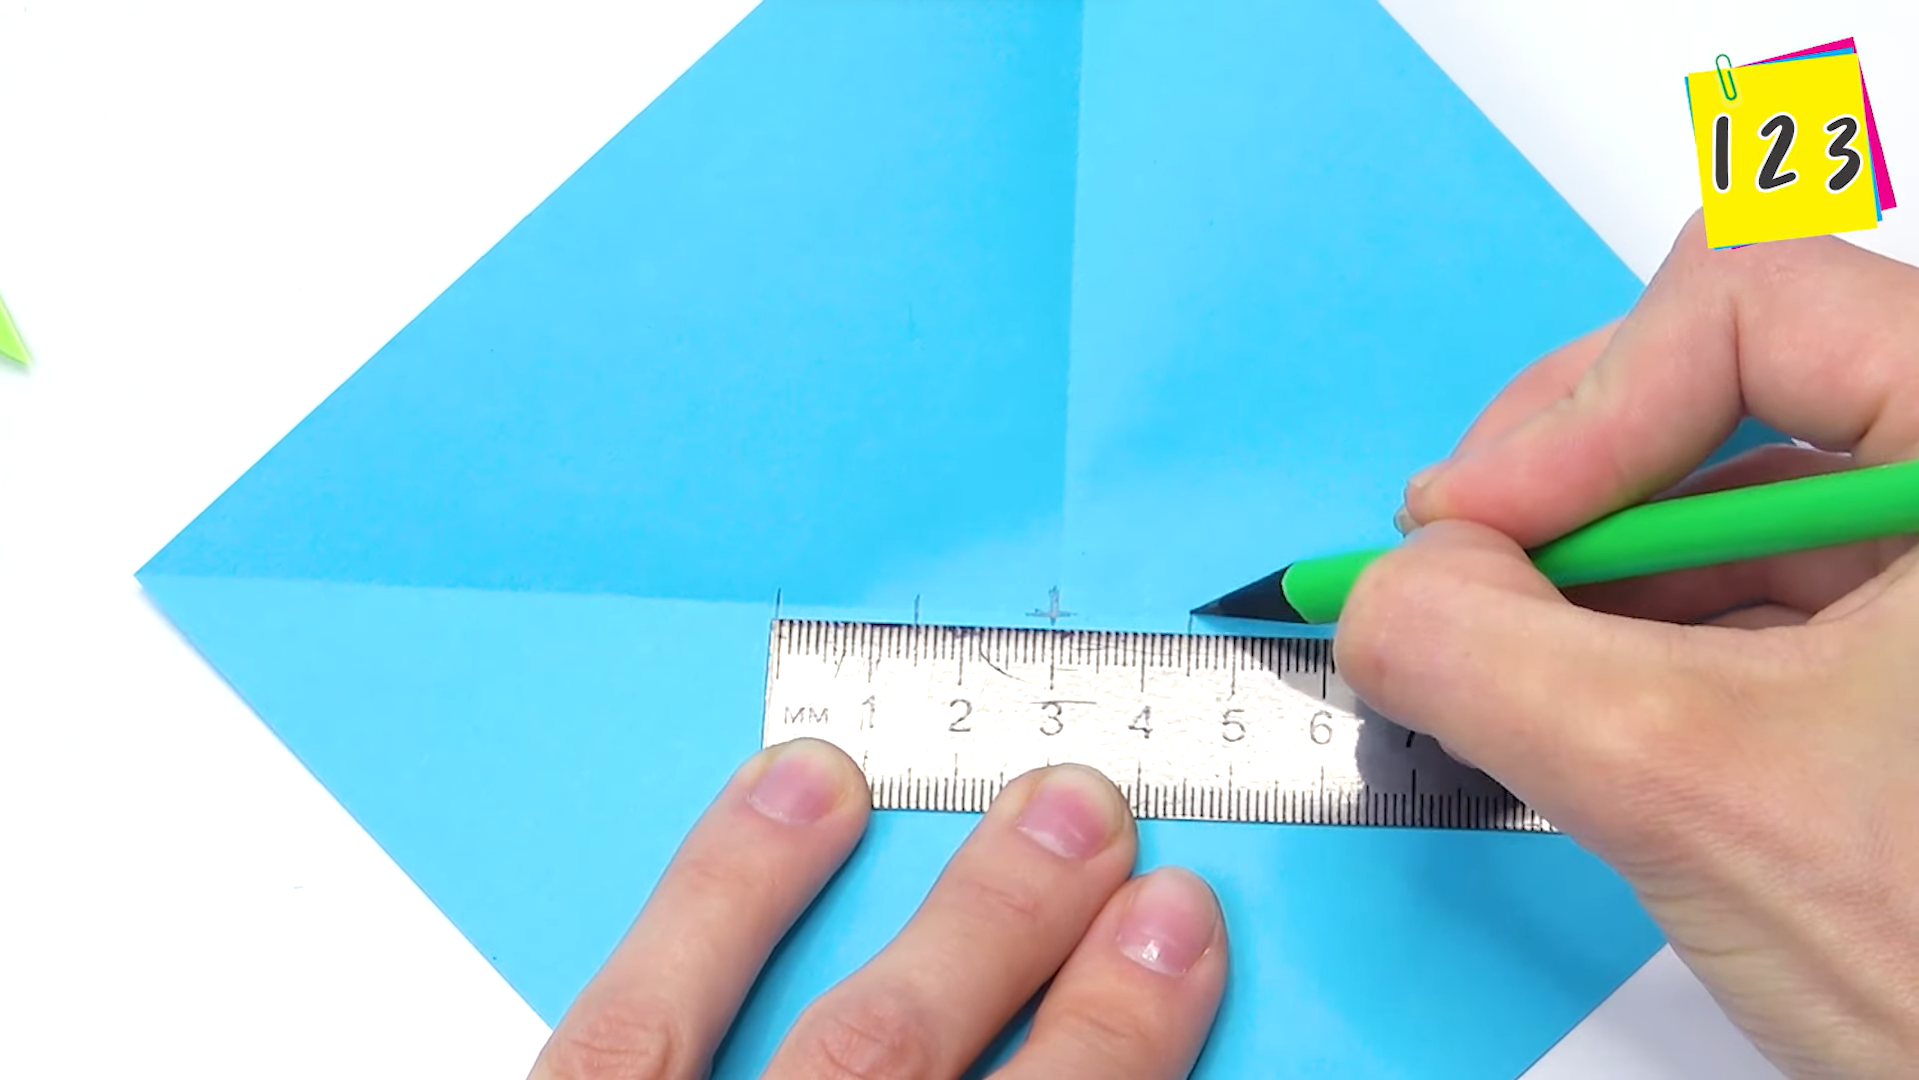
\includegraphics[width= 0.7\linewidth]{3a}
%		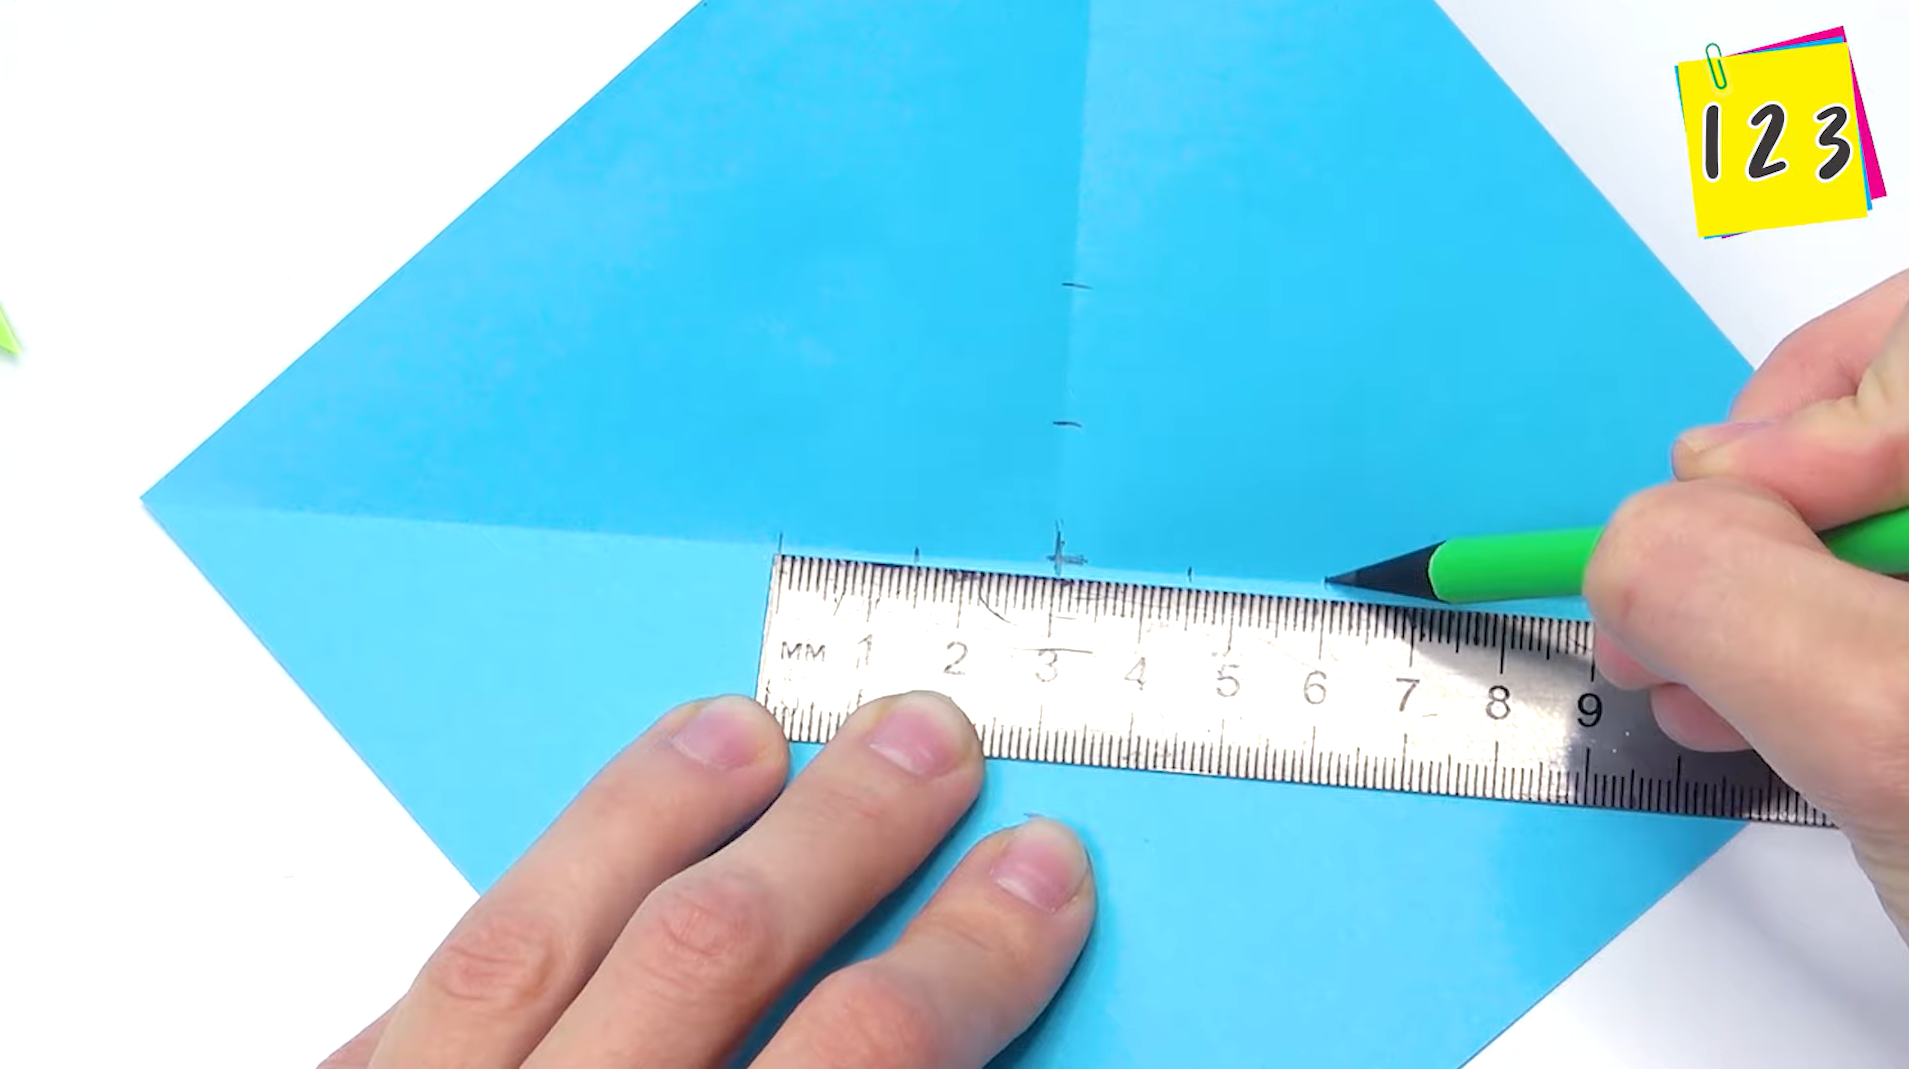
\includegraphics[width= 1\linewidth]{3b}
%		\vspace*{-5pt}
	\end{figure}
\begin{figure}[H]
	\vspace*{5pt}
	\centering
	\captionsetup{labelformat= empty, justification=centering}
%	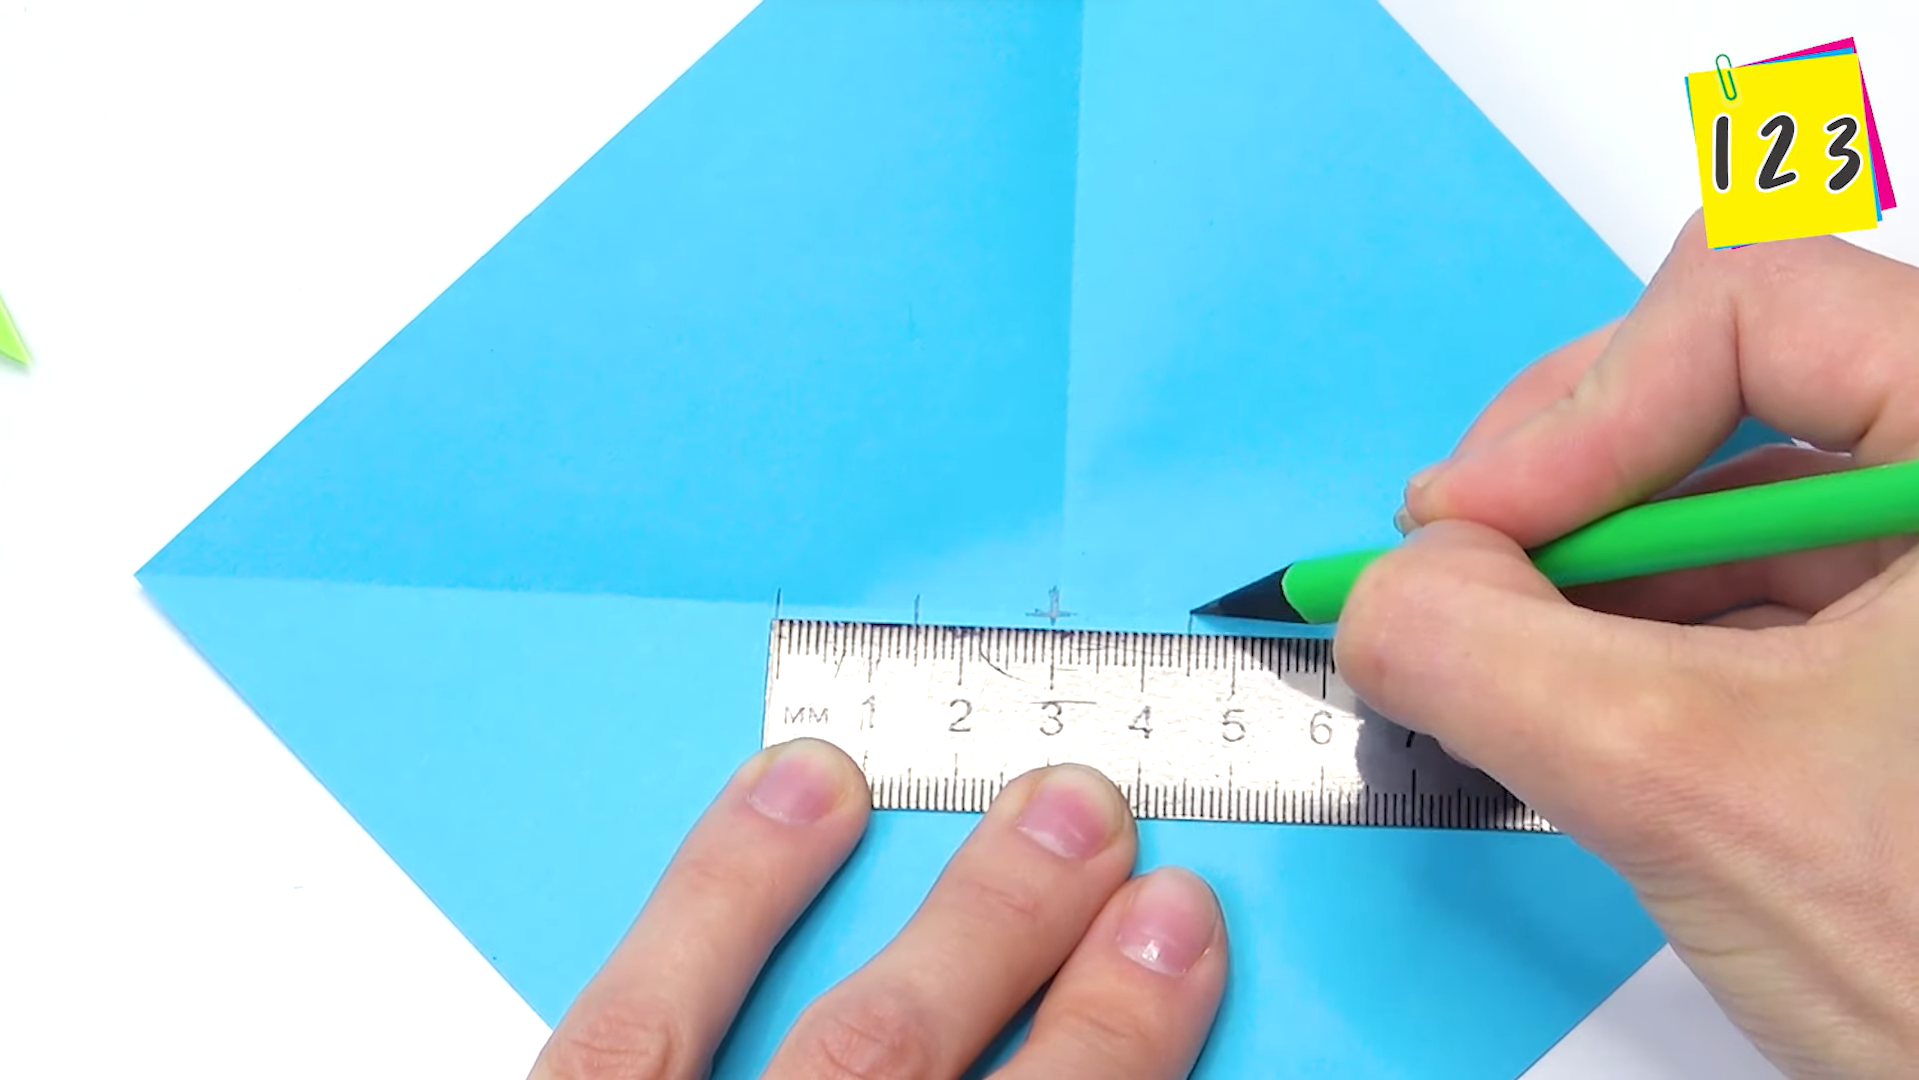
\includegraphics[width= 1\linewidth]{3a}
	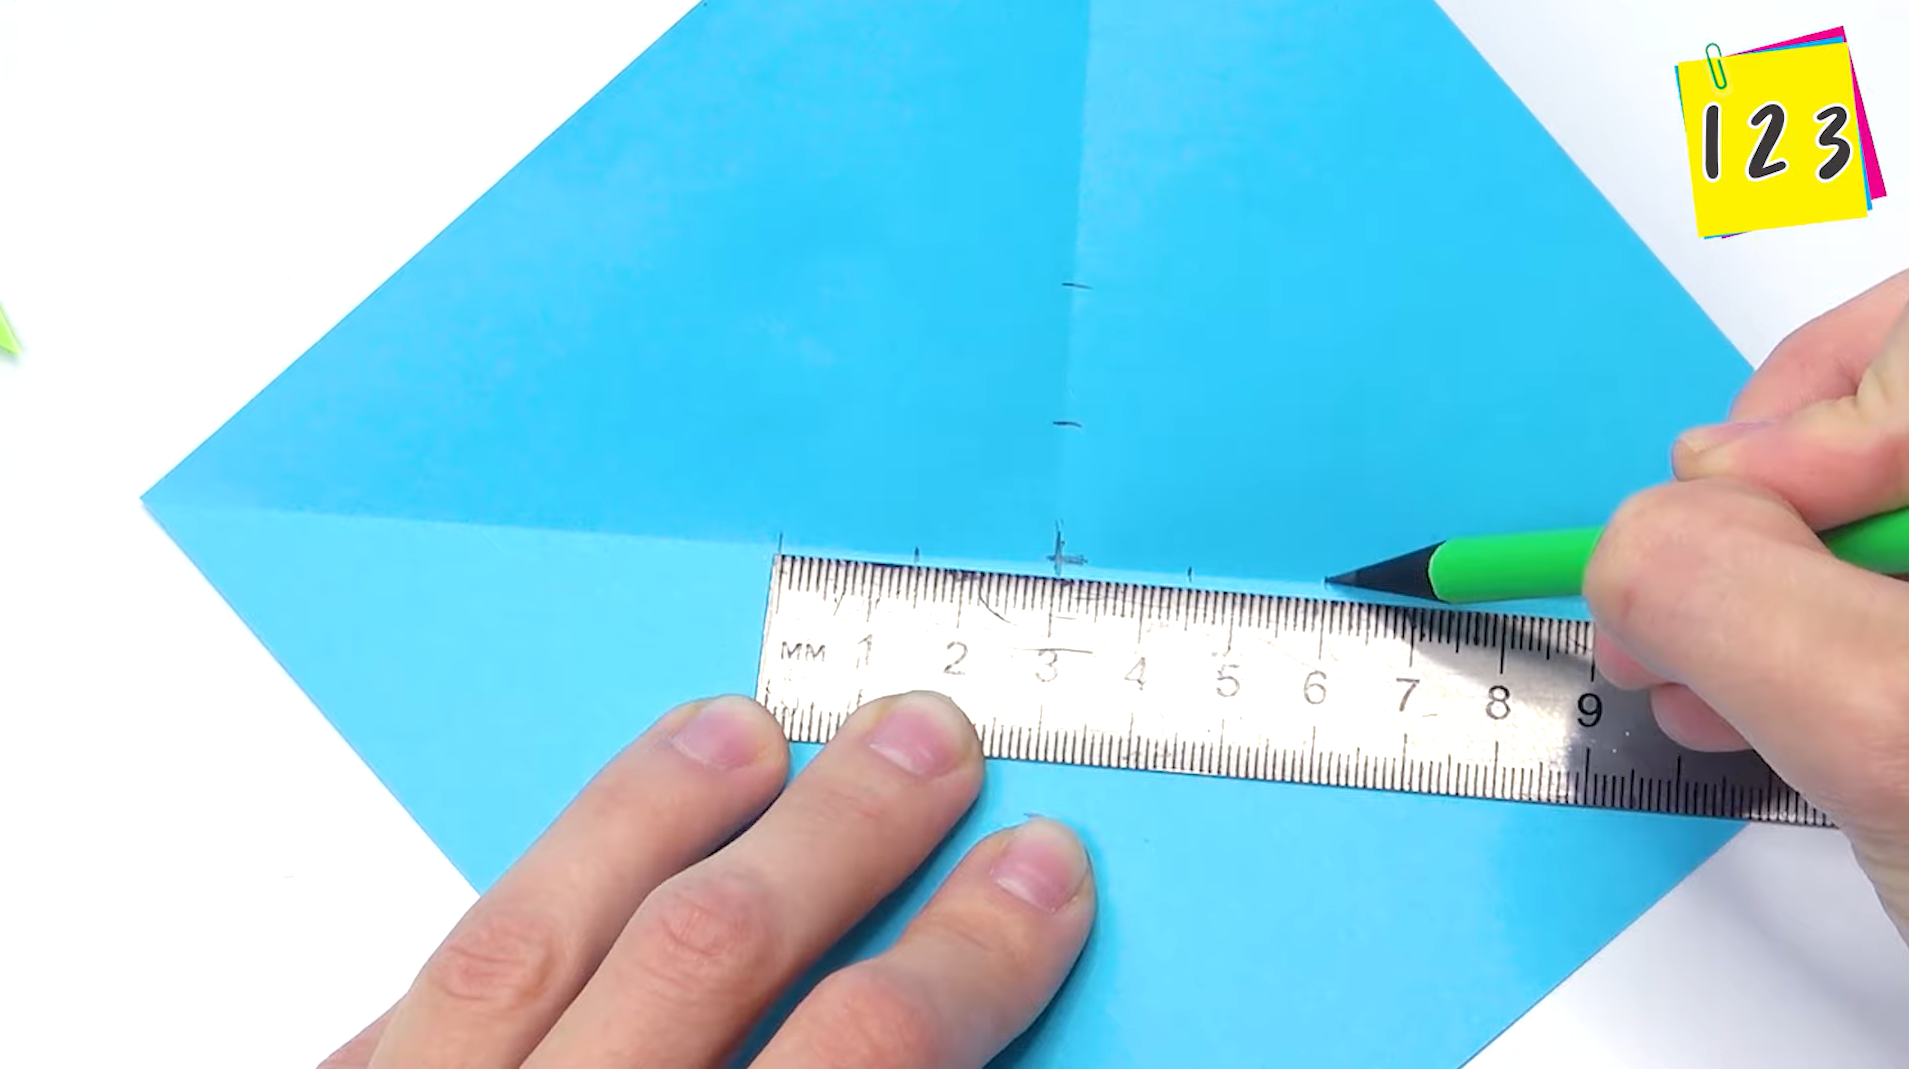
\includegraphics[width= 0.75\linewidth]{3b}
	\vspace*{-15pt}
\end{figure}
	\textit{Bước $4$:} Dùng kéo cắt các đường chéo của hình vuông như hình minh họa.
	\begin{figure}[H]
		\vspace*{-5pt}
		\centering
		\captionsetup{labelformat= empty, justification=centering}
		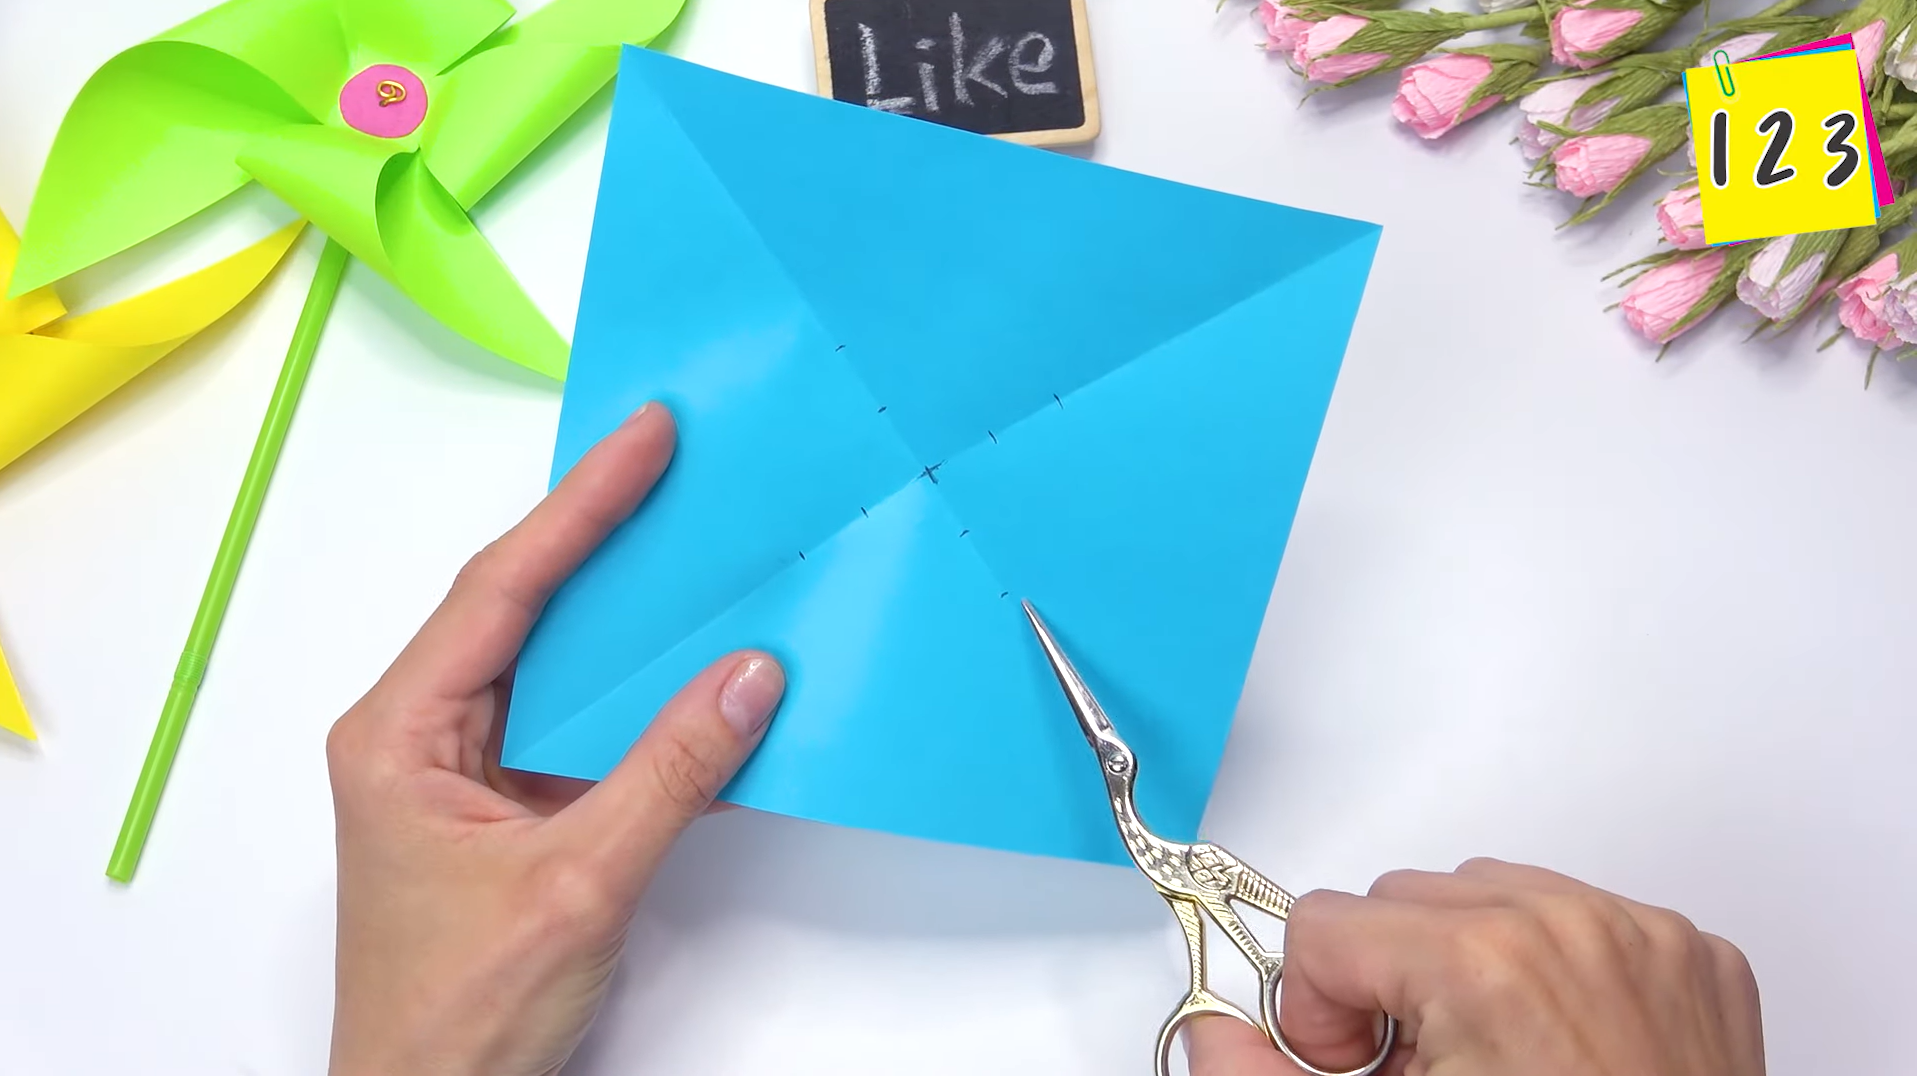
\includegraphics[width= 0.75\linewidth]{4a}
		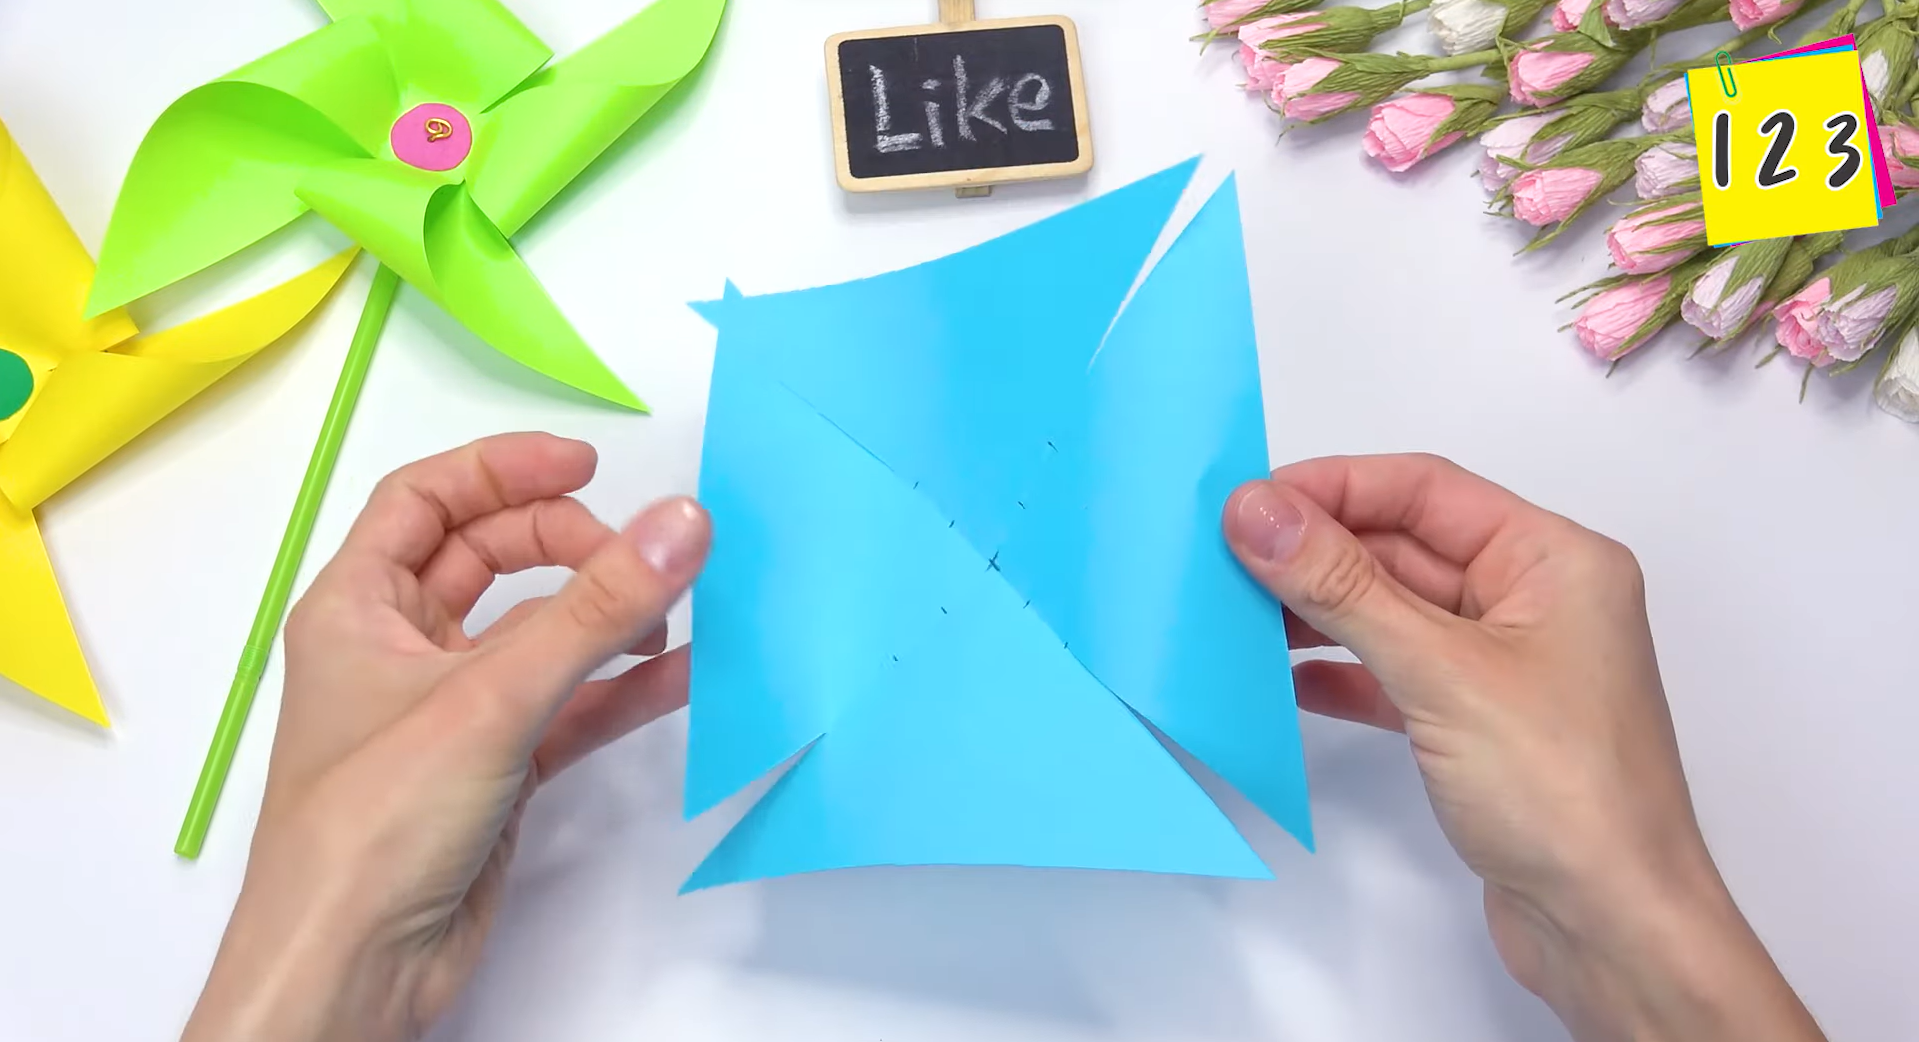
\includegraphics[width= 0.75\linewidth]{4b}
		\vspace*{-15pt}
	\end{figure}
	\textit{Bước $5$:} Sử dụng hồ dán để dán các góc của hình vuông như hình minh họa nhằm tạo ra các cánh của chong chóng.
	\begin{figure}[H]
		\vspace*{-5pt}
		\centering
		\captionsetup{labelformat= empty, justification=centering}
		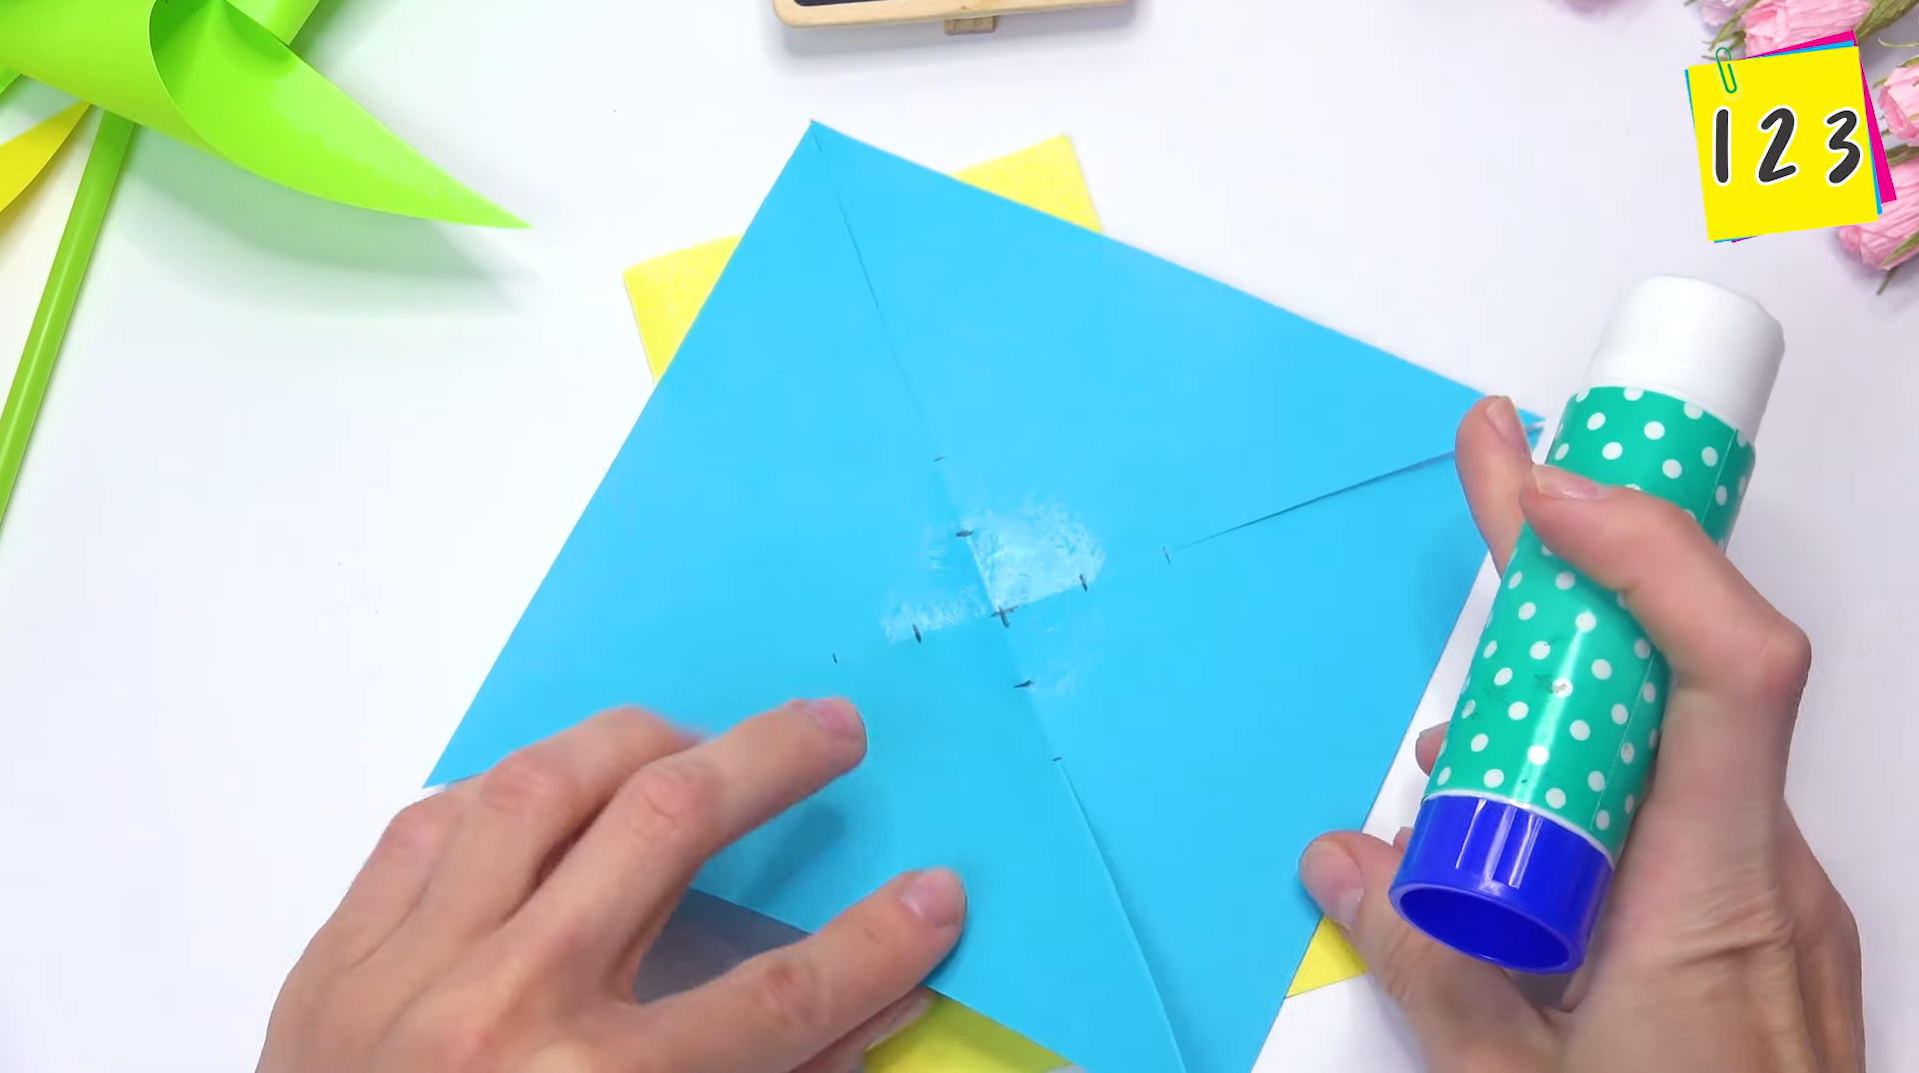
\includegraphics[width= 0.75\linewidth]{5a}
		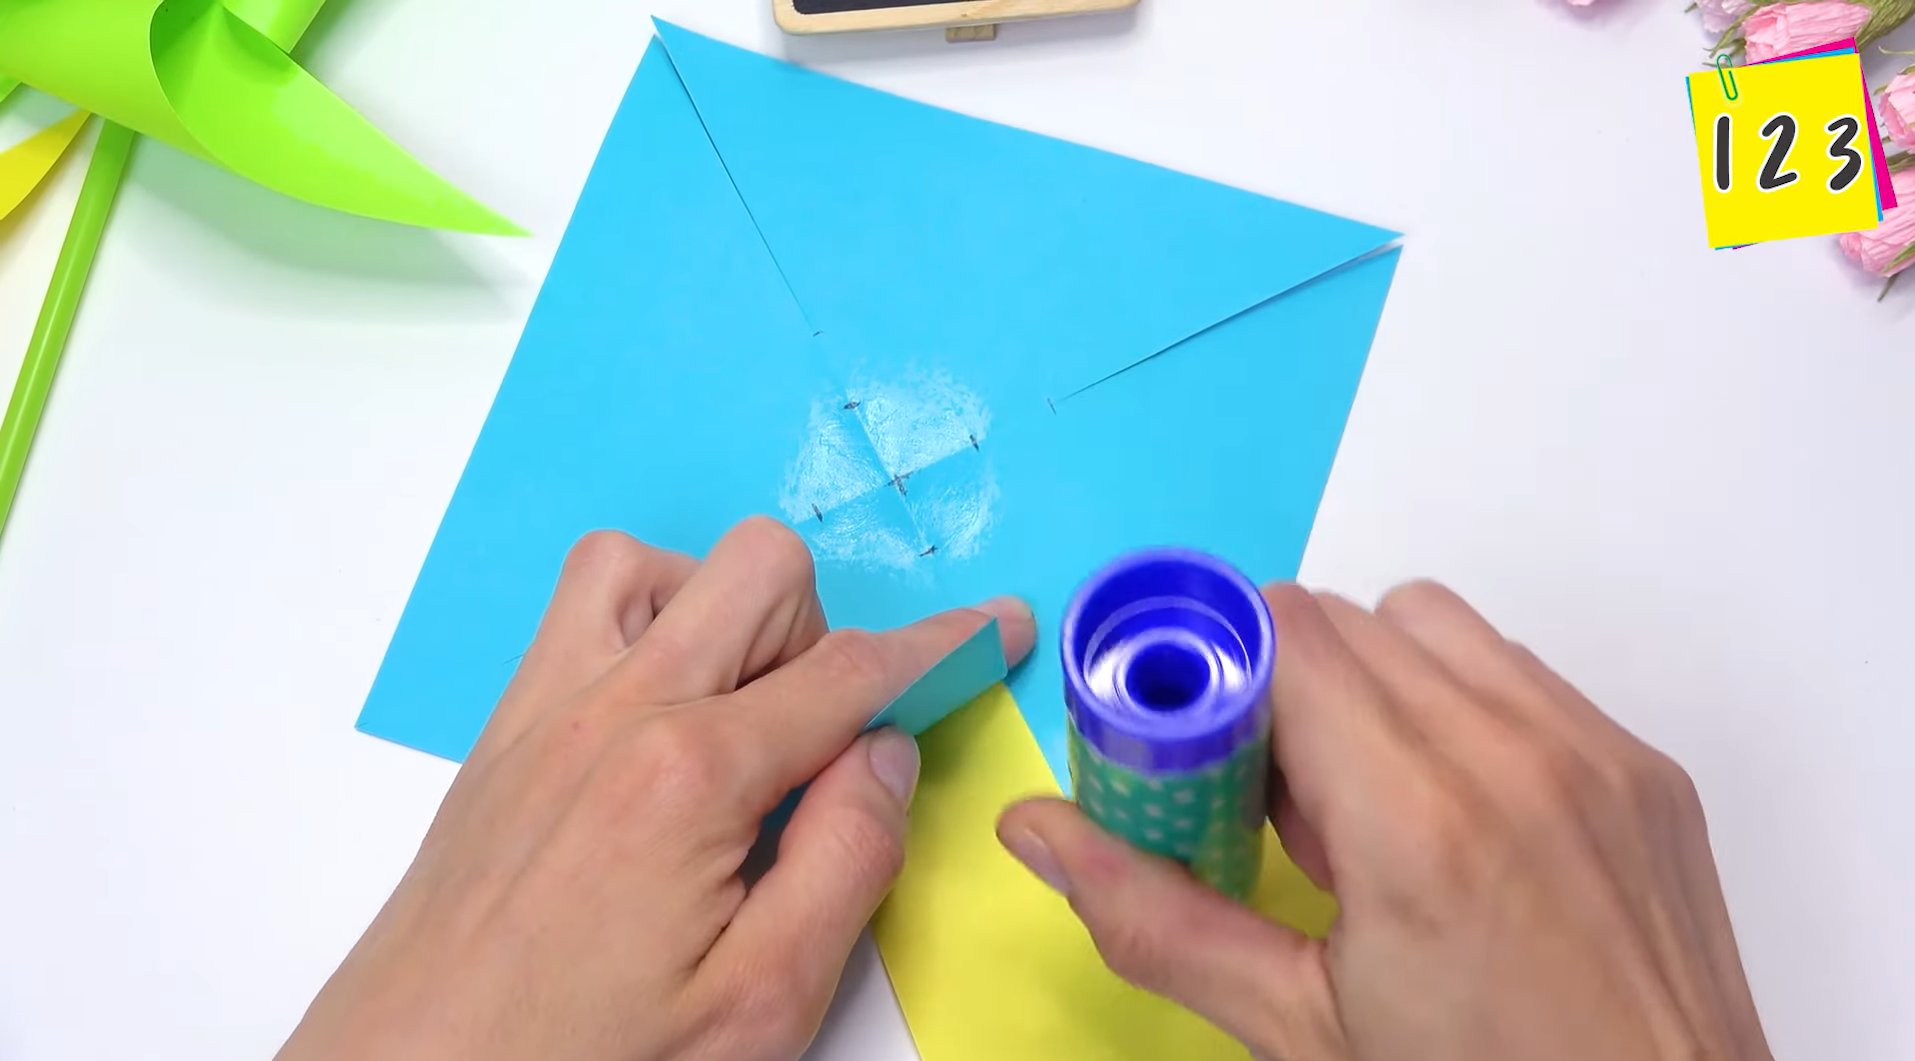
\includegraphics[width= 0.75\linewidth]{5b}
		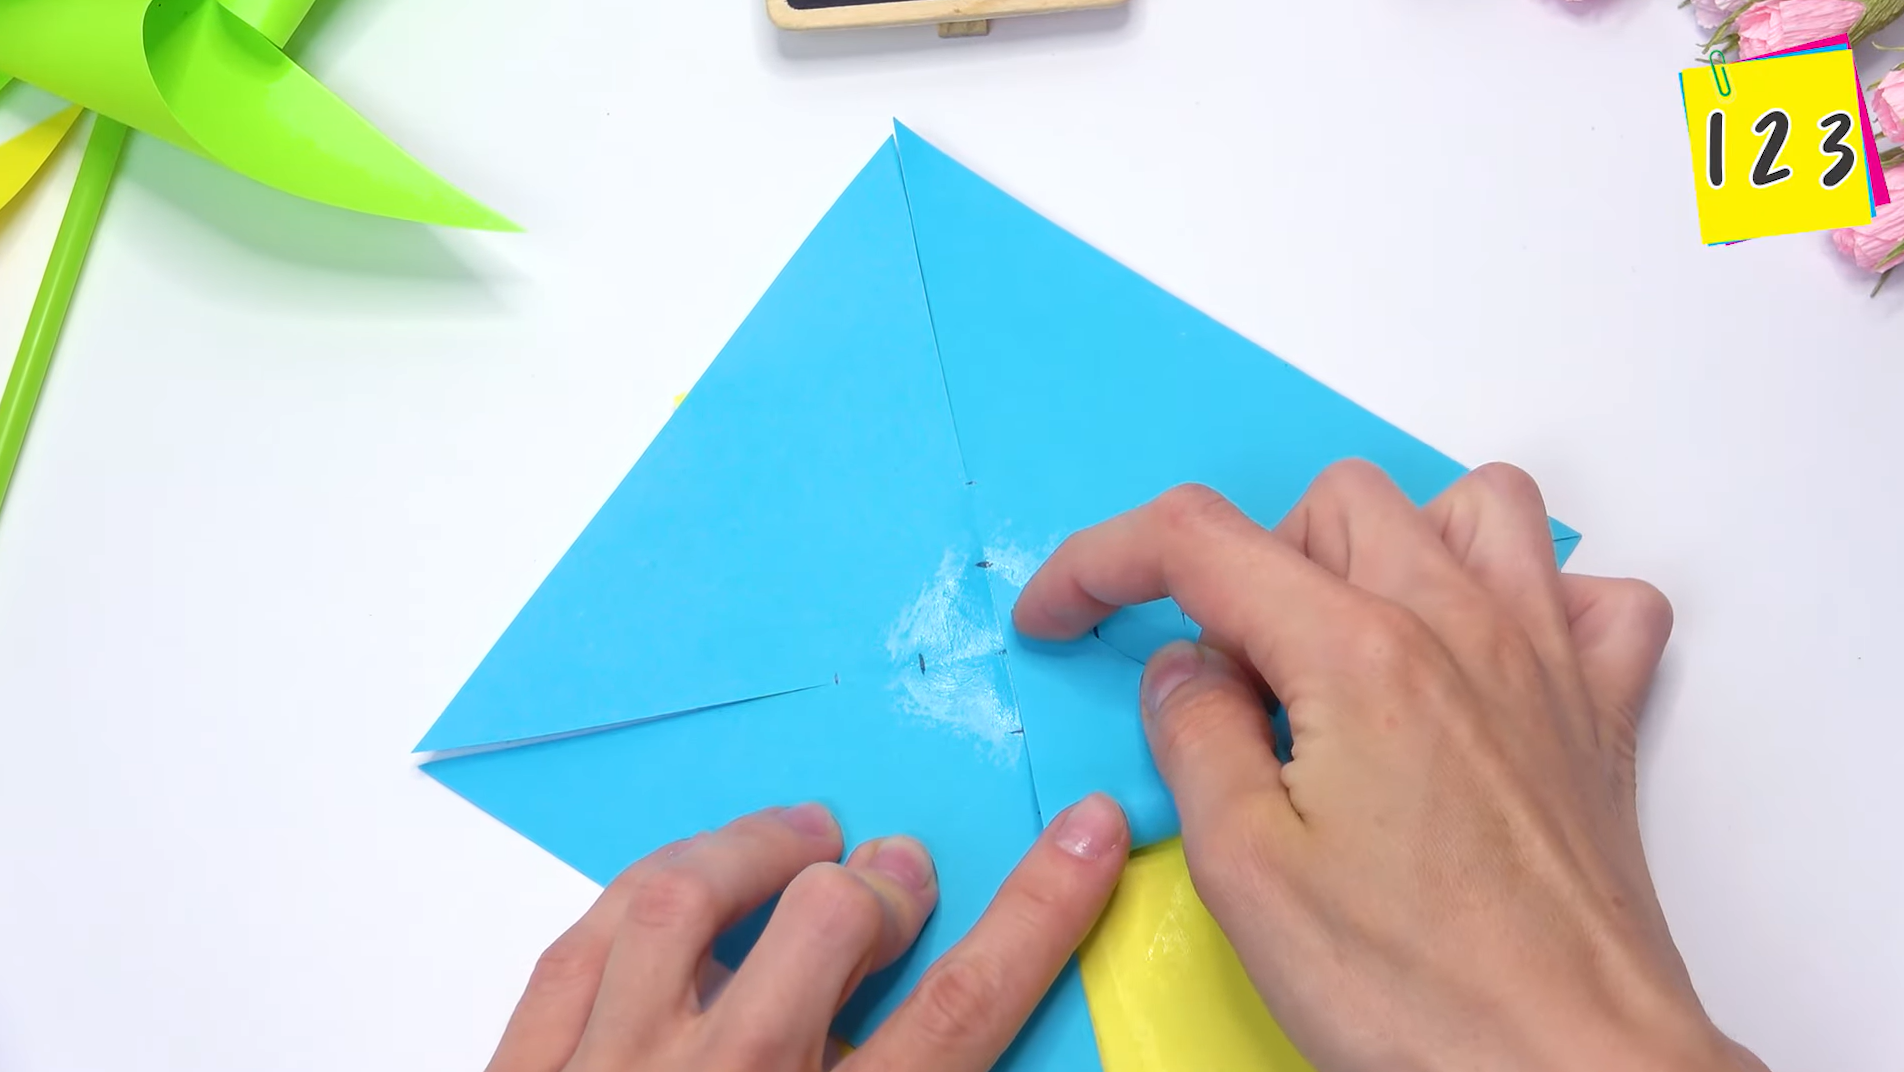
\includegraphics[width= 0.75\linewidth]{5c}
%		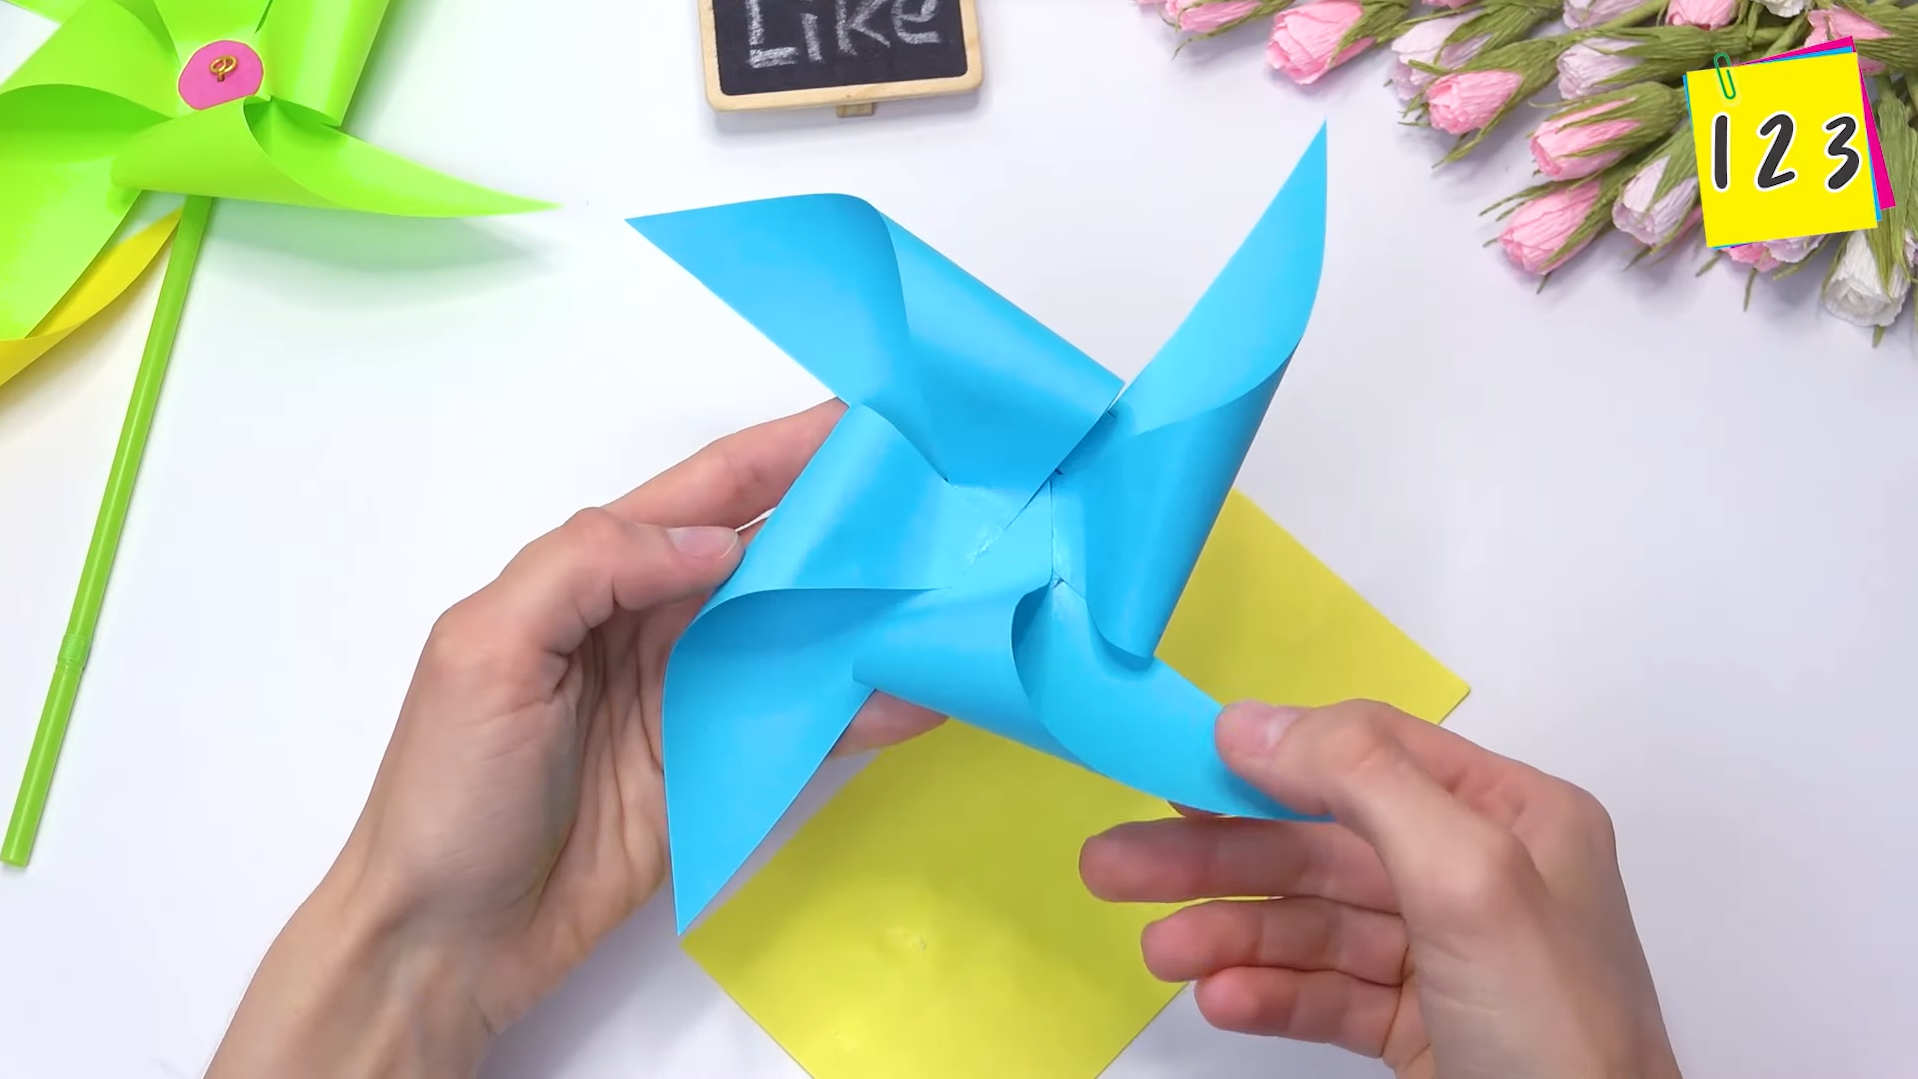
\includegraphics[width= 0.75\linewidth]{5d}
		\vspace*{-5pt}
	\end{figure}
\begin{figure}[H]
	\vspace*{5pt}
	\centering
	\captionsetup{labelformat= empty, justification=centering}
%	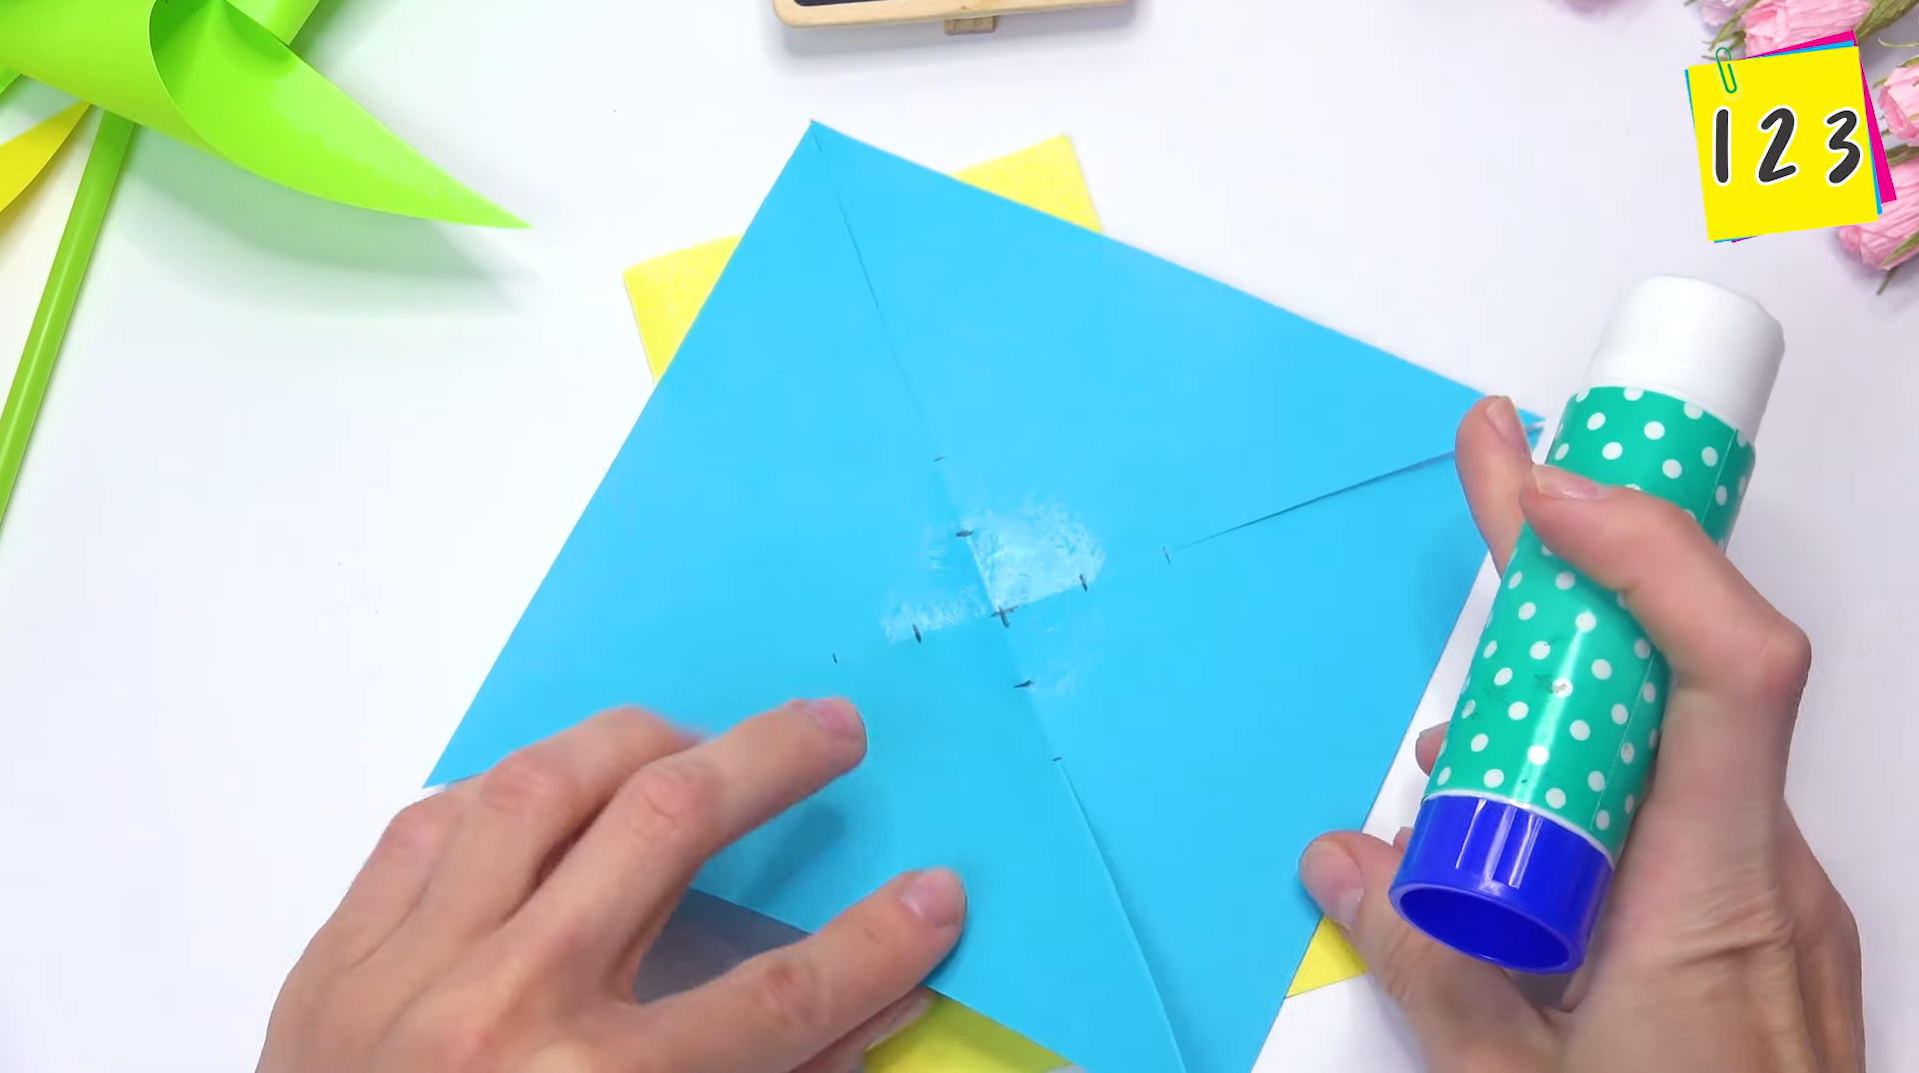
\includegraphics[width= 0.75\linewidth]{5a}
%	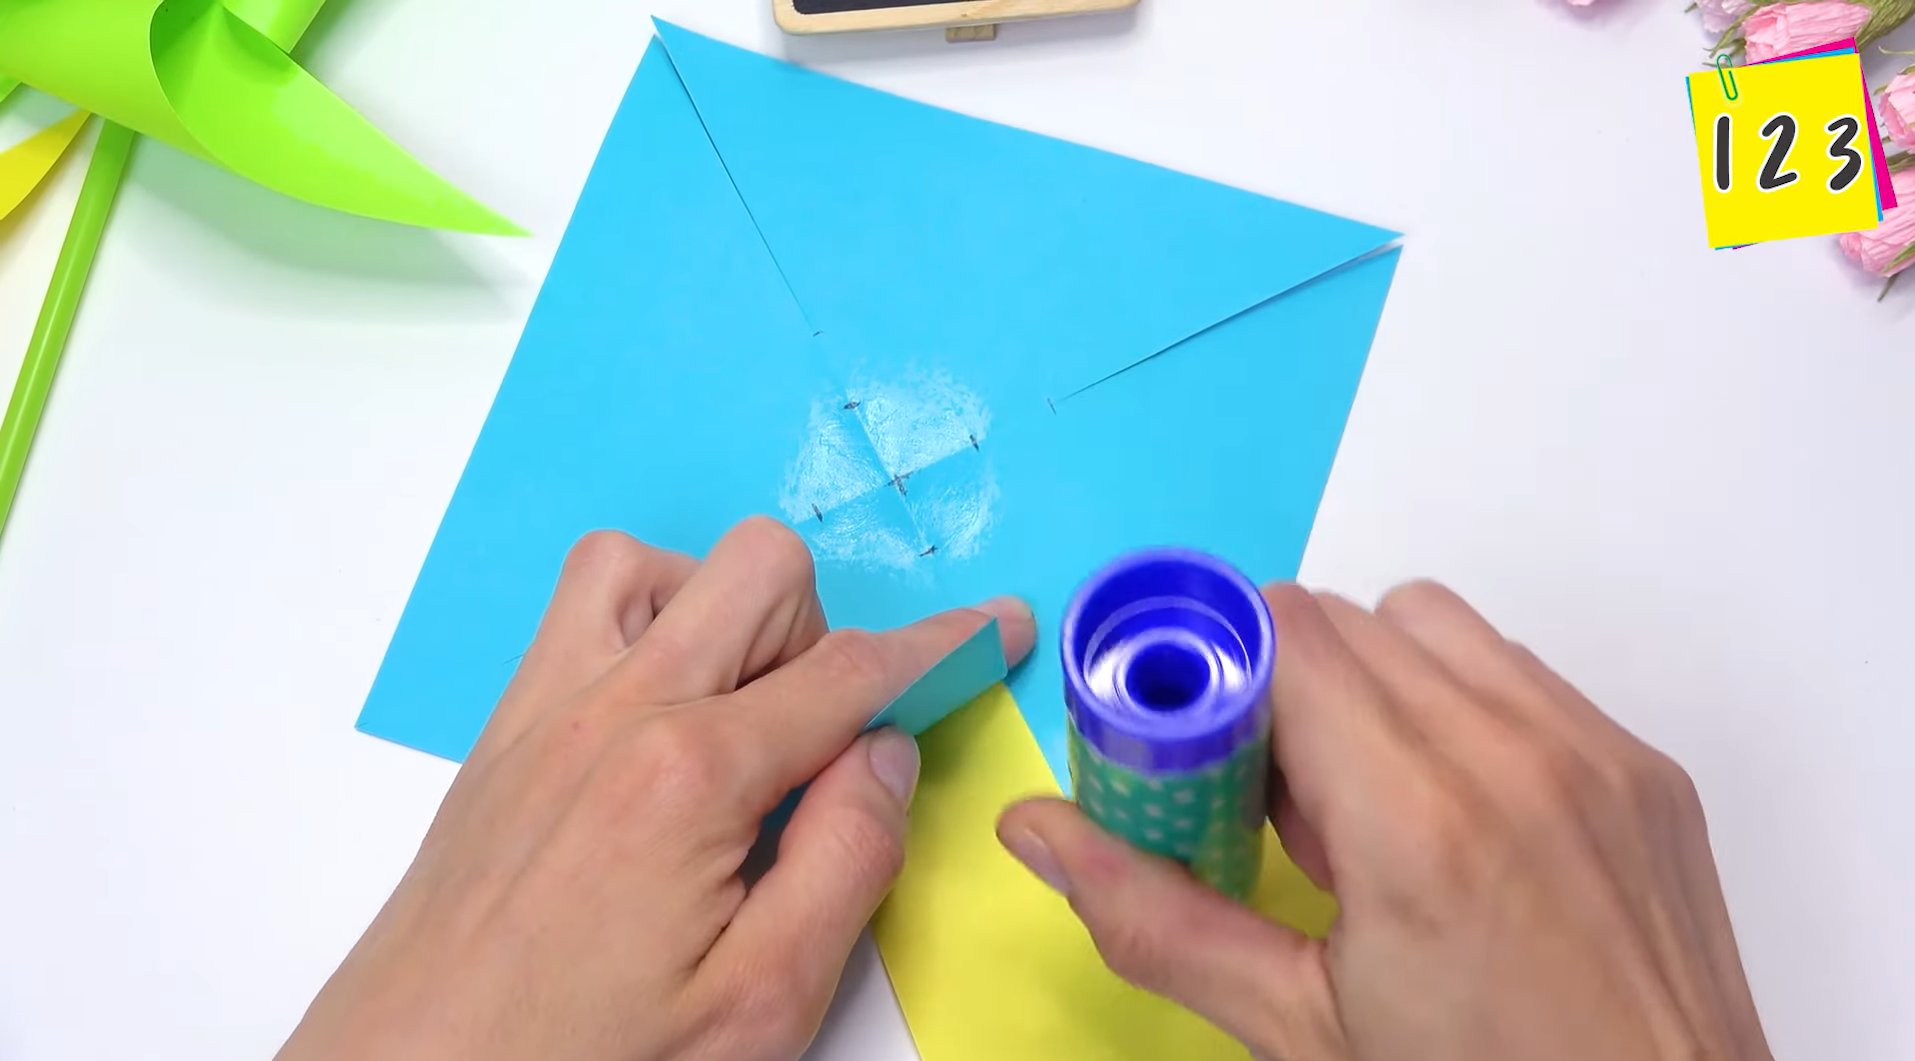
\includegraphics[width= 0.75\linewidth]{5b}
%	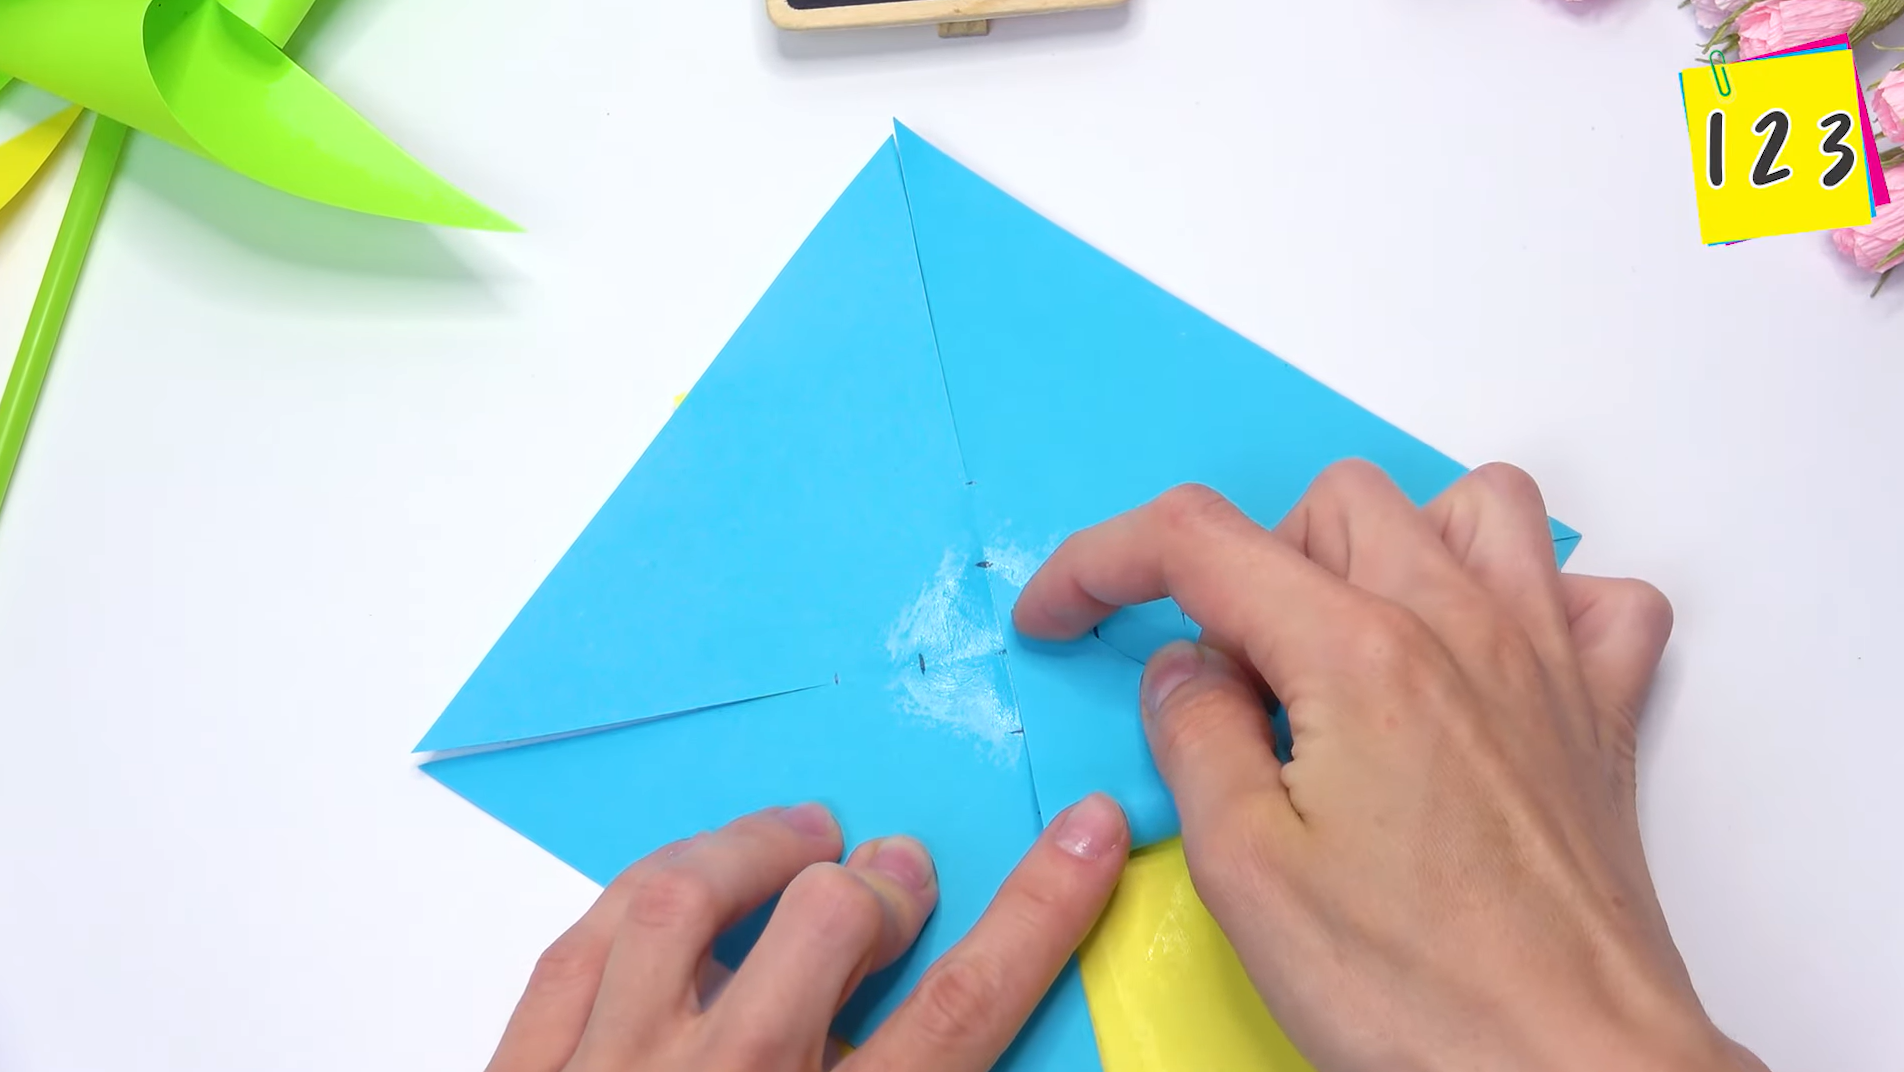
\includegraphics[width= 0.75\linewidth]{5c}
	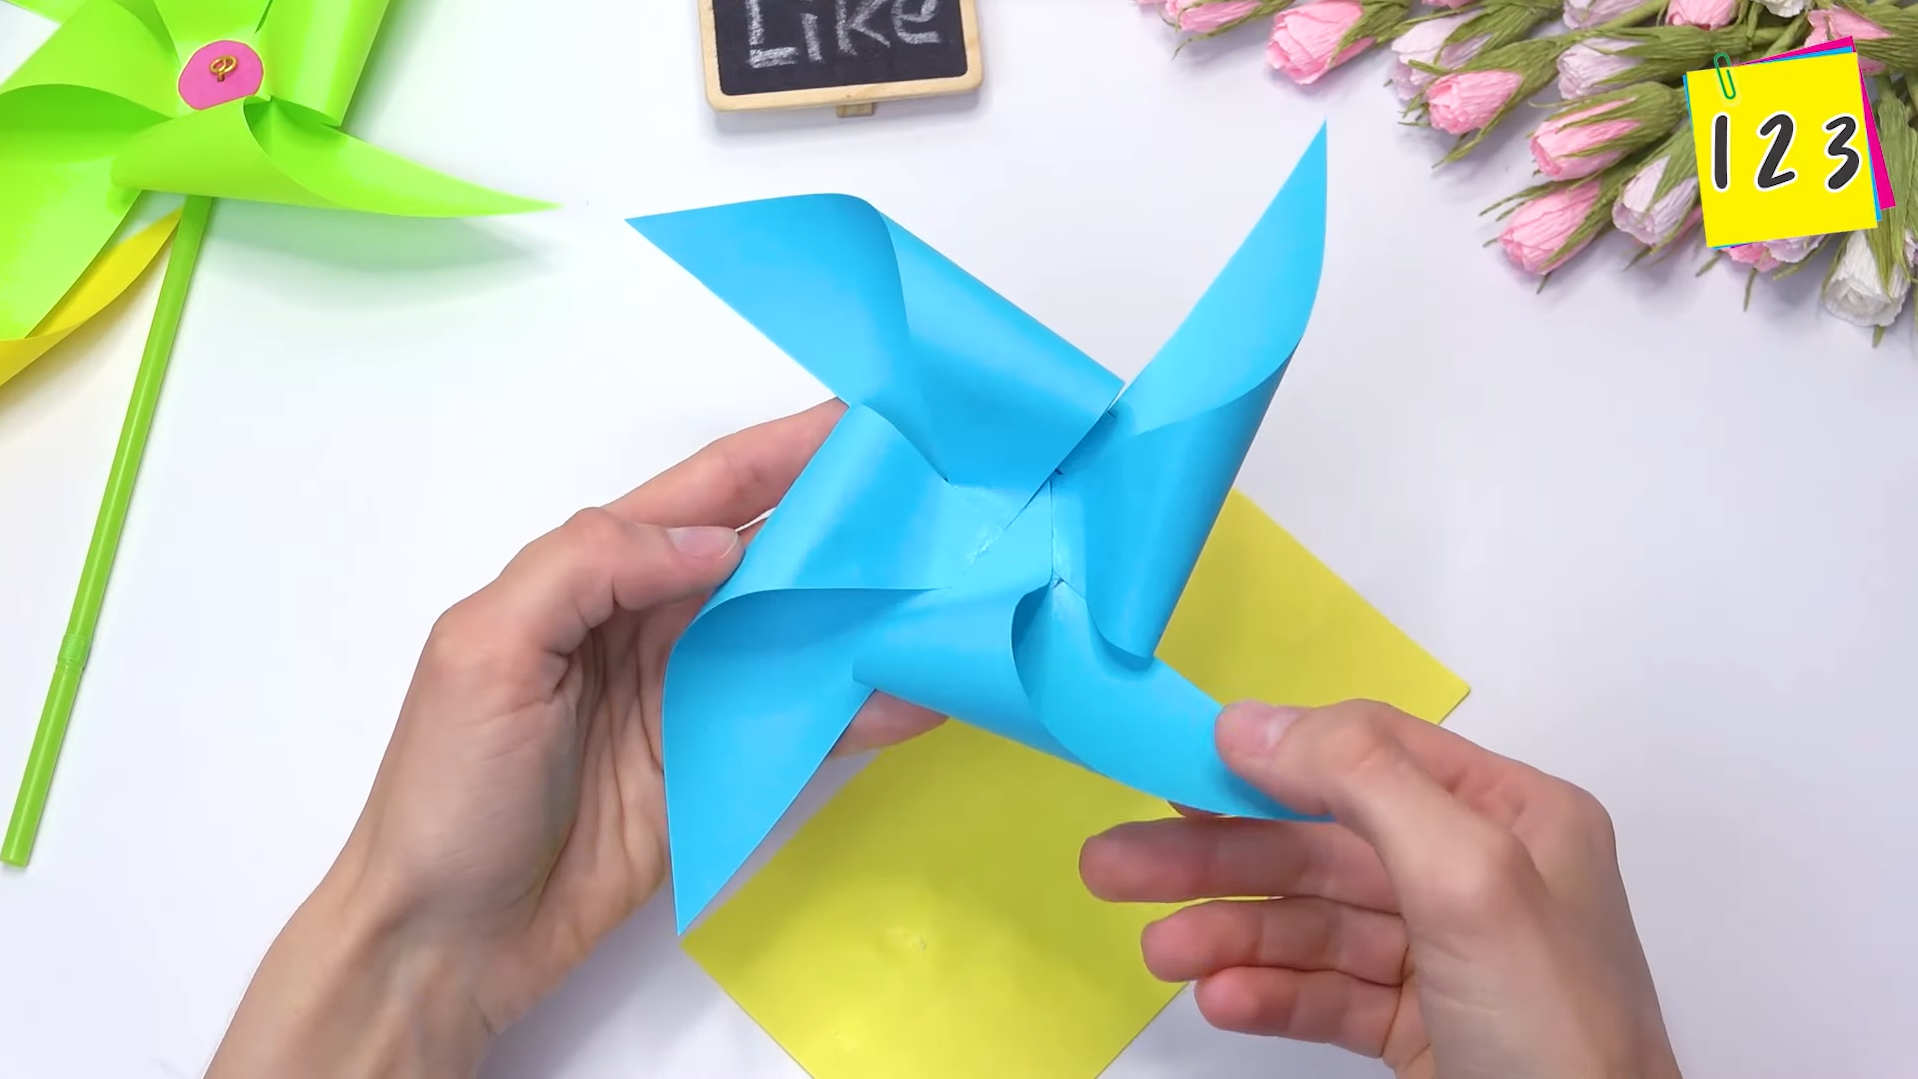
\includegraphics[width= 0.75\linewidth]{5d}
	\vspace*{-10pt}
\end{figure}
	\textit{Bước $6$:} Sử dụng com--pa hoặc thước có sẵn hình tròn để vẽ một hình tròn rồi dùng kéo cắt hình tròn đó ra. Sau đó dùng keo dán hình tròn lên chính giữa chong chóng.
	\begin{figure}[H]
		\vspace*{-5pt}
		\centering
		\captionsetup{labelformat= empty, justification=centering}
		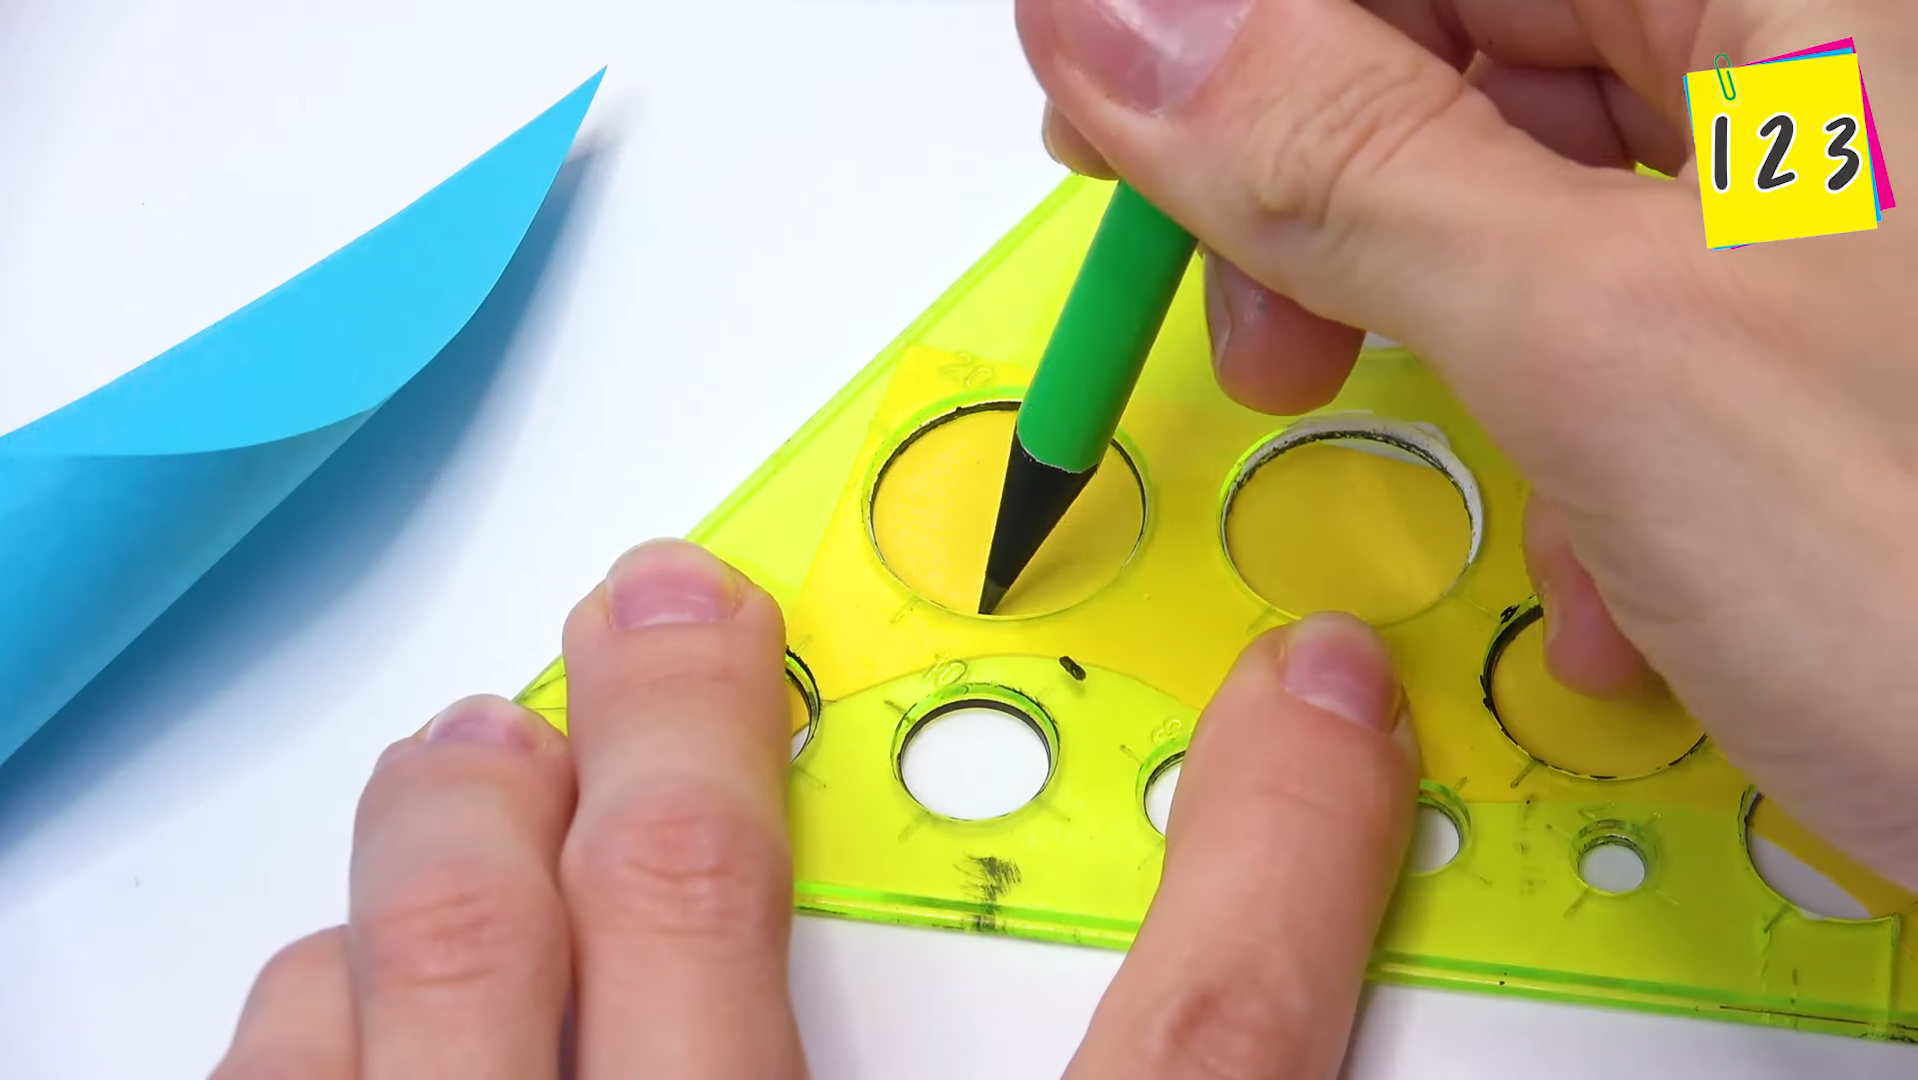
\includegraphics[width= 0.75\linewidth]{6a}
		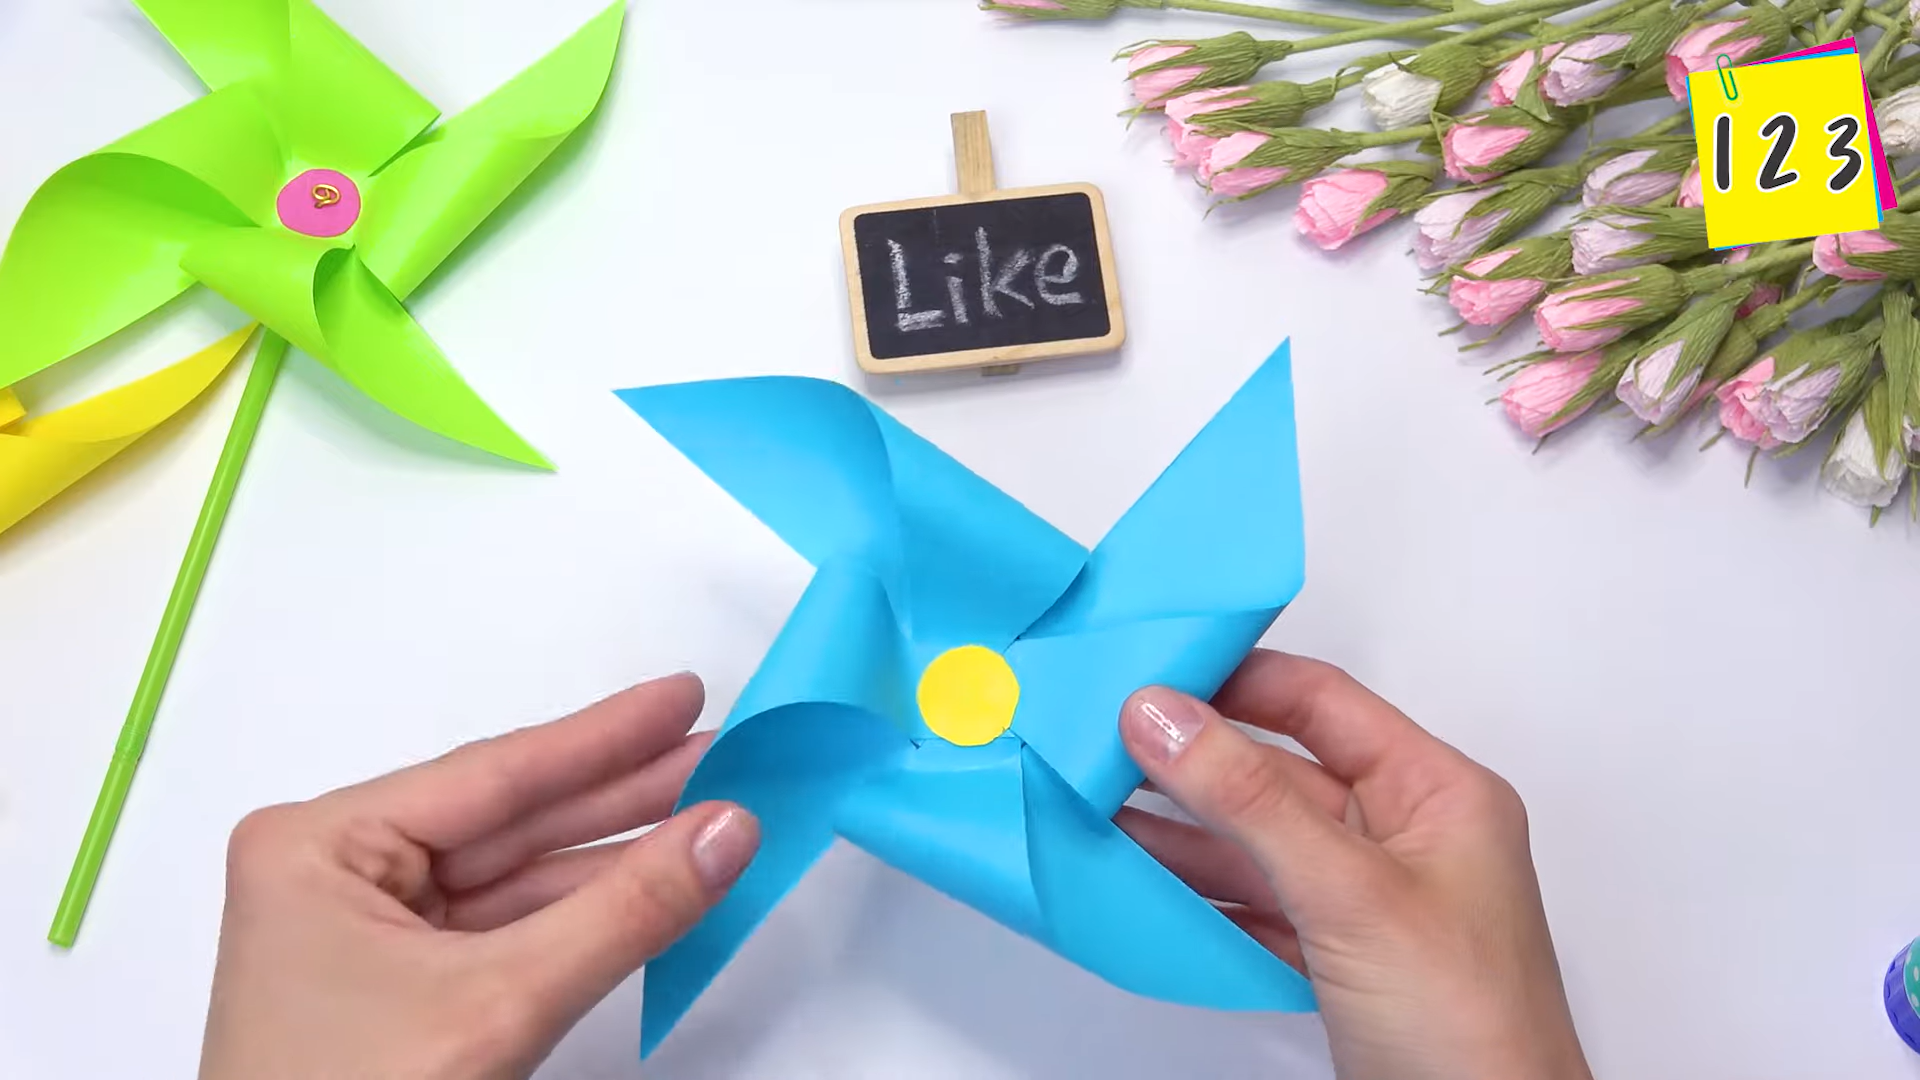
\includegraphics[width= 0.75\linewidth]{6b}
		\vspace*{-10pt}
	\end{figure}
	\textit{Bước $7$:} Dùng đầu nhọn của com-pa đâm một lỗ chính giữa vào hình tròn, xuyên qua chong chóng.
	\begin{figure}[H]
		\vspace*{-5pt}
		\centering
		\captionsetup{labelformat= empty, justification=centering}
		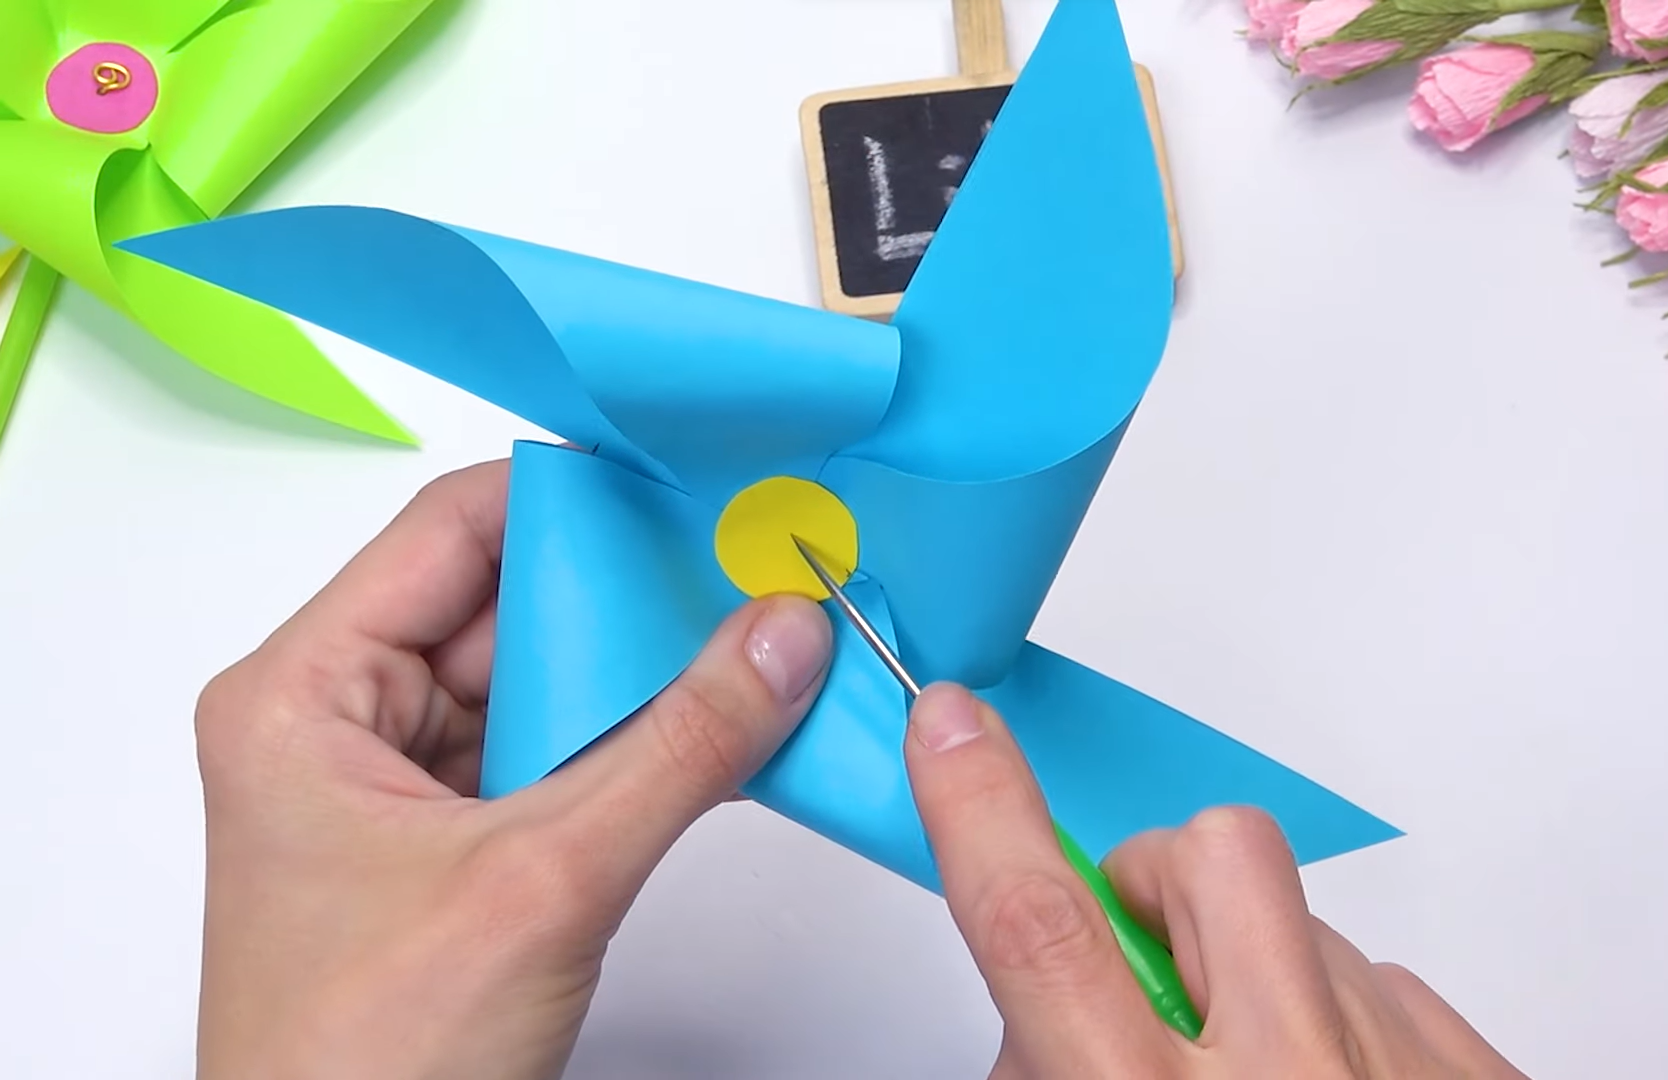
\includegraphics[width= 0.75\linewidth]{7}
		\vspace*{-10pt}
	\end{figure}
	\textit{Bước $8$:} Tiếp tục dùng đầu nhọn của com-pa đâm một lỗ vào ống hút nhựa (ống hút nhựa này sẽ là chiếc cán của chong chóng).
	\begin{figure}[H]
		\vspace*{-5pt}
		\centering
		\captionsetup{labelformat= empty, justification=centering}
		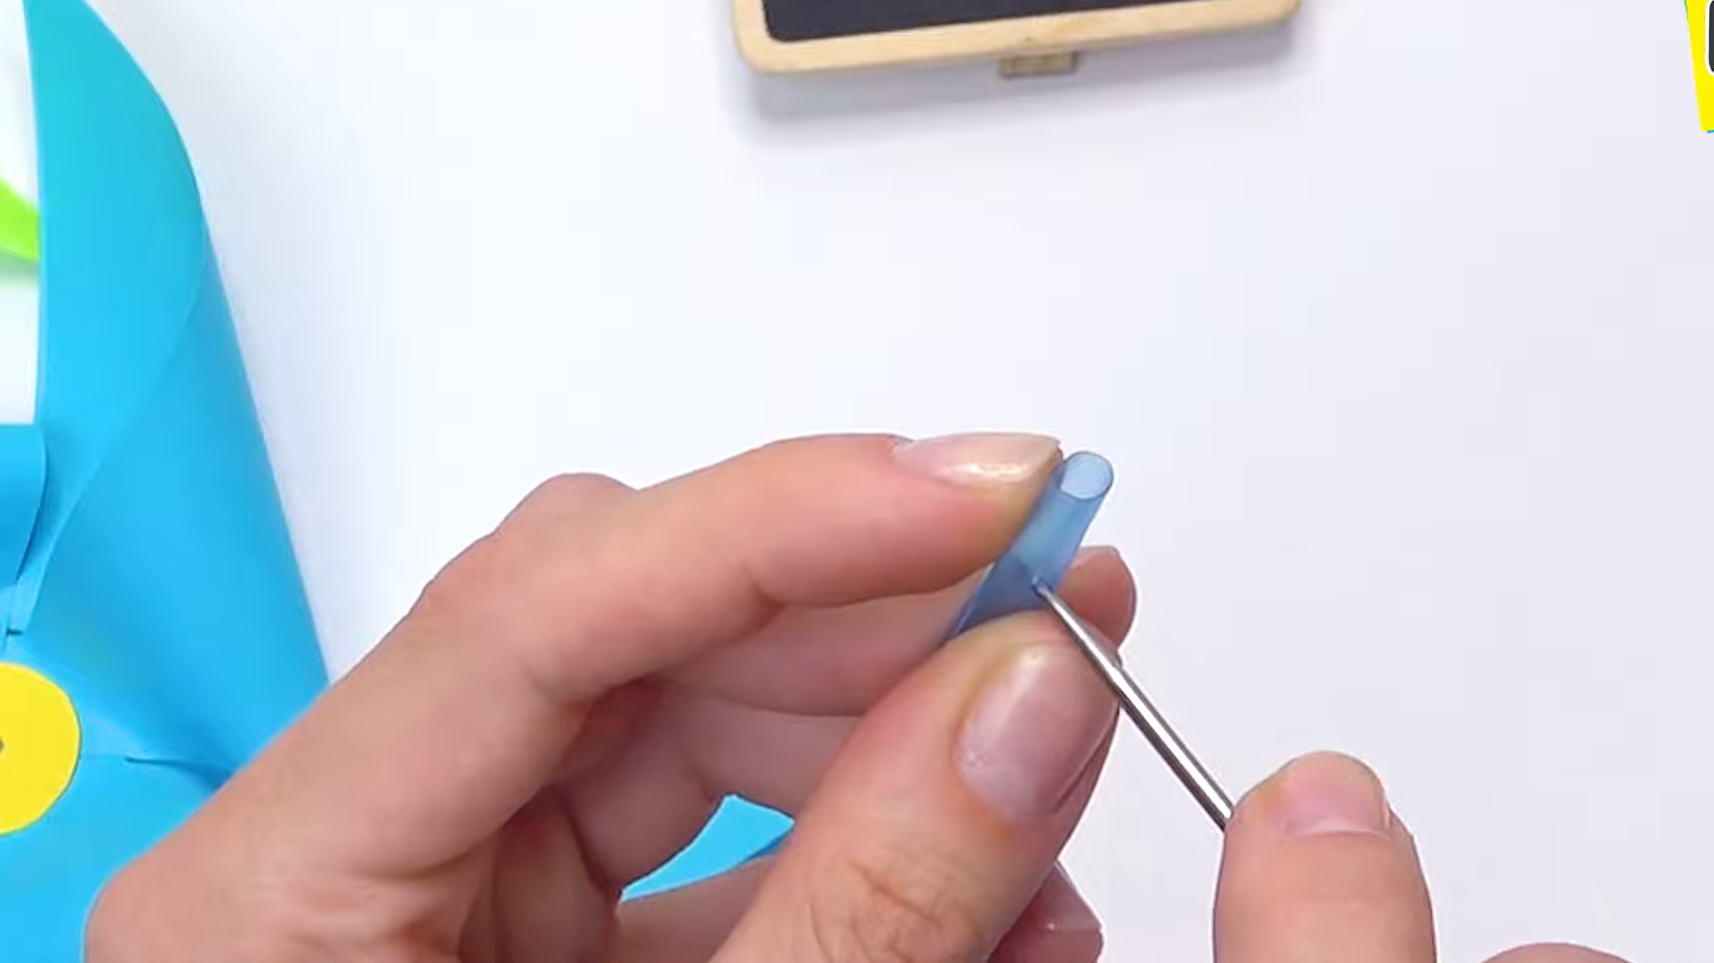
\includegraphics[width= 0.75\linewidth]{8}
		\vspace*{-10pt}
	\end{figure}
	\columnbreak
	\textit{Bước $9$:} Sử dụng kìm để uốn cong và cắt một đoạn thép như hình minh họa.
	\begin{figure}[H]
		\vspace*{-5pt}
		\centering
		\captionsetup{labelformat= empty, justification=centering}
		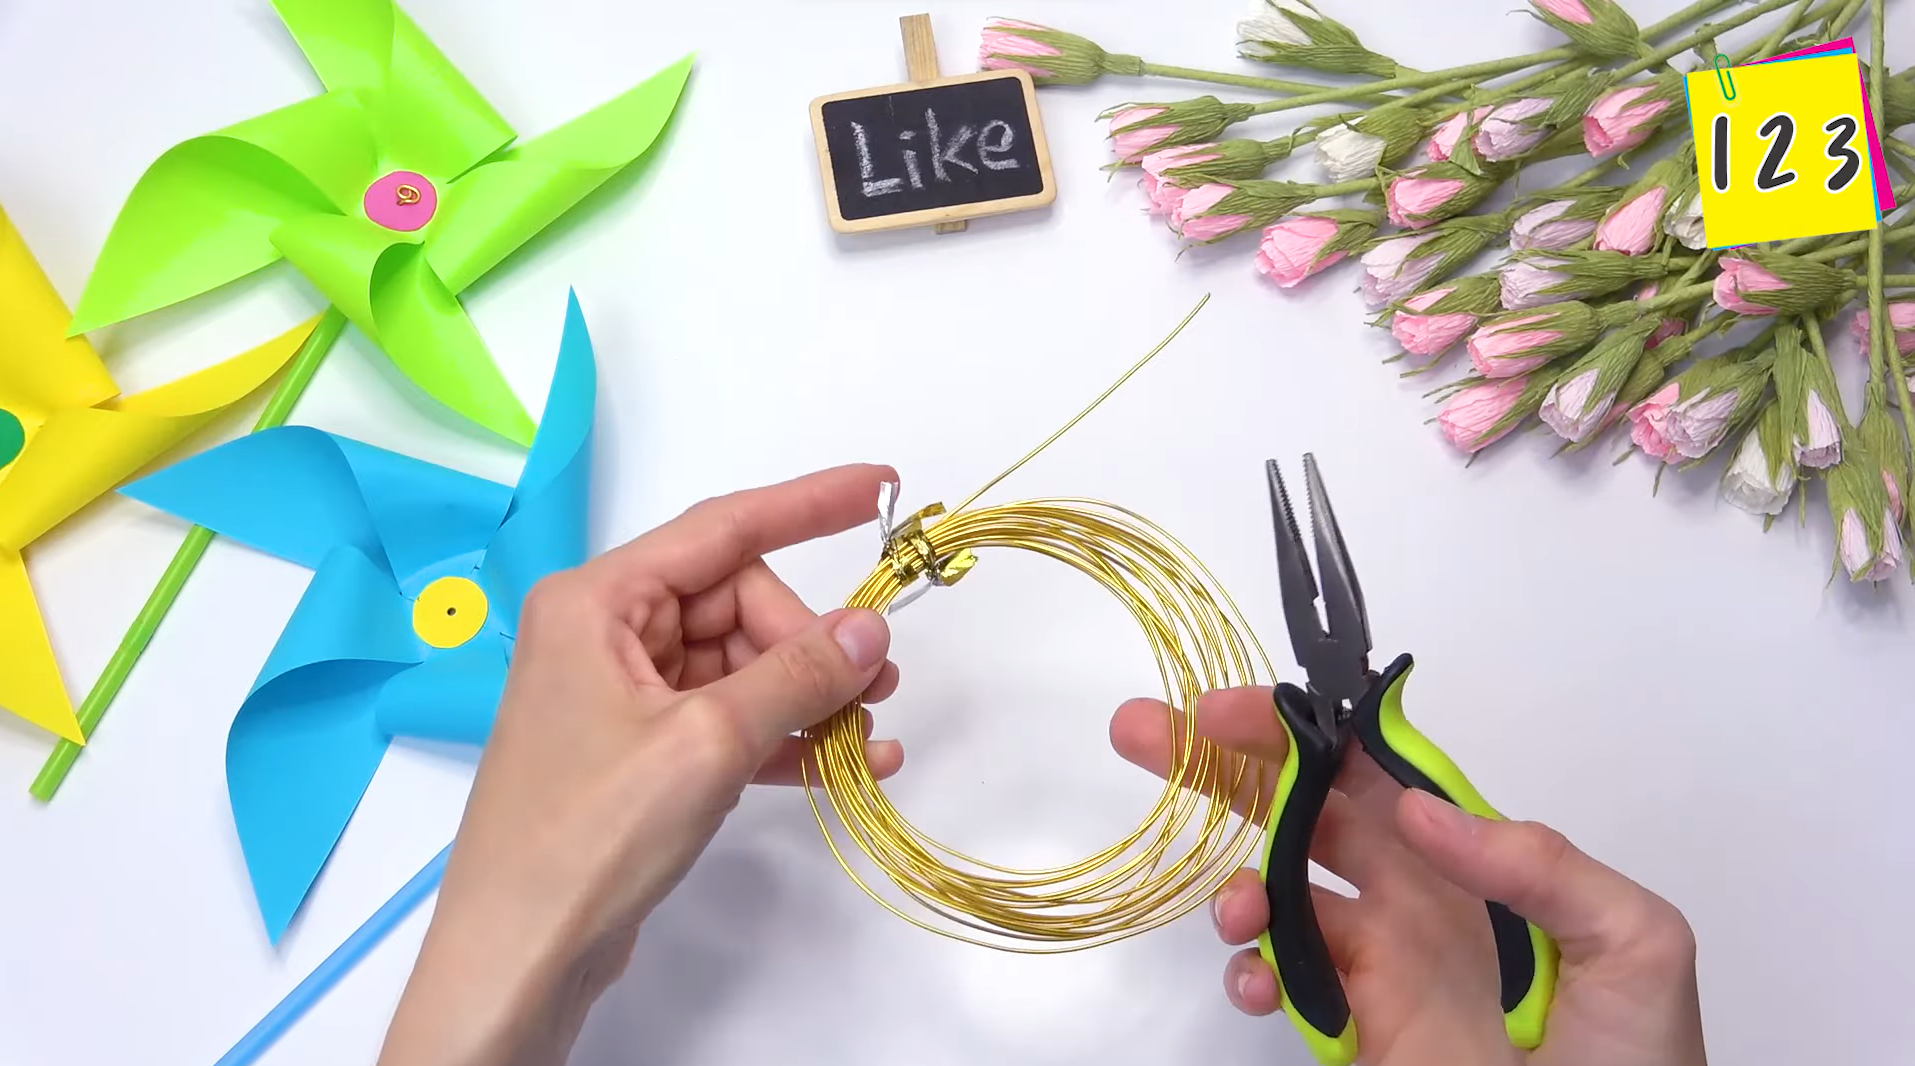
\includegraphics[width= 0.75\linewidth]{9a}
		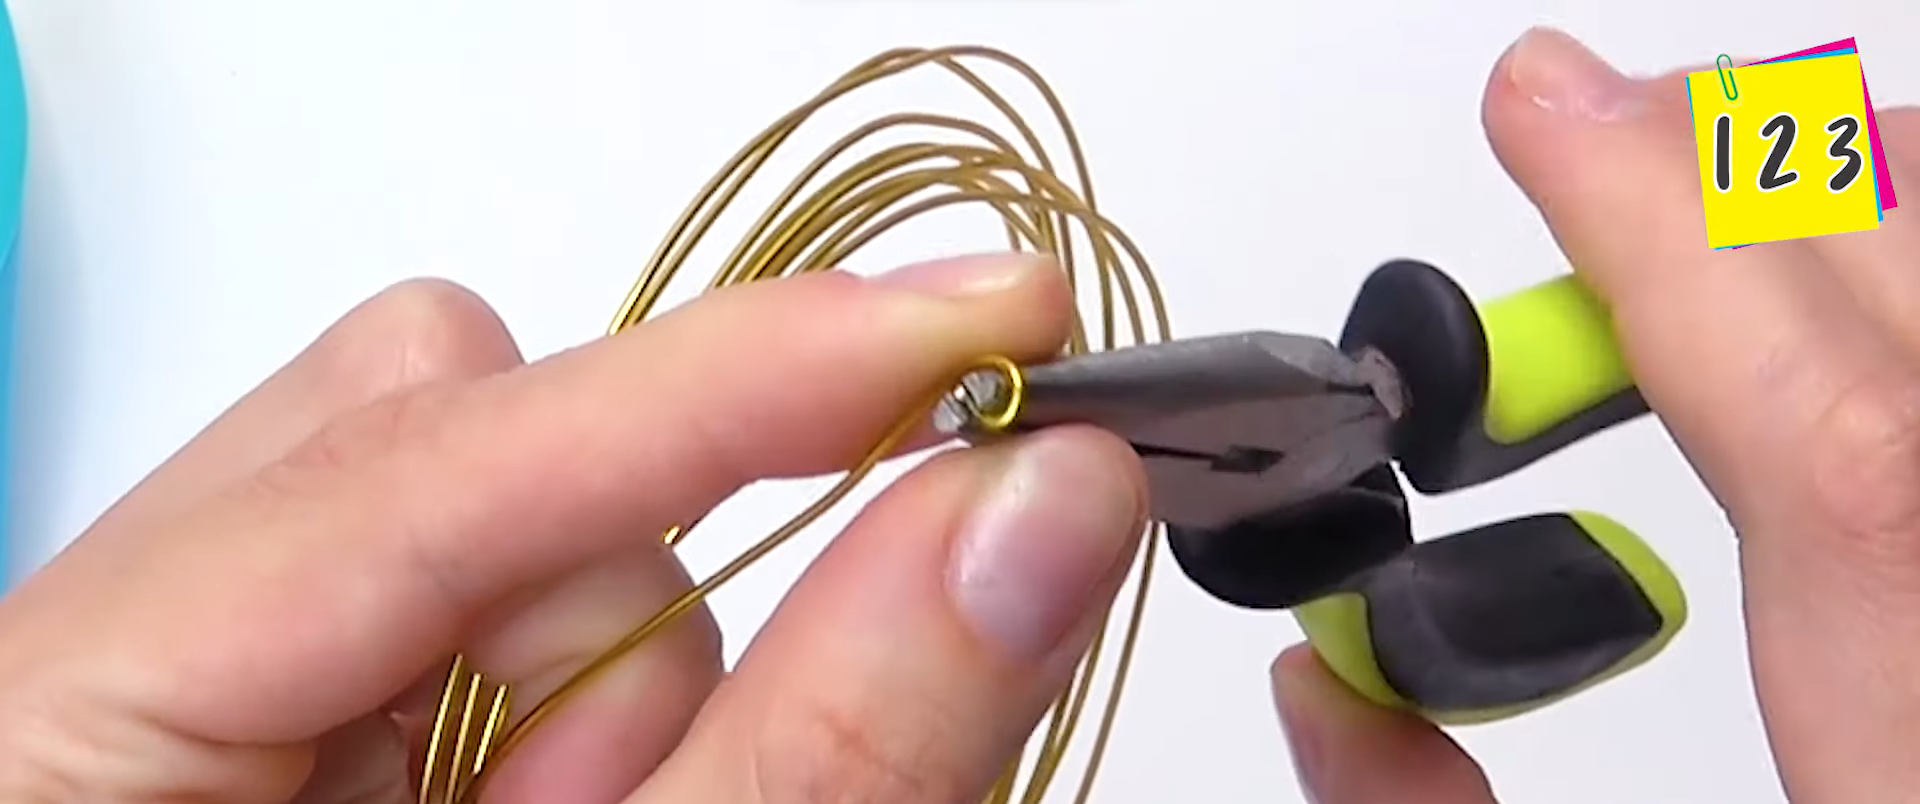
\includegraphics[width= 0.75\linewidth]{9b}
		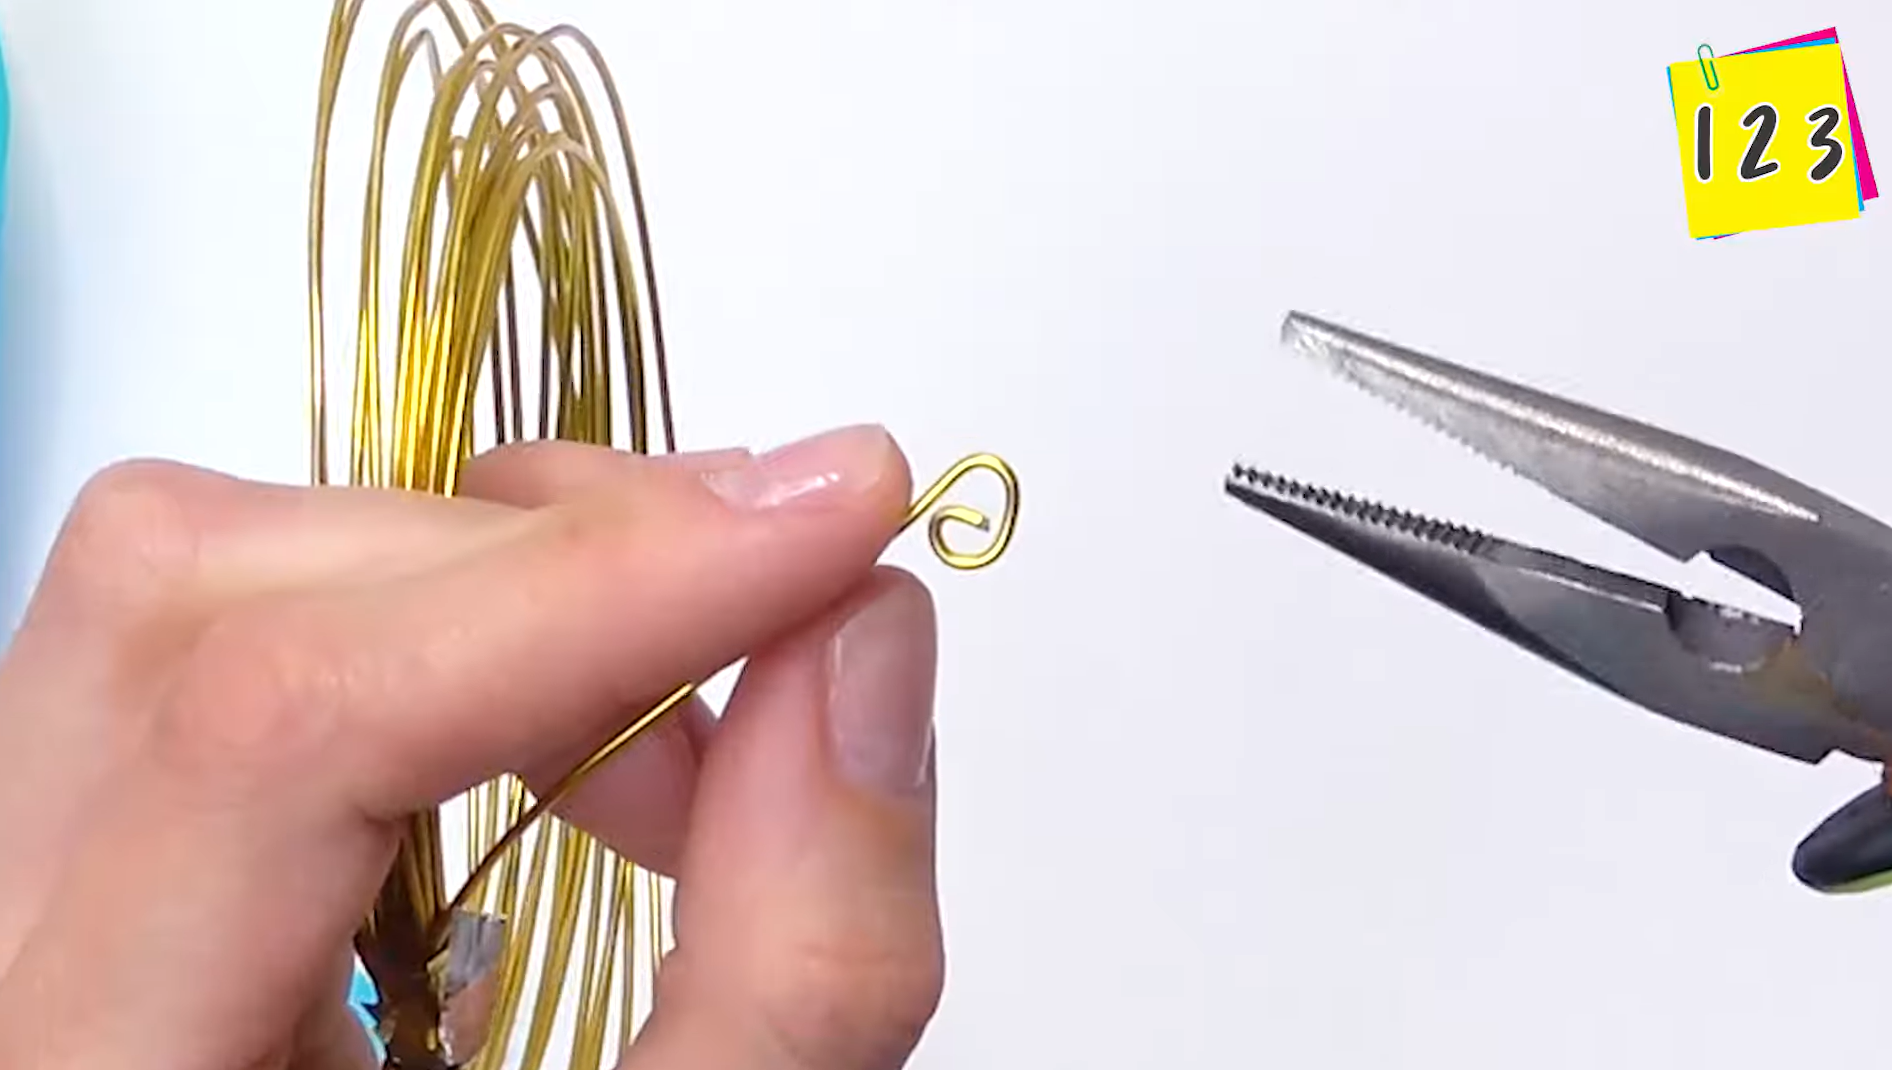
\includegraphics[width= 0.75\linewidth]{9c}
		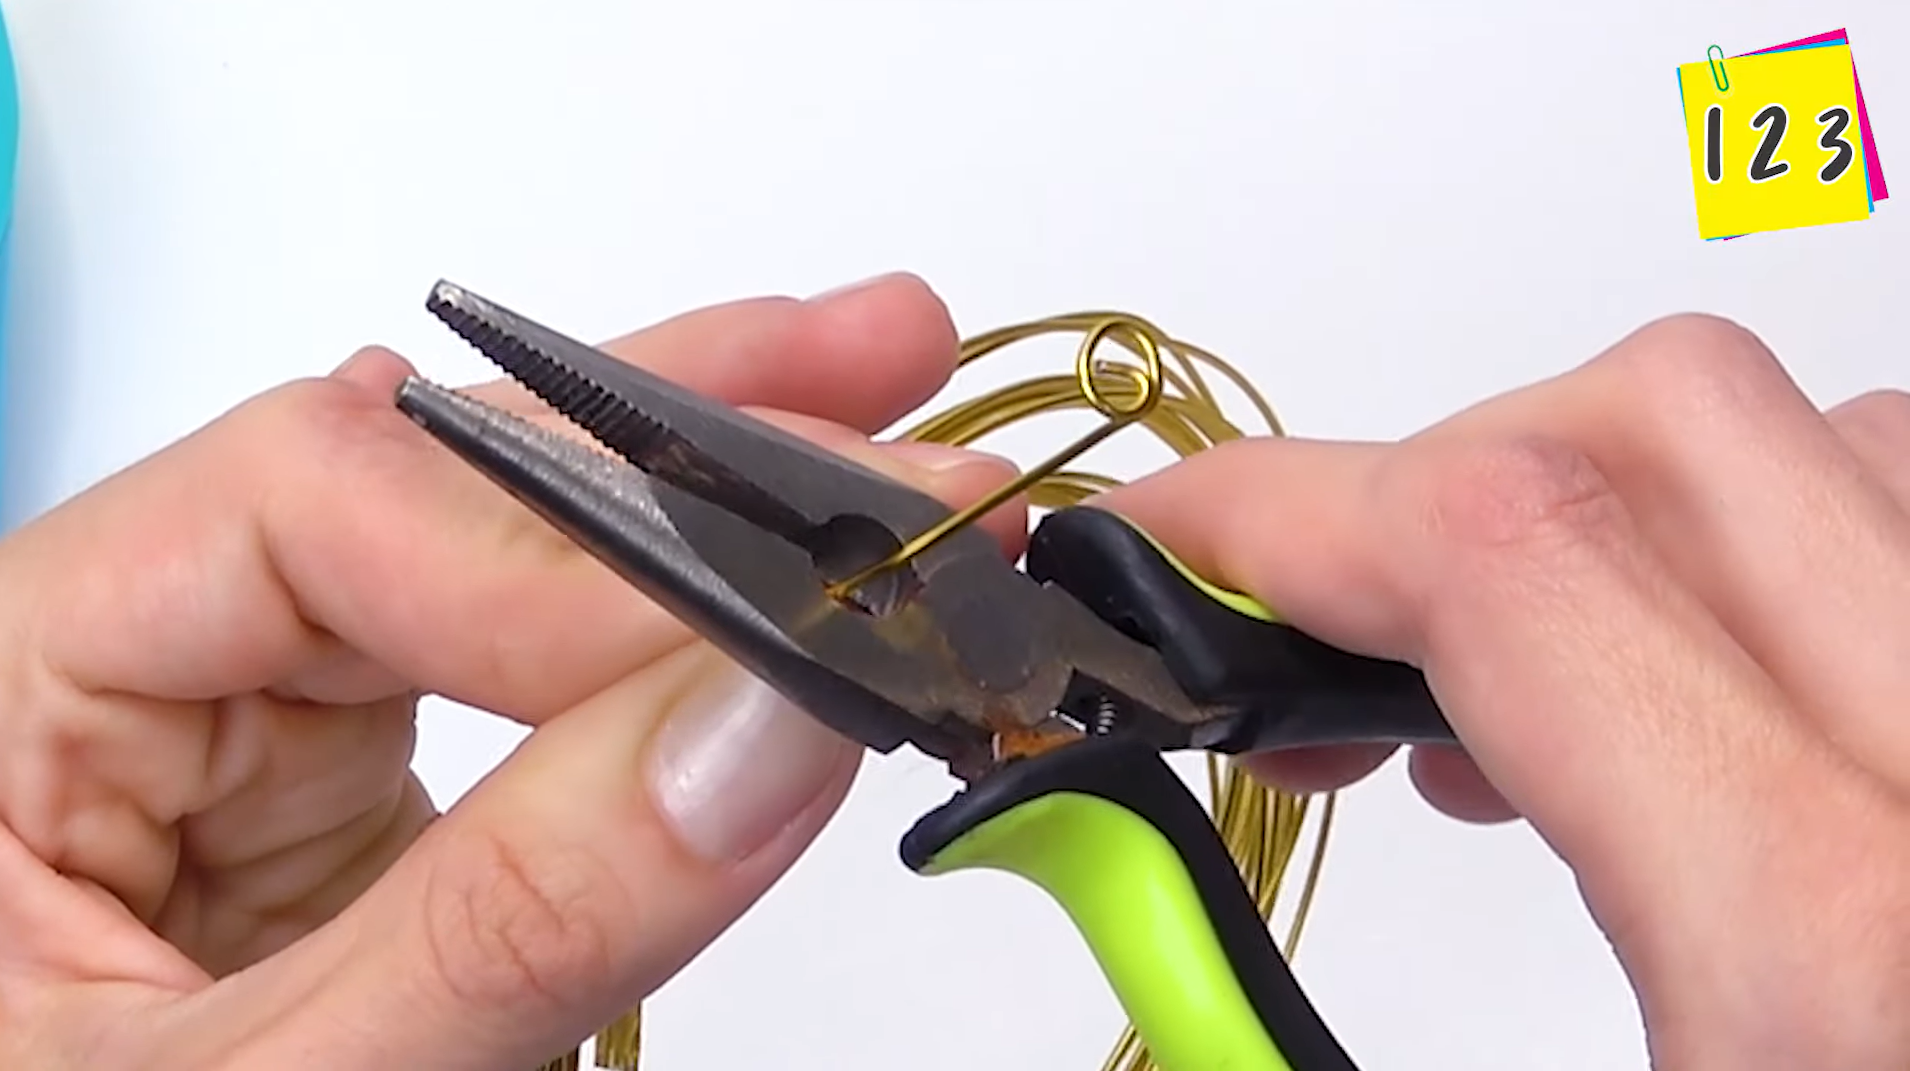
\includegraphics[width= 0.75\linewidth]{9d}
		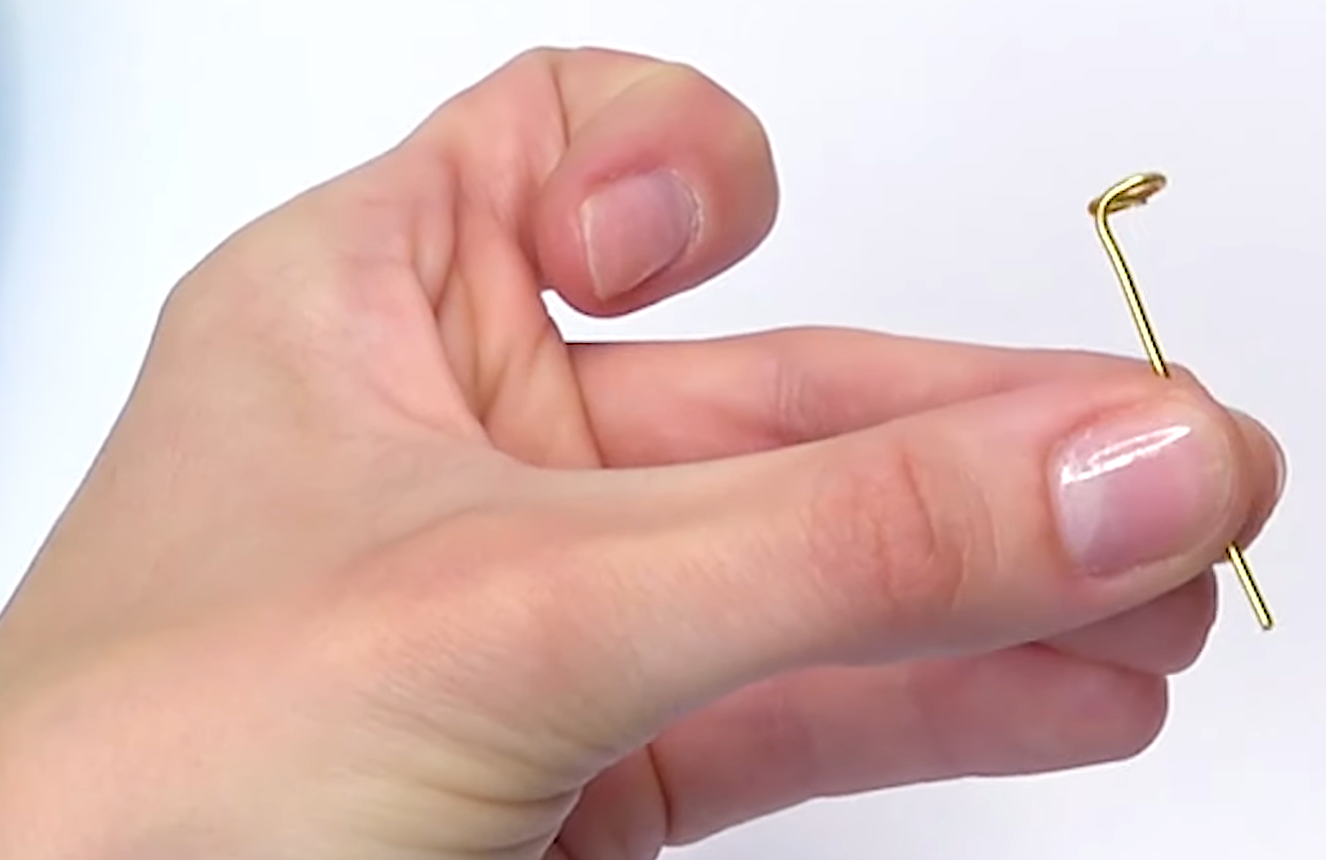
\includegraphics[width= 0.75\linewidth]{9e}
		\vspace*{-10pt}
	\end{figure}
	\textit{Bước $10$:} Sử dụng kìm và đoạn thép này để nối chong chóng với ống hút nhựa.
	\begin{figure}[H]
		\vspace*{5pt}
		\centering
		\captionsetup{labelformat= empty, justification=centering}
		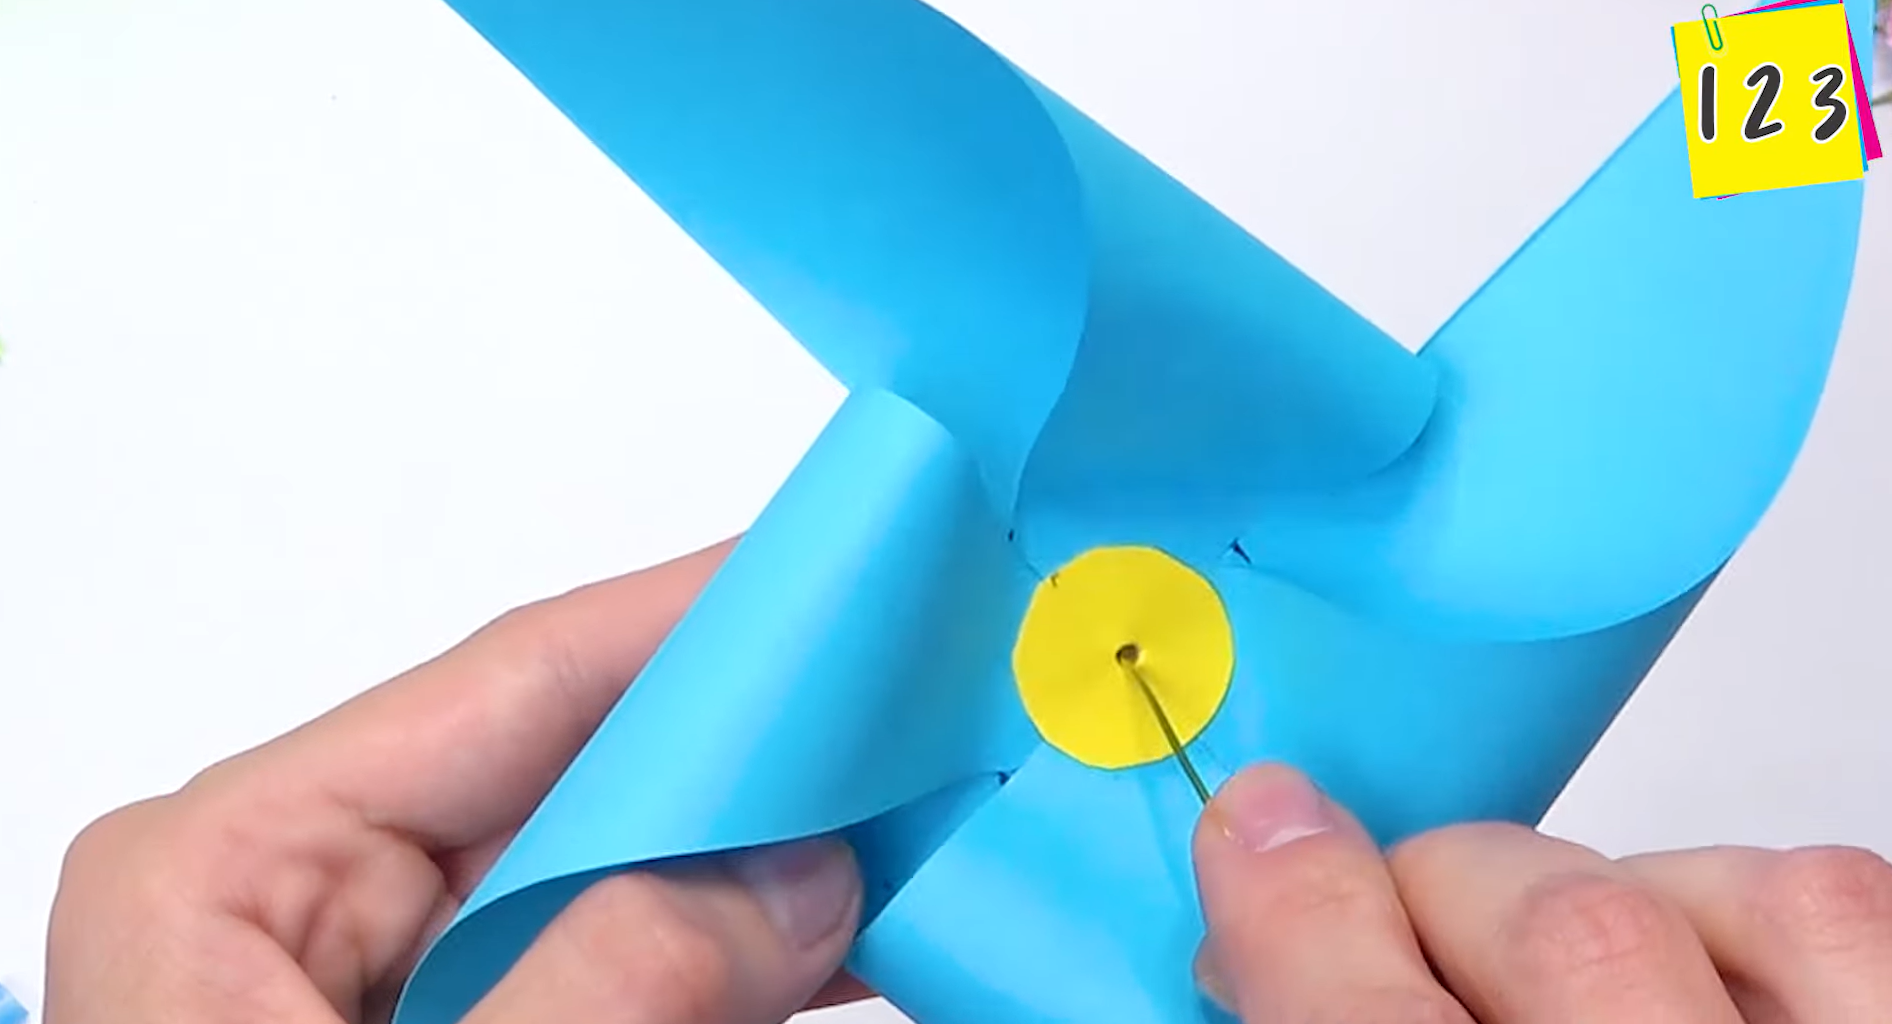
\includegraphics[width= 0.75\linewidth]{10a}
		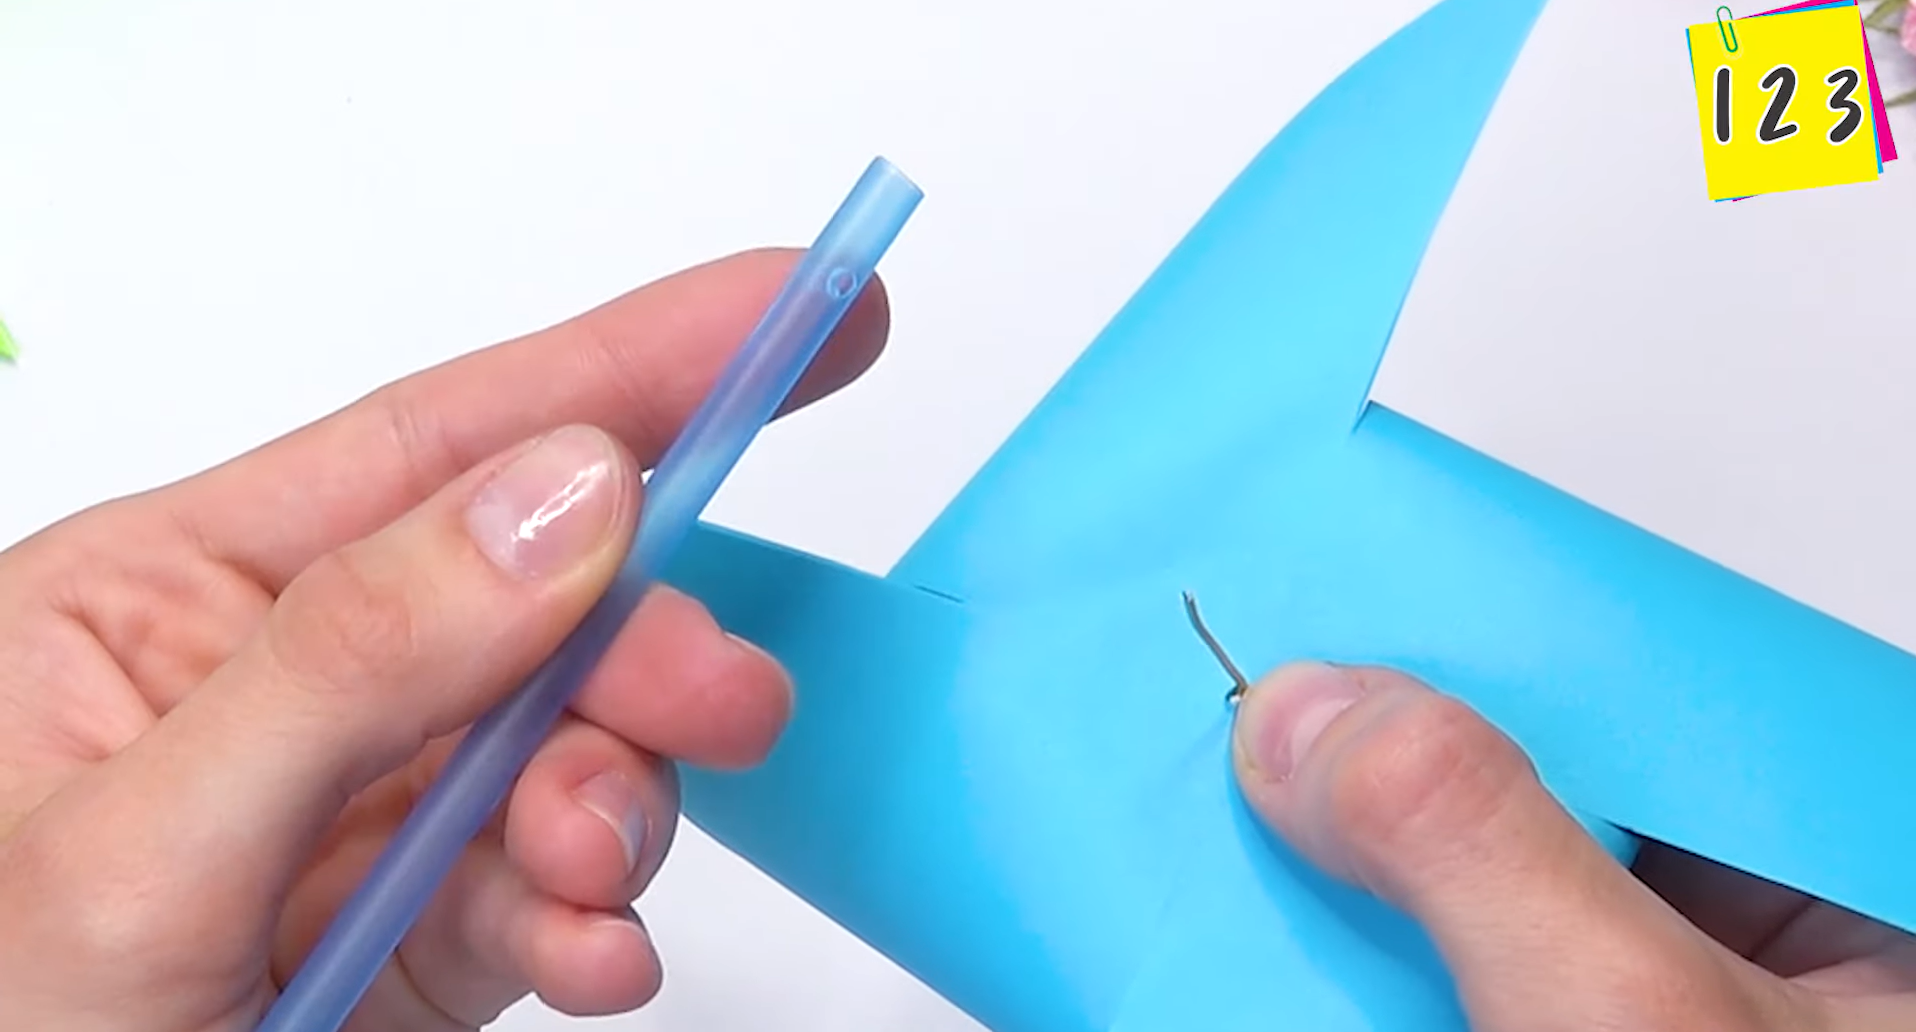
\includegraphics[width= 0.75\linewidth]{10b}
		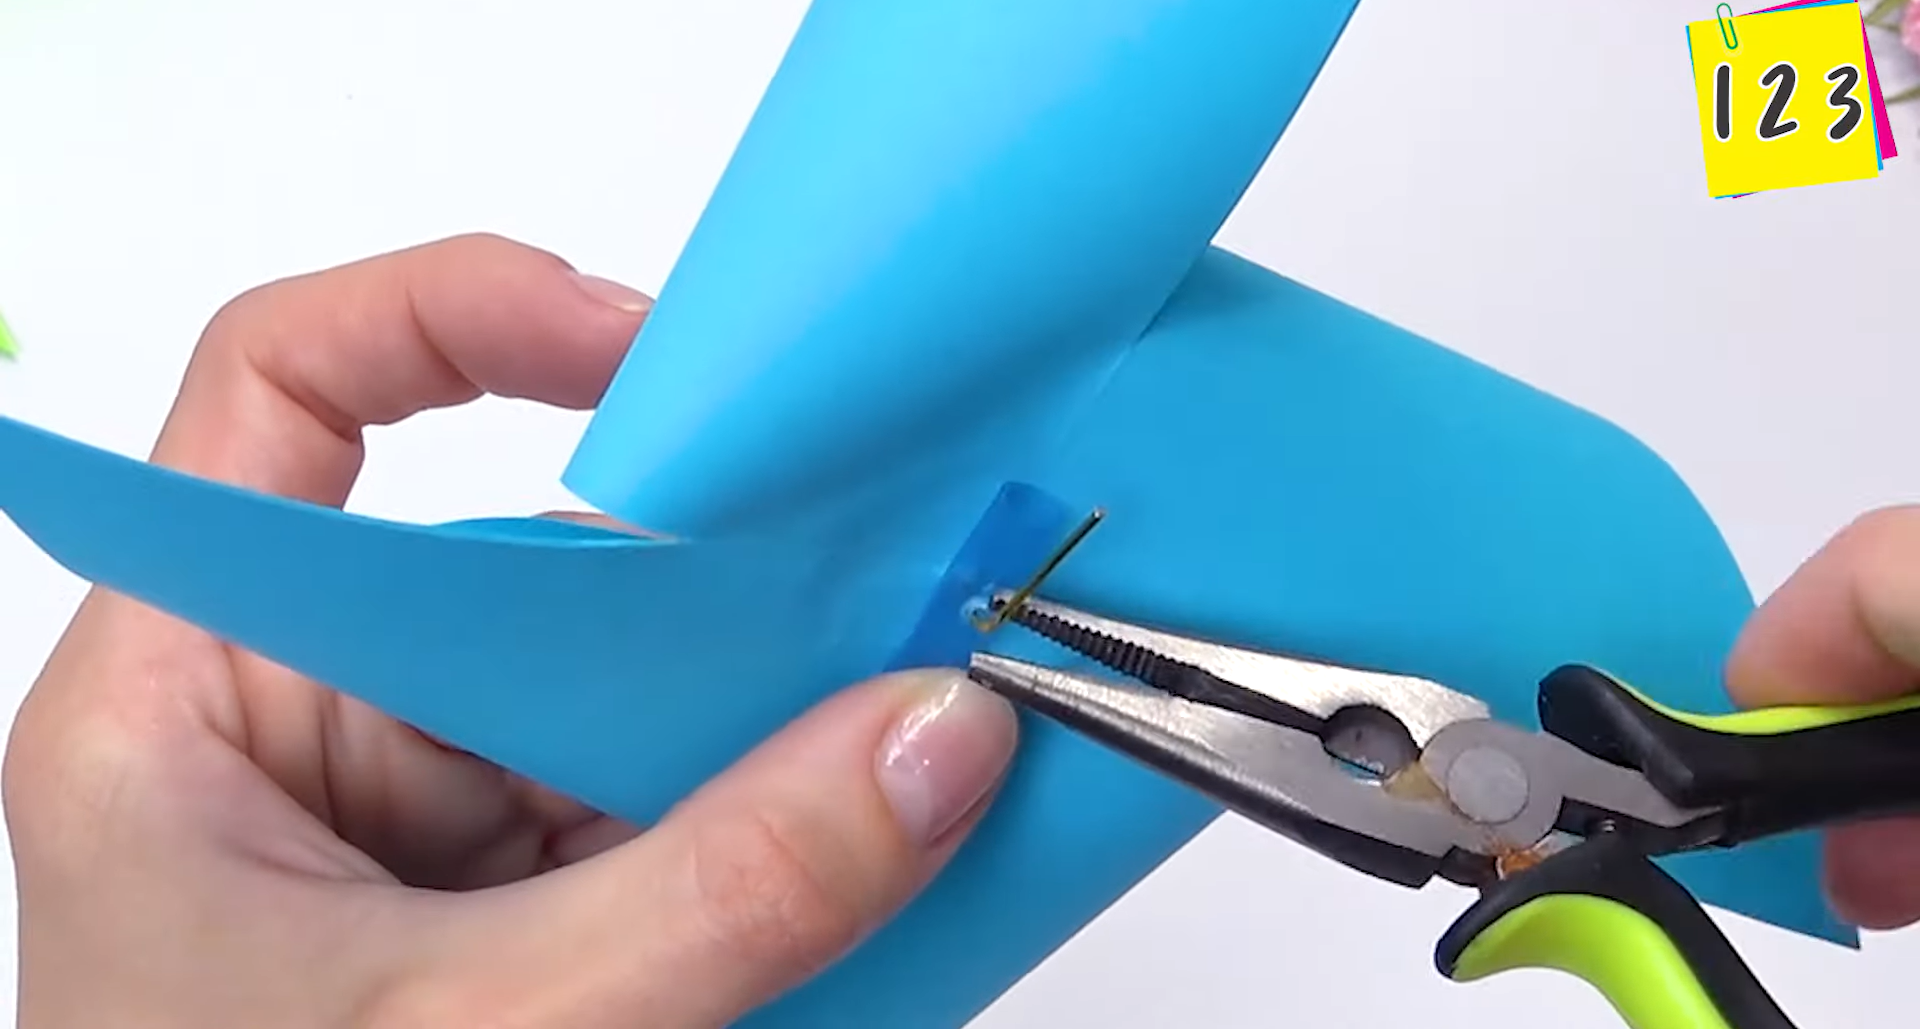
\includegraphics[width= 0.75\linewidth]{10c}
		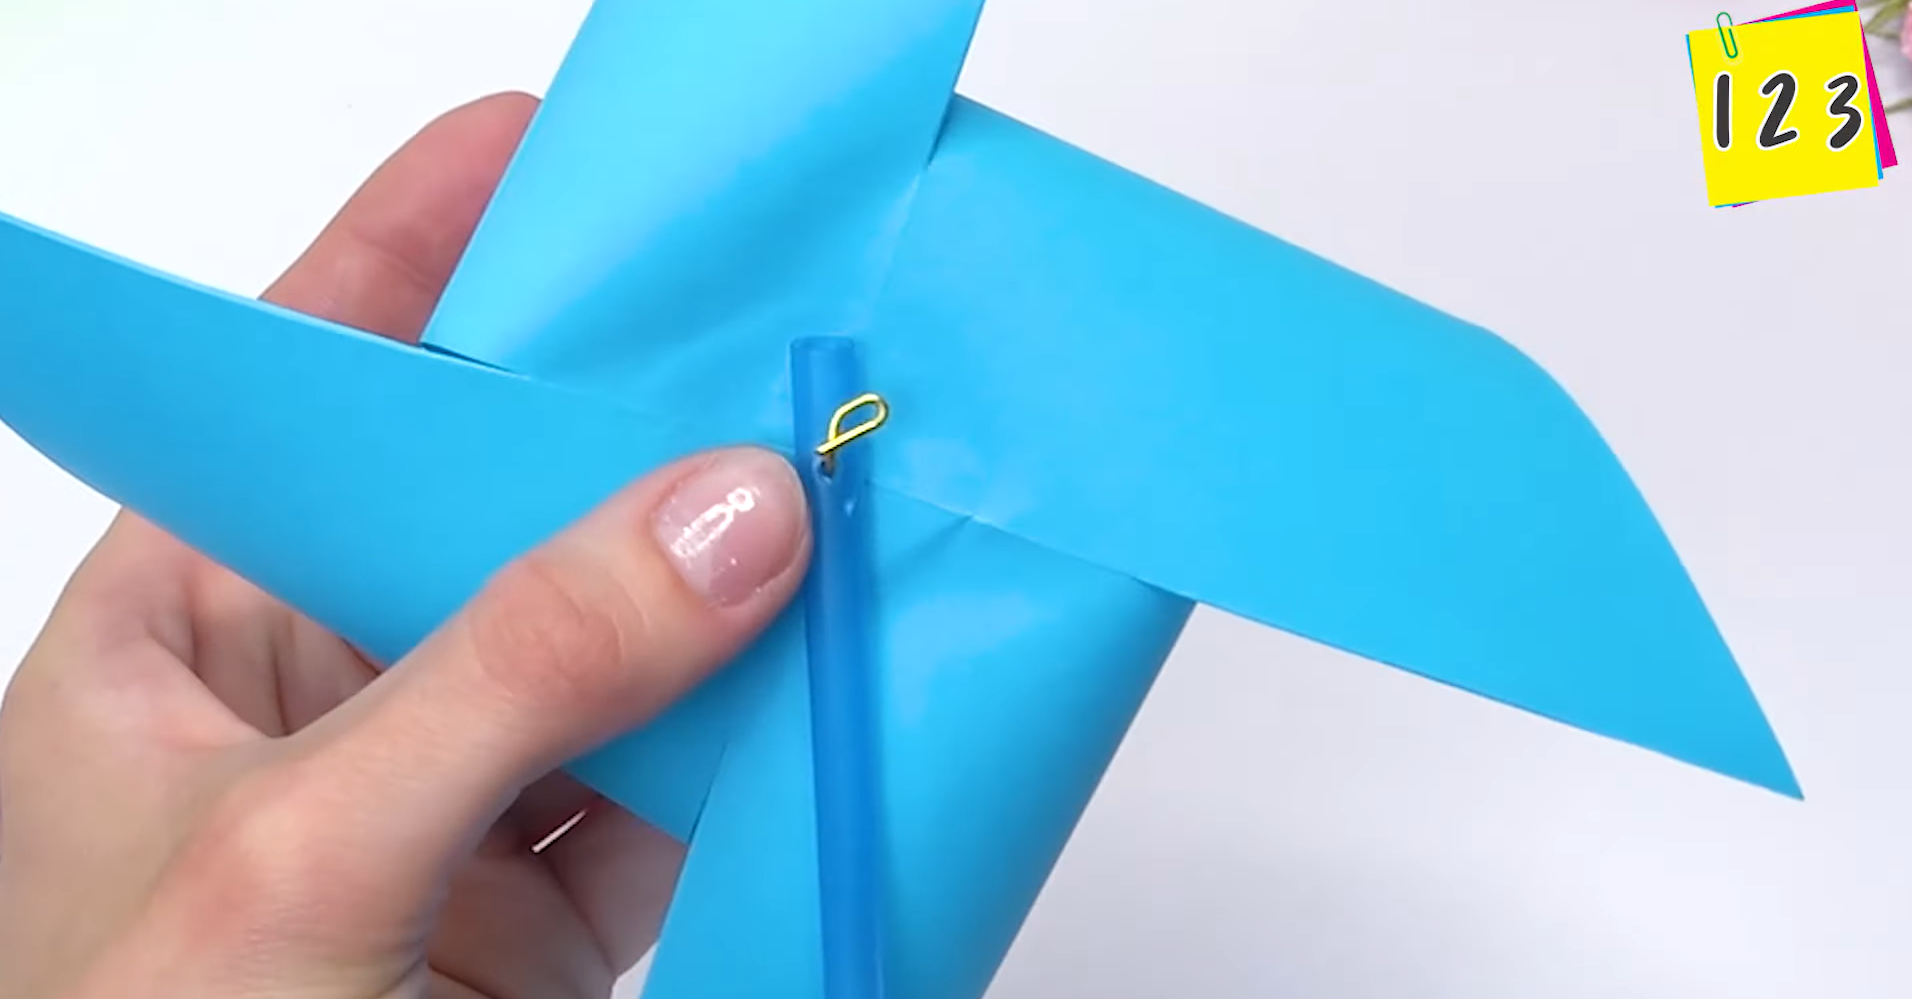
\includegraphics[width= 0.75\linewidth]{10d}
		\vspace*{-10pt}
	\end{figure}
	Vậy là các em đã làm xong chong chóng bốn cánh bằng giấy màu rồi!
	\begin{figure}[H]
		\vspace*{-5pt}
		\centering
		\captionsetup{labelformat= empty, justification=centering}
		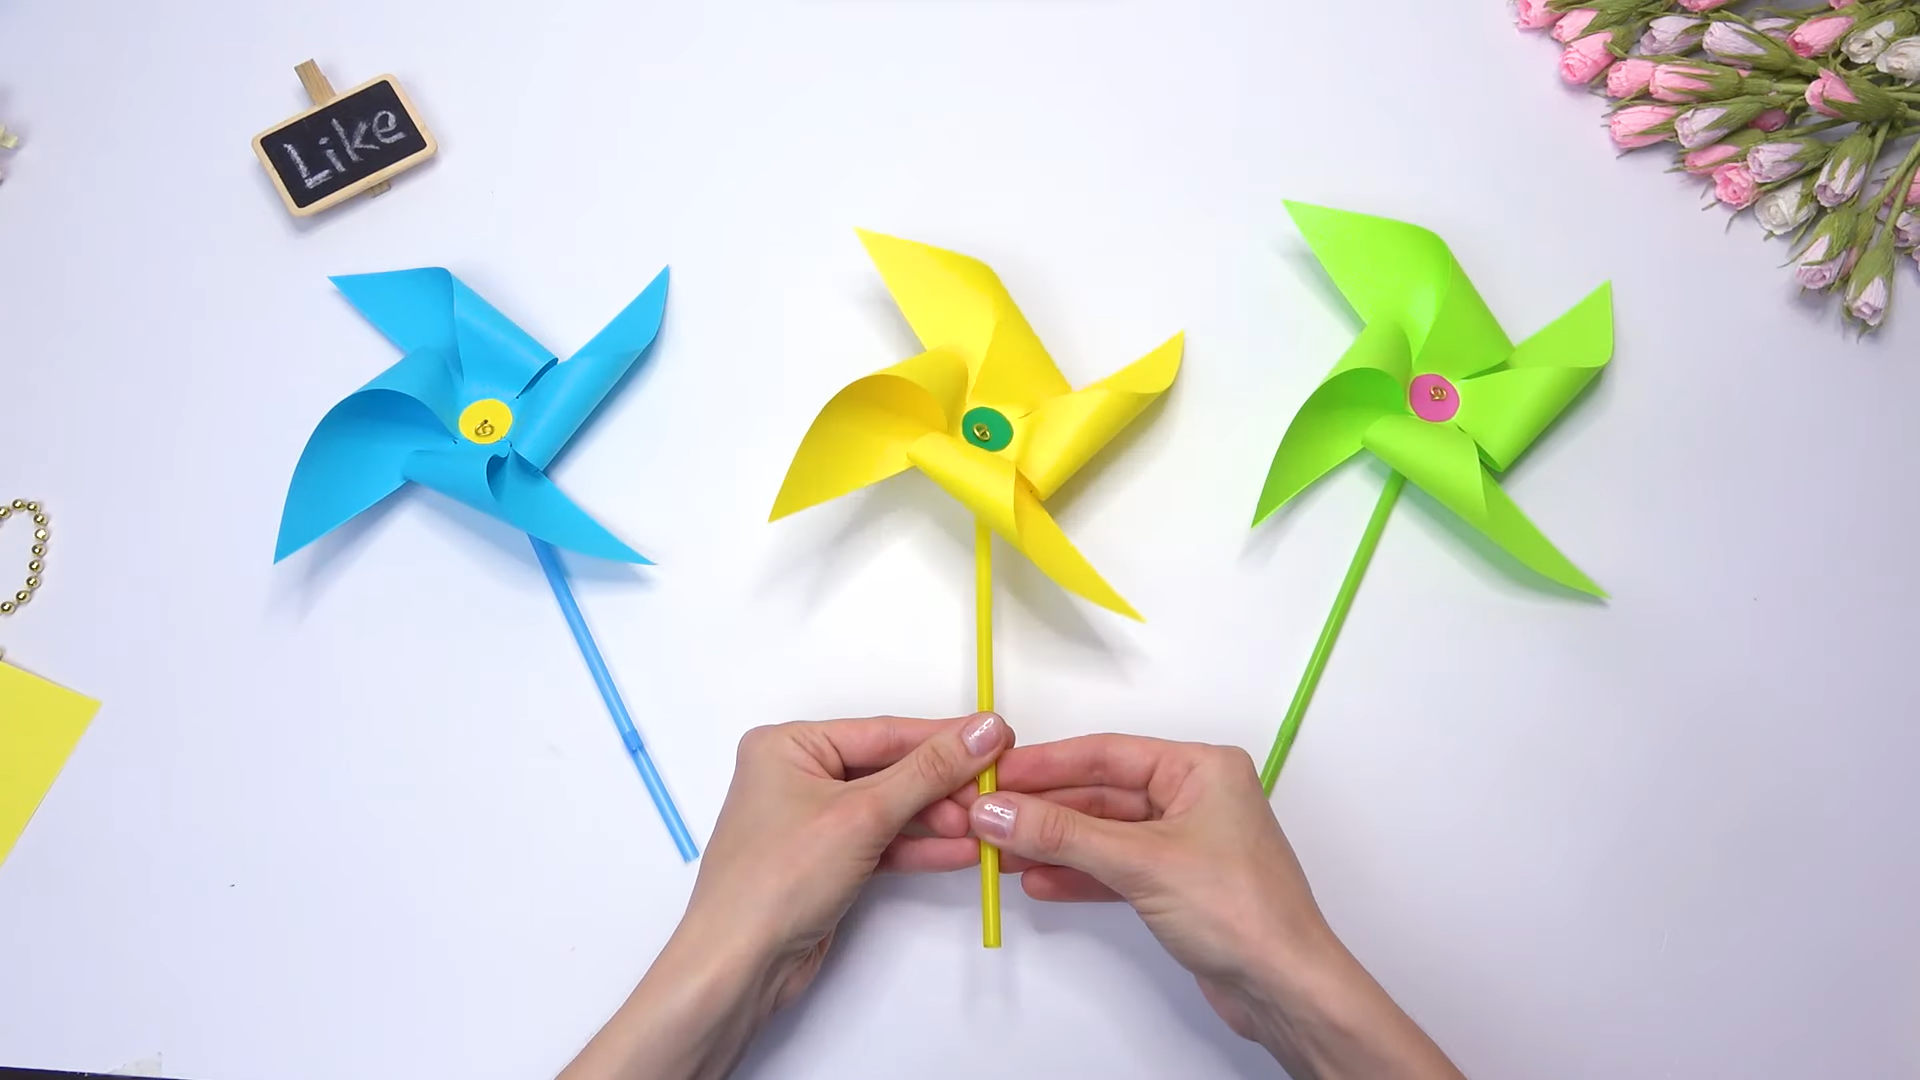
\includegraphics[width= 0.75\linewidth]{11}
		\vspace*{-10pt}
	\end{figure}
	\textbf{\color{toancuabi}Tài liệu tham khảo}
	\vskip 0.1cm
	\url{https://www.youtube.com/watch?v=T8_83cHOYjI&ab_channel=123EasyPaperCraft}\\
	\url{sDIY}
\end{multicols}
\newpage
\graphicspath{{../toancuabi/pic/}}
\begingroup
\AddToShipoutPicture*{\put(149,675){
\includegraphics[scale=1]{../tieude.pdf}}}  
\centering
\endgroup
\vspace*{30pt} 
\begin{multicols}{2}
	Vừa đặt chân tới một hòn đảo, thám tử Xuân Phong đã cho mời $10$ người thổ dân đến gặp mình để điều tra một vụ án từng xảy ra đã hơn nửa thế kỷ trước tại chính hòn đảo xinh đẹp này, tuy nhiên vẫn chưa lần ra manh mối. Người phiên dịch thông báo trước cho thám tử rằng, trong số $10$ người này có một số người đến từ bộ tộc Trung Thực, họ luôn nói thật, còn những người còn lại là từ bộ tộc Lừa Dối, tức họ luôn nói dối. Xuân Phong yêu cầu mỗi người trong số bọn họ nghĩ ra một số nguyên nào đó và sau đó miêu tả về số đó cho thám tử. Mười thổ dân xếp hàng ngang lần lượt trả lời theo thứ tự từ trái qua phải. Người thứ nhất nói: ``Số của tôi lớn hơn $1$", người thứ hai nói: ``Số của tôi lớn hơn $2$", ..., người thứ mười nói: ``Số của tôi lớn hơn $10$". Sau đó một cuộc cãi vã xảy ra, nên các thổ dân quyết định đứng xếp lại theo hàng ngang theo một thứ tự khác, và từ trái qua phải họ lại lần lượt đưa ra các câu trả lời như sau: ``Số của tôi nhỏ hơn $1$", ``Số của tôi nhỏ hơn $2$", ``Số của tôi nhỏ hơn $3$",..., ``Số của tôi nhỏ hơn $10$" (mỗi người nói đúng một câu trong số $10$ câu trên).
	\begin{figure}[H]
		\centering
		\vspace*{-5pt}
		\captionsetup{labelformat= empty, justification=centering}
		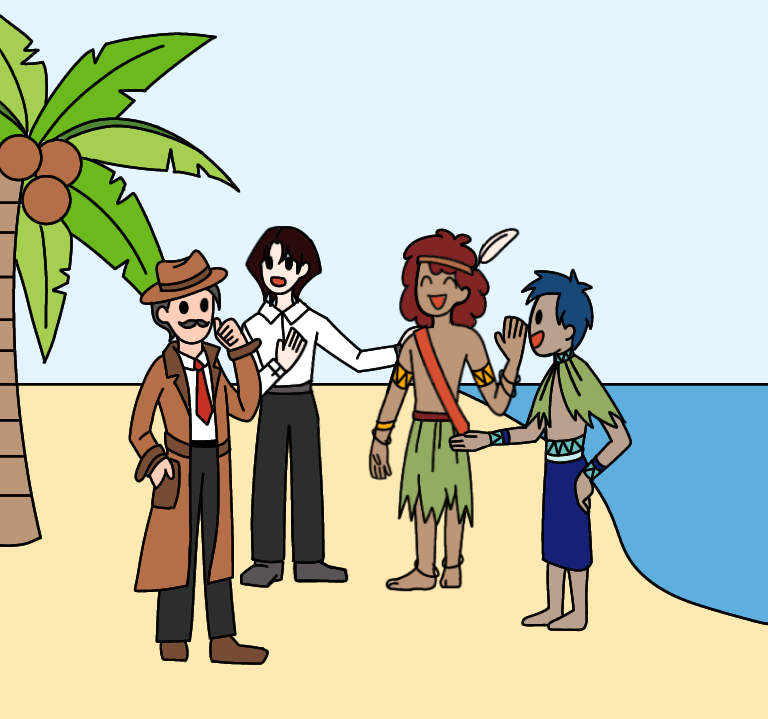
\includegraphics[width=1\linewidth]{xuanphong}
		\vspace*{-15pt}
	\end{figure}
	Các em có thể giúp Xuân Phong xác định xem trong số $10$ thổ dân kỳ lạ trên có nhiều nhất bao nhiêu người đến từ bộ tộc Trung Thực được hay không?
%	Lời giải
%	
%	Ta sẽ chứng minh rằng không có ai đến từ bộ tộc Trung Thực (gọi tắt là người Trung Thực) nói một trong các câu ``Số của tôi lớn hơn 9" hoặc ``Số của tôi lớn hơn 10". Thật vậy, nếu điều đó xảy ra thì số mà người Trung Thực đó nghĩ ra không thể nhỏ hơn 10. Nhưng khi đó, anh ta không thể nói bất kỳ một trong các câu: ``Số của tôi nhỏ hơn 1", ``Số của tôi nhỏ hơn 2",…, ``Số của tôi nhỏ hơn 10". Vì vậy, số các người Trung Thực không thể lớn hơn 8 (người).
%	
%	Ta sẽ chỉ ra có thể xảy ra trường hợp có đúng 8 người Trung Thực. Giả sử lúc đầu có 8 người Trung Thực đứng đầu tiên từ trái qua phải: người Trung Thực thứ nhất nghĩ ra số 2, người thứ hai nghĩ ra số 3,… người thứ tám nghĩ ra số 9, còn hai người Lừa Dối ở cuối hàng nghĩ ra số 5 và số 6. 
%	
%	Khi đó người Trung Thực thứ k có thể nói các câu: ``Số của tôi lớn hơn k" và ``Số của tôi nhỏ hơn k+2"; còn một người Lừa Dối có thể nói các câu: ``Số của tôi lớn hơn 9" và ``Số của tôi nhỏ hơn 1", người Lừa Dối còn lại có thể nói các câu: ``Số của tôi lớn hớn 10" và ``Số của tôi nhỏ hơn 2". 
%	
%	Đáp số: Có tối đa 8 người đến từ bộ tộc Trung Thực.
\end{multicols}
\vspace*{-10pt}
{\color{toancuabi}\rule{1\linewidth}{0.1pt}}
\begingroup
\AddToShipoutPicture*{\put(120,265){
\includegraphics[scale=1]{../tieude11.pdf}}} 
\centering
\endgroup
\vspace*{48pt}

\begin{multicols}{2}
	$\pmb{1.}$ 	Cô giáo phát cho $4$ em học sinh Mai, Tuấn, Vinh, Ngọc tổng cộng $66$ chiếc bút. 	Mai được phát nhiều hơn Tuấn một chiếc
	\begin{figure}[H]
		\centering
		\vspace*{-5pt}
		\captionsetup{labelformat= empty, justification=centering}
		
\includegraphics[width=0.75\linewidth]{b1}
		\vspace*{-5pt}
	\end{figure}
  bút, Vinh được phát nhiều hơn Mai một chiếc bút, còn Ngọc lại được phát nhiều hơn Vinh một chiếc bút. Hỏi Ngọc được cô giáo phát cho bao nhiêu chiếc bút?
\vskip 0.1cm
	$\pmb{2.}$ 	Ba người bạn cùng vào quán ăn sáng. Một người gọi mua $4$ chiếc bánh ngọt, một cốc sữa và $10$ chiếc quẩy và trả hết $40000$ đồng. Người thứ hai gọi mua $3$ chiếc bánh ngọt, một cốc sữa và $7$ chiếc quẩy và trả hết $30000$ đồng. Người thứ ba phải trả bao nhiêu tiền nếu anh ta chỉ mua một chiếc bánh ngọt, một cốc sữa và một chiếc quẩy?
	\begin{figure}[H]
			\centering
			\vspace*{-5pt}
			\captionsetup{labelformat= empty, justification=centering}
			
\includegraphics[width=0.85\linewidth]{b2}
			\vspace*{-5pt}
		\end{figure}
	$\pmb{3.}$ 	Tất cả các quân của bộ domino (gồm $28$ quân) được xếp đúng thành một dãy xích theo quy luật của trò chơi: điểm số tại một đầu của quân cờ này trùng với điểm số tại một đầu của quân cờ kia. Một đầu của dãy xích có $5$ điểm. Hỏi đầu kia của dãy có bao nhiêu điểm?
	\begin{figure}[H]
			\centering
			\vspace*{-5pt}
			\captionsetup{labelformat= empty, justification=centering}
			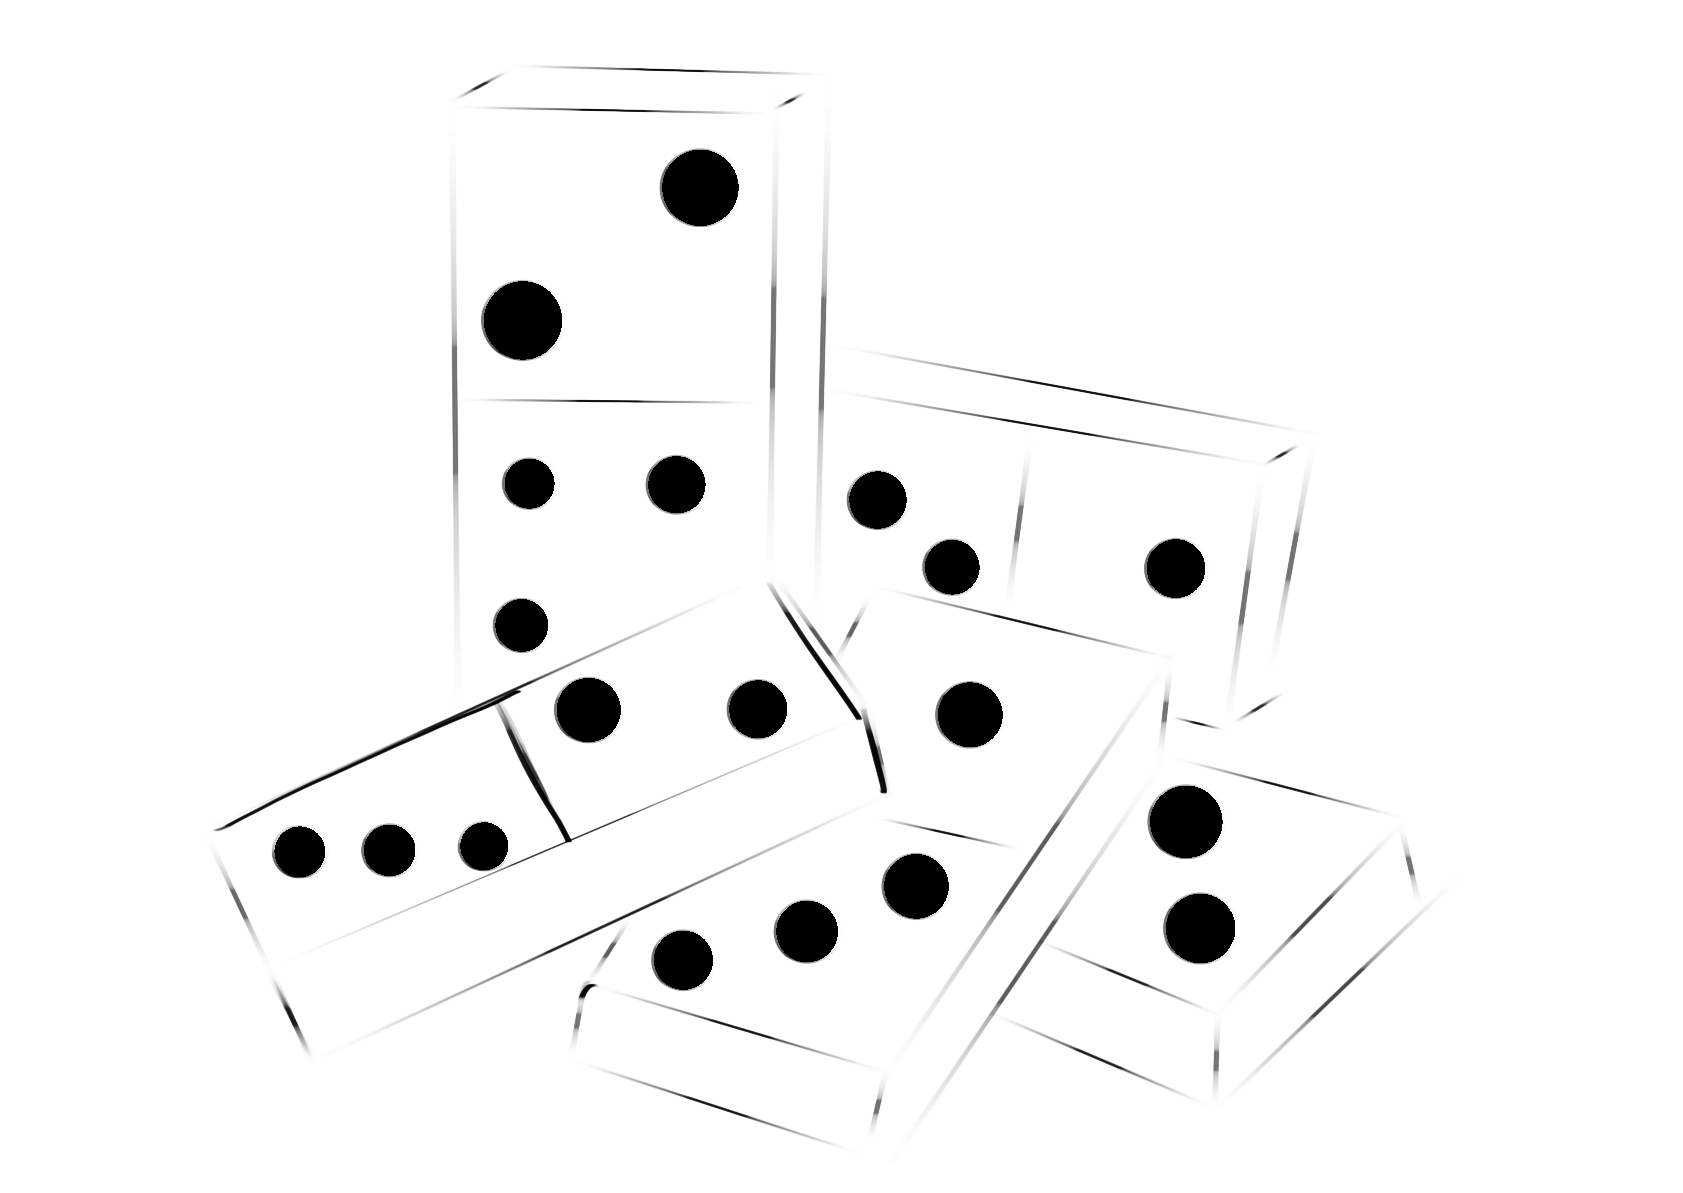
\includegraphics[width=0.9\linewidth]{b3}
			\vspace*{-20pt}
	\end{figure}
	$\pmb{4.}$ Ở vùng Rừng Núi nọ, chỉ có các giống người Thần Tiên và người Lùn sinh sống. Người Lùn luôn nói dối nếu nói về số vàng của mình, còn luôn nói thật trong tất cả các trường hợp còn lại. Người Thần Tiên thì luôn nói dối khi nói về người Lùn, còn luôn nói thật trong các trường hợp còn lại. Một lần nọ, hai người dân vùng Rừng Núi nói chuyện với nhau:
	\begin{figure}[H]
		\centering
		\vspace*{-5pt}
		\captionsetup{labelformat= empty, justification=centering}
		
\includegraphics[width=0.9\linewidth]{b4}
		\vspace*{-10pt}
	\end{figure}
	$A.$ \textit{Toàn bộ số vàng mà tôi có là do tôi đã đánh cắp ở chỗ con Rồng.}
	\vskip 0.1cm
	$B.$ \textit{Anh nói dối.}
	\vskip 0.1cm
	Em hãy xác định xem mỗi người trong số hai người đó là người Thần Tiên hay là người Lùn.
	\vskip 0.1cm
	$\pmb{5.}$ 	Ba bạn Vinh, Phúc và Khánh tham gia một cuộc đua xe đạp trong nhà theo đường đua vòng tròn, cùng xuất phát một lúc. Vinh đạp xe mỗi vòng quanh sân nhanh hơn Phúc $2$ giây, còn Phúc đạp xe mỗi vòng quanh sân nhanh hơn Khánh $3$ giây. Khi Vinh về đến đích để kết thúc quãng đua của mình, thì Phúc phải đạp thêm $1$ vòng còn Khánh phải đạp thêm $2$ vòng nữa mới kết thúc. Hỏi quãng đường đua bao gồm mấy vòng quanh sân?
	\begin{figure}[H]
			\centering
			\vspace*{-5pt}
			\captionsetup{labelformat= empty, justification=centering}
			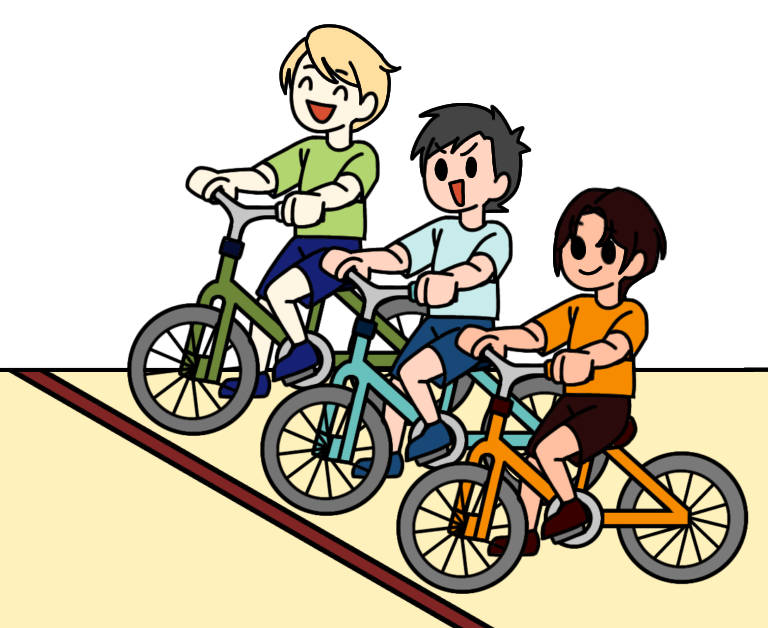
\includegraphics[width=1\linewidth]{b5}
			\vspace*{-20pt}
		\end{figure}
	$\pmb{6.}$ 	Ở một vườn bách thú nọ có rất nhiều chú khỉ, nhưng mỗi chú khỉ sẽ chỉ hạnh phúc nếu được cho ăn ba loại hoa quả khác nhau. Hỏi có nhiều nhất bao nhiêu chú khỉ sẽ hạnh phúc, nếu người chăm sóc vườn thú chỉ có $20$ quả lê, $30$ quả táo, $40$ quả đào và $50$ quả quýt?
	\begin{figure}[H]
			\centering
			\vspace*{-10pt}
			\captionsetup{labelformat= empty, justification=centering}
			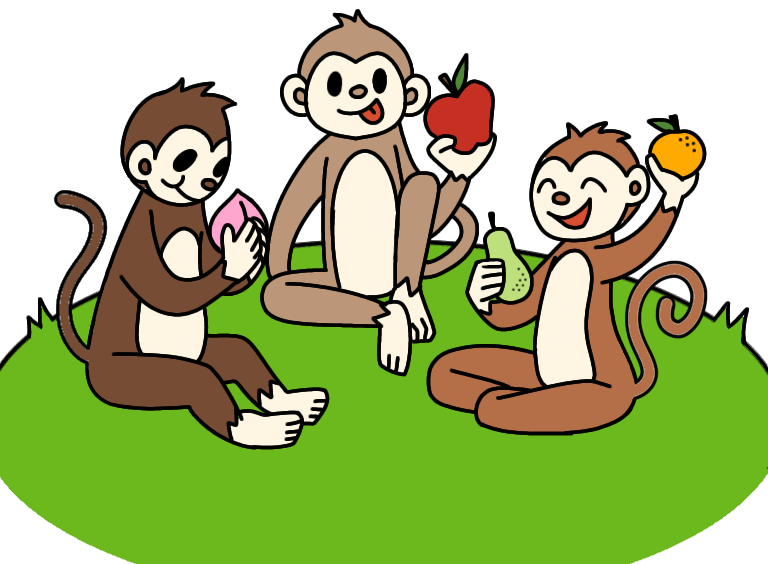
\includegraphics[width=1\linewidth]{b6}
			\vspace*{-5pt}
		\end{figure}
\end{multicols}
\newpage
\begingroup
\AddToShipoutPicture*{\put(116,640){
\includegraphics[scale=1]{../tieude2.pdf}}} 
\centering
\endgroup
\vspace*{65pt}

\begin{multicols}{2}
	$\pmb{1.}$ Nàng Lọ Lem đi lạc vào trong rừng. Theo lời khuyên của bà tiên, nàng tìm thấy ba chiếc rương đựng những hạt dẻ có thể đem lại điều ước. Chiếc rương thứ nhất có ít hơn $6$ hạt dẻ
	\begin{figure}[H]
		\centering
		\vspace*{-5pt}
		\captionsetup{labelformat= empty, justification=centering}
		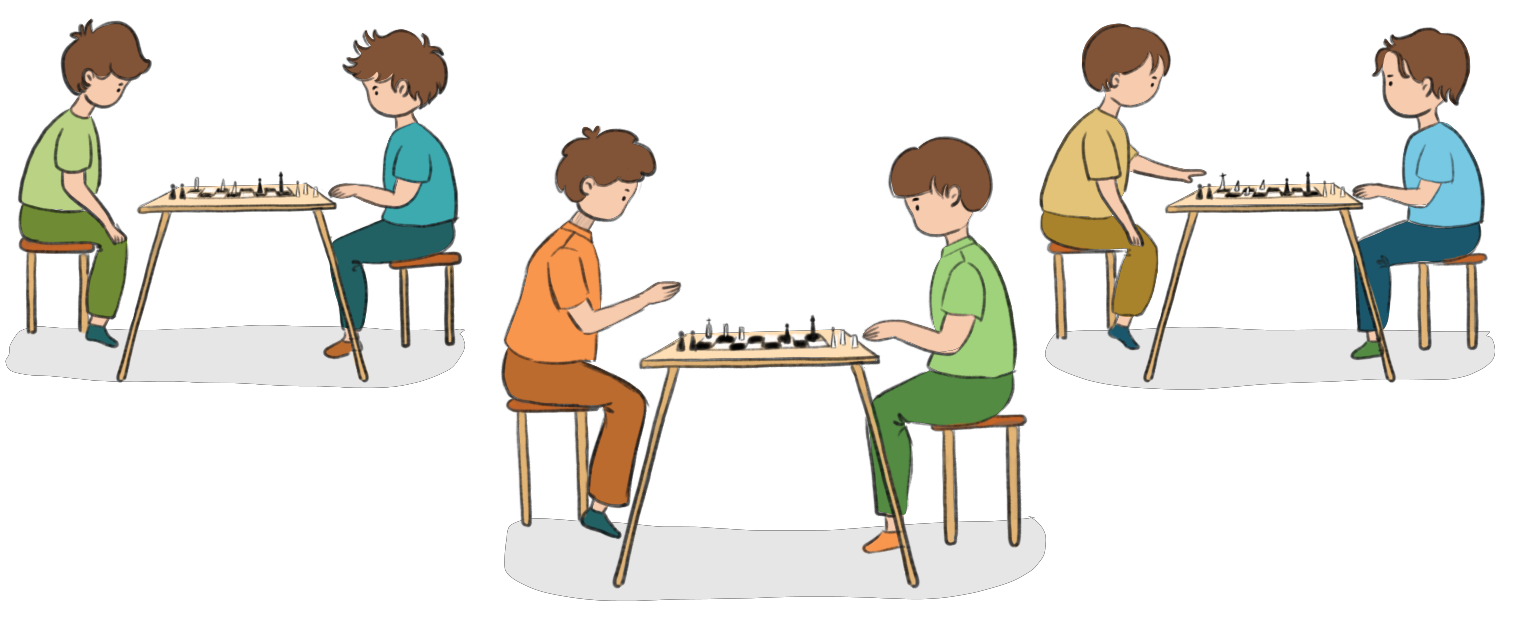
\includegraphics[width=1\linewidth]{Hinh1}
		\vspace*{-15pt}
	\end{figure}
	so với  tổng số hạt dẻ ở hai chiếc rương còn lại. Chiếc rương thứ hai có ít hơn $10$ hạt dẻ so với tổng số hạt dẻ ở chiếc rương thứ nhất và thứ ba. Hỏi trong chiếc rương thứ ba có bao nhiêu hạt dẻ?
	\vskip 0.1cm
	\textit{Lời giải.} 	Nếu ta lấy tổng số hạt dẻ ở rương thứ nhất và rương thứ hai, thì nhận được một số hạt dẻ nhỏ hơn tổng hạt dẻ ở rương thứ nhất, số hạt dẻ ở rương thứ hai và hai lần số hạt dẻ ở rương thứ ba là $6+10=16$ (hạt).
	\vskip 0.1cm
	Suy ra ở rương thứ ba có $16:2= 8$ (hạt dẻ).
	\vskip 0.1cm
	$\pmb{2.}$ Bạn Vân viết $150$ chữ số xung quanh một vòng tròn. Nếu đọc $150$ chữ số này theo chiều kim đồng hồ bắt đầu từ một chỗ nào đó bất kì, thì Vân thấy số nhận được chia hết cho $27$. Em hãy chứng minh rằng, nếu Vân bắt đầu từ bất kỳ một chỗ khác và đọc ngược chiều kim đồng hồ toàn bộ $150$ chữ số đã viết, thì bạn cũng nhận được một số chia hết cho $27$.
	\vskip 0.1cm
	\textit{Lời giải.} Khi xuất phát từ $1$ chữ số trên vòng tròn và đọc theo chiều kim đồng hồ, và khi xuất phát từ chữ số cuối cùng rồi đọc ngược chều kim đồng hồ ta thu được hai số có dạng $a\cdot10^k+b$  và $b\cdot 10^{150-k}+a$  với $k$ là số tự nhiên nào đó không vượt quá $150$. Nhân số thứ hai với $10^k$ (nguyên tố cùng nhau với $27$) rồi trừ đi số thứ nhất, ta nhận được số $b\cdot(10^{150}-1)$.
	\vskip 0.1cm 
	Do $(10^{150}-1) \,\vdots\, 10^3-1=999=37\times27$, số $b\cdot(10^{150}-1)$ chia hết cho $27$.
	\begin{figure}[H]
		\centering
		\vspace*{-5pt}
		\captionsetup{labelformat= empty, justification=centering}
		
\includegraphics[width=0.85\linewidth]{Hinh2}
		\vspace*{-5pt}
	\end{figure}
	Vậy nếu số thứ nhất chia hết cho $27$ thì số thứ hai cũng chia hết cho $27$.
	\vskip 0.1cm
	$\pmb{3.}$ Có ba tên cướp ăn trộm được $10$ viên kim cương trong một két sắt với tổng giá trị là $4 000 000$ dollar. Chúng dự định sẽ phân chia những viên kim cương này cho nhau để mỗi tên có được ít nhất $1 000 000$ dollar. Khi bị cảnh sát truy đuổi, một viên kim cương trị giá $600 000$ dollar bị rơi mất, và vì thế chúng không thể chia được những viên kim cương như dự định ban đầu. Hỏi ba tên cướp này có bị nhầm lẫn ở đâu không, hay là trước khi bị rơi viên kim cương, việc chia đồ ăn trộm của chúng đã không thể thực hiện được theo như dự định?
	\vskip 0.1cm
	\textit{Lời giải.} Nhận xét rằng nếu sau khi bị rơi mất $1$ viên kim cương, $9$ viên còn lại chia được như ý định ban đầu của bọn cướp thì với $10$ viên ban đầu cũng sẽ chia được như vậy. Giả sử $9$ viên còn lại có  $8$ viên có giá trị: $300.000$ và một viên $1.000.000$ thì việc chia chúng sẽ thực hiện được.
	\begin{figure}[H]
		\centering
		\vspace*{-5pt}
		\captionsetup{labelformat= empty, justification=centering}
		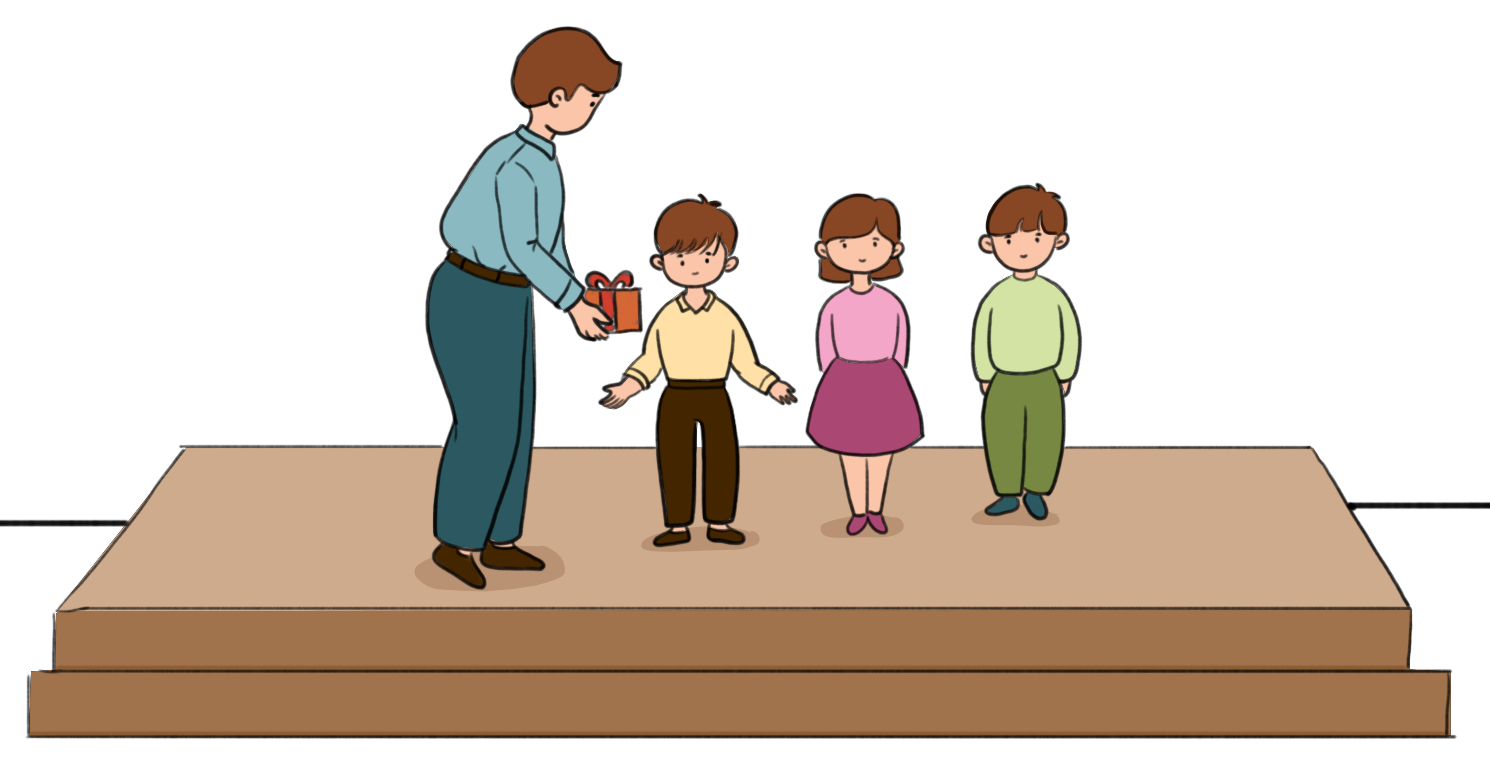
\includegraphics[width=1\linewidth]{Hinh3}
		\vspace*{-20pt}
	\end{figure}
	Ta cần xem xét xem liệu có trường hợp nào về giá trị của $10$ viên kim cương mà ban đầu thì chia được nhưng sau khi  rơi một viên như giả thiết và còn lại $9$ viên với tổng giá trị $3.400.000$ việc chia không còn thực hiện được hay không.
	Ta thấy điều này có thể xảy ra khi có những viên kim cương giá trị lớn trong khi những miếng có giá trị nhỏ dù gộp lại cũng không đủ $1.000.000$ đô la. Nói cách khác là khi giá trị của chúng rất chênh lệch. Giả sử  $10$ viên kim cương có  giá trị như sau:
	$1.400.000$;   $1.300.000$,  $600.000$;  và $7$ miếng còn lại có giá trị $100.000$.
	\vskip 0.1cm 
	Khi còn nguyên $10$ viên kim cương, ta có thể chia thành $3$ phần: $1.400.000$;   $1.300.000$, $1.300.000$.
	\vskip 0.1cm
	Khi mất viên thứ $3$ trị giá $600.000$ dollar, các tên cướp quả thật không thể chia số của cải ăn trộm theo như dự định ban đầu, và chúng đã không nhầm lẫn chút nào.
	\vskip 0.1cm
	$\pmb{4.}$ 	Bác Tâm mua một bao tải gạo nặng $9$ kg. Bác muốn chia ra thành hai túi nhỏ hơn, một túi nặng $2$ kg, còn túi kia nặng $7$ kg. Bác chỉ có một bàn cân đĩa thăng bằng với hai quả cân, một quả nặng $50$ g, còn quả kia nặng $200$ g. Em hãy giúp bác Tâm thực hiện phép san gạo ra hai túi nhỏ như trên chỉ tối đa sau ba lần cân.
	\vskip 0.1cm
	\textit{Lời giải.} Ta sẽ chỉ ra chỉ cần duy nhất $1$ quả cân nặng $200$ gr thì sau ba lần cân sẽ thực hiện được nhiệm vụ. Lần cân thứ nhất, ta đặt lên trên một đĩa cân quả cân trọng lượng $200$ gr, và đổ toàn bộ số gạo lên hai đĩa cân, sao cho hai bên thăng bằng. Khi đó một bên đĩa cân sẽ có $4$ kg $400$ g, còn bên kia có $4$ kg $600$~g.
	\begin{figure}[H]
		\centering
		\vspace*{-5pt}
		\captionsetup{labelformat= empty, justification=centering}
		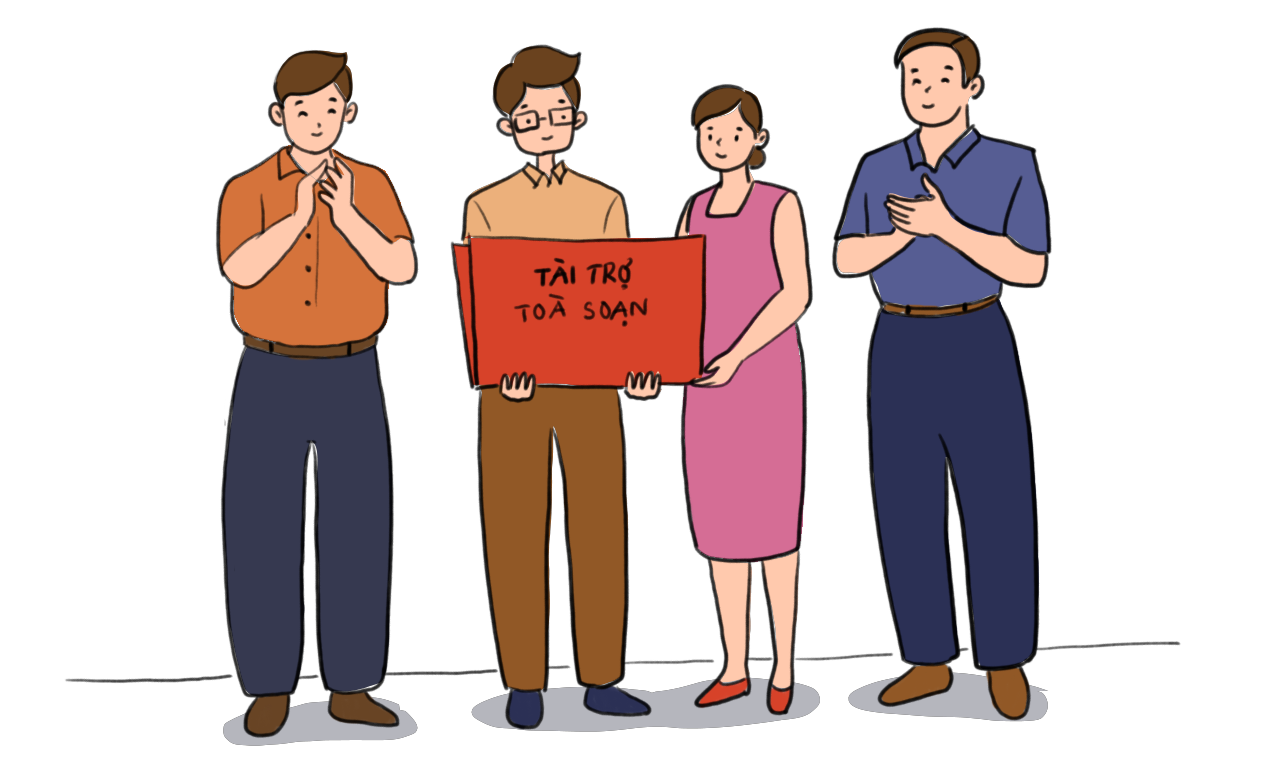
\includegraphics[width=1\linewidth]{Hinh4}
		\vspace*{-15pt}
	\end{figure}
	Lần cân thứ hai, làm tương tự, ta sẽ  đổ $4$ kg $600$ gr sang hai bên đĩa cân, để nhận được một bên có $2$ kg $400$ g và bên kia có $2$ kg $200$ g. Lần cân thứ ba, ta dùng quả cân trọng lượng $200$ g để lấy bớt được $200$ g từ đống gạo $2$ kg $200$ g để được $2$ kg gạo. Số gạo còn lại nặng $7$ kg.
	\vskip 0.1cm
	$\pmb{5.}$ 	Có $6$ đồng xu hình thức bên ngoài giống hệt nhau. Bốn đồng xu trong số đó là thật, mỗi đồng có khối lượng đúng $4$ g, còn hai đồng xu là giả có tổng khối lượng là $8$ g nhưng có một đồng nặng hơn một chút, còn một đồng nhẹ hơn một chút. Hỏi có thể sử dụng một bàn cân thăng bằng (không có quả cân) để sau tối đa bốn lần cân phát hiện được hai đồng xu giả được hay không?
	\begin{figure}[H]
		\centering
		\vspace*{-5pt}
		\captionsetup{labelformat= empty, justification=centering}
		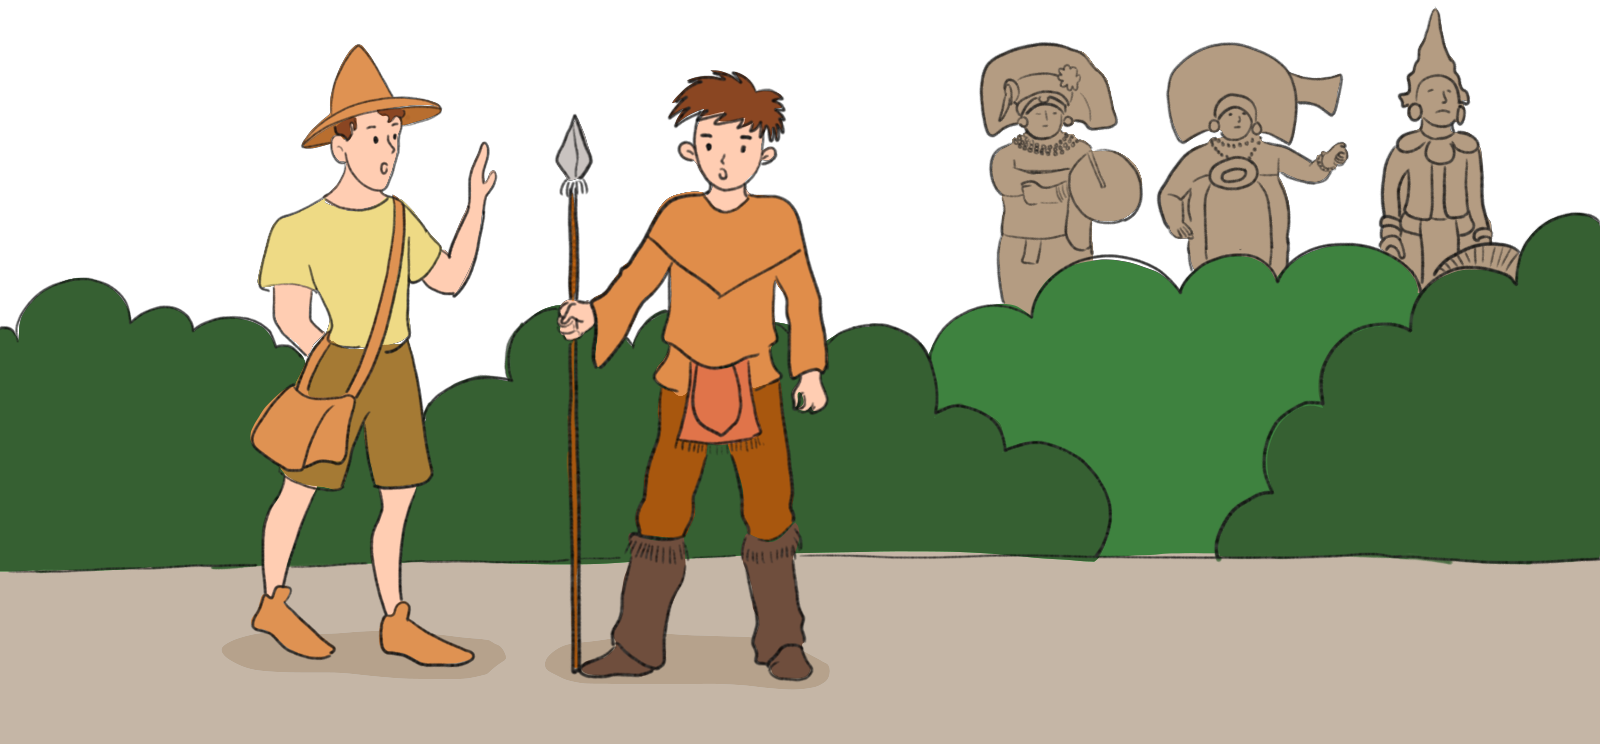
\includegraphics[width=1\linewidth]{Hinh5}
		\vspace*{-20pt}
	\end{figure}
	\textit{Lời giải.} Có thể. 
	\vskip 0.1cm
	Lần cân đầu tiên, ta đặt lên mỗi đĩa cân $3$ đồng xu. Khi đó có hai khả năng $A$ và $B$ sau.
	\vskip 0.1cm
	$A.$ Nếu hai đĩa cân thăng bằng, suy ra một đĩa cân có $3$ đồng xu thật có trọng lượng như nhau, và đĩa kia có $2$ đồng xu giả và $1$ đồng xu thật (gọi là $a,b$ và $c$) có trọng lượng khác nhau đôi một. 
	\vskip 0.1cm
	-- Tiếp theo ở lần cân thứ hai, ta lấy hai đồng xu ở một đĩa bất kỳ trong lần cân trước và đặt lên hai đĩa cân. 
	\vskip 0.1cm
	$+$ Nếu hai đĩa thăng bằng, thì hai đồng này là hai đồng xu thật. 
	\vskip 0.1cm
	$+$ Nếu hai đĩa không thăng bằng, thì hai đồng xu này đã được lấy ra từ $a, b, c$. Và như vậy, $3$ đồng xu của đĩa còn lại là xu thật.
	\vskip 0.1cm 
	Trong cả hai trường hợp ta đều xác định được đĩa có $3$ đồng xu thật. Bằng hai lần cân tiếp theo, với đồng xu thật làm tiêu chuẩn, ta dễ dàng tìm ra ngay đồng xu thật, và hai đồng xu giả trong số $a,b,c$.
	\vskip 0.1cm
	$B.$ Nếu hai đĩa không thăng bằng, suy ra  đĩa nhẹ  hơn  (gọi là đĩa $1$) chứa đồng xu giả nhẹ hơn $4$ g, còn đĩa bên kia (gọi là đĩa $2$) chứa đồng xu giả nặng hơn $4$ g.
	\vskip 0.1cm
	-- Ở lần cân thứ hai, nhặt hai đồng tuỳ ý ở đĩa $1$ và lại đặt lên cân. Nếu hai đồng này thăng bằng, thì đồng còn lại là giả. Còn nếu không thăng bằng, suy ra bên đĩa nào nhẹ hơn sẽ có đồng giả.
	\vskip 0.1cm
	-- Tương tự ở lần cân thứ ba, ta nhặt hai đồng tuỳ ý ở đĩa $B$ để phát hiện ra đồng giả nặng hơn trong số ba  xu ở đĩa $B$.
	\vskip 0.1cm
	Vậy ta có thể dùng tối đa $4$ lần cân để tìm hai đồng xu giả.
	\vskip 0.1cm
	$\pmb{6.}$ 	Trong một giải vô địch đá bóng của trường, đội dành huy chương vàng có được tổng số điểm là $7$, đội dành huy chương bạc có tổng số điểm là $5$, còn đội dành huy chương đồng có tổng số điểm là $3$. Biết rằng trong giải đấu này các đội thi đấu theo hình thức vòng tròn $1$ lượt, mỗi đội thi đấu với một đội khác đúng một trận, và trong mỗi trận mỗi đội sẽ nhận được $2$ điểm nếu thắng, $1$ điểm nếu hoà, $0$ điểm nếu thua. Nếu hai đội có cùng tổng số điểm thì vị trí thứ tự sẽ được xác định bằng hiệu số bàn thắng và bàn thua. Hỏi 
	\vskip 0.1cm
	$a)$ Đội đứng ở vị trí thấp nhất có được tổng số điểm là bao nhiêu?
	\vskip 0.1cm
	$b)$	Có bao nhiêu đội tham gia giải vô địch.
	\begin{figure}[H]
		\centering
		\vspace*{-10pt}
		\captionsetup{labelformat= empty, justification=centering}
		\includegraphics[width=1\linewidth]{Hinh6}
		\vspace*{-10pt}
	\end{figure}
	\textit{Lời giải.} Gọi số đội tham gia giải là $n$, khi đó tổng số điểm của tất cả $n$ đội trong giải vô địch bằng $n(n-1)$. Suy ra đội có nhiều điểm nhất phải dành được ít nhất $(n-1)$ điểm (là điểm trung bình của $n$ đội). 
	\vskip 0.1cm
	Tuy nhiên, theo đề bài, đội thứ nhất dành hơn điểm so với đội thứ hai, vì vậy đội đứng thứ nhất phải dành được ít nhất là $n$ điểm (nếu không đội đứng thứ hai cũng sẽ dành $(n-1)$ điểm).
	\vskip 0.1cm
	Do đội thứ nhất có tổng số điểm là $7$ nên $n\le7$. Ta lại có tổng số điểm của ba đội đứng đầu không vượt quá $n(n-1)$, suy ra $15\le n(n-1)$, từ đó ta có $n\ge5$.
	\vskip 0.1cm
	$\bullet$ Nếu $n=7$, suy ra tổng số điểm của $6$ đội còn lại là $7\times 6-7=35$. Do đó đội đứng thứ hai phải có ít nhất $[\dfrac{35}{6}]+1=6$ (điểm): mâu thuẫn.
	\vskip 0.1cm
	$\bullet$ Nếu $n=6$, tương tự, tổng số điểm của $3$ đội đứng cuối là $6\times 5-7-5-3=15$. Do đó sẽ có một đội trong số ba đội đứng cuối dành được ít nhất $5$ điểm. Mâu thuẫn, do đội đứng thứ ba chỉ dành được $3$ điểm.
	\vskip 0.1cm
	$\bullet$ Kết hợp lại, ta phải có $n=5$, tức là số đội tham gia giải là $5$ đội.
	\vskip 0.1cm
	Khi đó, tổng số điểm của hai đội đứng cuối là $5\times 4-7-5-3=5$ (điểm).
	\vskip 0.1cm
	Vì số điểm của mỗi đội trong số  hai đội đứng cuối không vượt quá $3$ điểm (đội đứng thứ ba được $3$ điểm), suy ra đội đứng ở vị trí thứ năm cuối cùng được $2$ điểm, và đội đứng thứ tư cũng được $3$ điểm (nhưng không được trao giải do thua kém hiệu số bàn thắng và bàn thua so với đội thứ ba). 
\end{multicols}
\newpage
\begingroup
\thispagestyle{toancuabinone}
\blfootnote{$^1$\color{toancuabi}Ottawa, Canada.}
\AddToShipoutPicture*{\put(60,733){\includegraphics[width=17.2cm]{../mathc.pdf}}}
%\AddToShipoutPicture*{\put(-2,733){\includegraphics[width=17.2cm]{../mathl.pdf}}} 
\AddToShipoutPicture*{\put(120,645){\includegraphics[scale=1]{../tieudec.pdf}}} 
\centering
\endgroup
\vspace*{60pt}

\begin{multicols}{2}
	In this article, we will discuss properties of perfect squares through a number of interesting examples.
	\vskip 0.2cm
	\PIbox{\textbf{\color{toancuabi}\color{toancuabi}Example $\pmb1$.}
		\textit{Cancelling the exponents} yields
		\begin{align*}
			\frac{37^3+13^3}{37^3+24^3} = \frac{37+13}{37+24} = \frac{50}{61}.
		\end{align*}
		which is correct.
		\vskip 0.1cm	
		Find the necessary and sufficient conditions for the positive integer triple $(A,B,C)$ to satisfy
		\begin{align*}
			\frac{A^3+B^3}{A^3+C^3} = \frac{A+B}{A+C}.
	\end{align*}}
	\vskip 0.1cm
	\textit{Solution.}
	For $A, B,$ and $C$ positive real numbers,
	\begin{align*}
		&\frac{A^3+B^3}{A^3+C^3} = \frac{A+B}{A+C} \\
		\Leftrightarrow\, &\frac{A^3+B^3}{A+B} = \frac{A^3+C^3}{A+C}\\
		\Leftrightarrow\, &A^2 - AB + B^2 = A^2 - AC + C^2\\
		\Leftrightarrow\, &(B-C)(A-B-C) = 0 \\
		\Leftrightarrow\, &{B=C} \text{\ or\ } {A = B+C.}
	\end{align*}
	\PIbox{
		\textbf{\color{toancuabi}\color{toancuabi}Example $\pmb2$.}
		For which natural number $n$ is $2^8 + 2^{11} + 2^n$ a perfect square?}
	\vskip 0.1cm
	\textit{Solution.}
	Let $m$ be an integer such that \linebreak $m^2 = 2^8 + 2^{11} + 2^n.$ Note that:
	\begin{align*}
		2^8 + 2^{11} = 2^8(1+2^3) = 2^8 \cdot 3^2 = 48^2.
	\end{align*}
	Thus,
	\begin{align*}
		2^n = m^2 - 48^2 = (m-48)(m+48).
	\end{align*}
	Therefore there exists positive integers $k, \ell,$ such that
	\begin{align*}
		&\left.
		\begin{aligned}
			m-48 &= 2^k \quad (1)\\
			m+48 &= 2^{\ell} \quad (2)\\
			k + \ell &= n
		\end{aligned}
		\right\}
		(2) - (1) \\
		\Rightarrow \,&96 = 2^5 \cdot 3 = 2^k(2^{\ell-k}-1)\\
		\Rightarrow \,&k = 5, \ell = 7 \Rightarrow {n = 12.}
	\end{align*}
	\PIbox{\textbf{\color{toancuabi}\color{toancuabi}Example $\pmb3$.}
		Prove that for $n$ positive integer the following number is a perfect square:
		\begin{align*}
			m = \underbrace{99 \ldots 9}_{n}\underbrace{00 \ldots 0}_{n}25.
	\end{align*}}
	\textit{Solution.}
	Note that $\underbrace{99 \ldots 9}_{n} = 10^n-1,$ thus:
	\begin{align*}
		m &= \underbrace{99 \ldots 9}_{n} 10^{n+2} + 25 \\
		&= 10^{2n+2} - 10^{n+2} + 25 = {(10^{n+1} - 5)^2.}
	\end{align*}
	\PIbox{\textbf{\color{toancuabi}\color{toancuabi}Example $\pmb4$.}
		Find all prime $p$ such that $2p^4-p^2 + 16$ is a perfect square.}
	\vskip 0.1cm
	\textit{Solution.}
	Note that a perfect square has a remainder $0$ or $1$ when divided by $3$.
	Thus 
	\begin{align*}
		&2p^4 \equiv 2p^2 \Mod{3} \\
		\Rightarrow \,&2p^4-p^2 + 16 \equiv p^2 + 1 \Mod{3}.
	\end{align*}	
	Since $2p^4-p^2 + 16$ is a perfect square, so $p^2 + 1 \equiv 0 \text{\ or\ } 1 \Mod{3} \Rightarrow {p = 3.}$
	In this case $2p^4-p^2 + 16 = 169 = 13^2.$
	\vskip 0.1cm
	\PIbox{\textbf{\color{toancuabi}\color{toancuabi}Example $\pmb5$.}
		Prove that the sum of the squares of $1984$ consecutive positive integers cannot be the square of an integer.}
	\vskip 0.2cm
	\textit{Solution.}
	Let $n \ge 0$ be an integer. Let $S(n, k) = (n+1)^2 + (n+2)^2 + \cdot + (n+k)^2,$ where $k$ is a positive integer, then:
	\begin{align*}
		&S(n, k) \\
		= \,&kn^2 + 2n(1+2+\cdot +k)\\
		&+(1^2+2^2+\cdots+k^2)\\
		= \,&kn^2 + nk(k+1) + \frac{k(k+1)(2k+1)}{6}.
	\end{align*}		
	With $k=1984,$ 
	\begin{align*}
		&S(n, 1984) \\
		= \,&992 (2n^2+(2\cdot 1985)n+ 1985\cdot 1323).
	\end{align*}
	Since the second term of $S(n, 1984)$ is an odd number and $992 = 2^5 \cdot 31,$ $S(n, 1984)$ is divisible by $2^5,$ 
	but not by $2^6.$ Hence, it is not a perfect square.
\end{multicols}